% Suppress PDF creation date and local timezone metadata
\pdfinfoomitdate=1
\pdftrailerid{}
\pdfsuppressptexinfo=-1
\documentclass[11pt,a4paper]{article}

\usepackage[T1]{fontenc}
\usepackage{lmodern}
\usepackage[a4paper, margin=1in, bottom=1.15in, footskip=0.45in]{geometry}
\usepackage{amsmath,amssymb,amsfonts}
\usepackage{graphicx}
\usepackage{booktabs}
\usepackage{xcolor}
\usepackage{array}
\usepackage{url}
\def\UrlBreaks{\do\/\do-\do\_\do\.\do\a\do\b\do\c\do\d\do\e\do\f\do\g\do\h\do\i\do\j\do\k\do\l\do\m\do\n\do\o\do\p\do\q\do\r\do\s\do\t\do\u\do\v\do\w\do\x\do\y\do\z}
\usepackage[numbers,sort&compress]{natbib}
\makeatletter
\def\fnum@figure{\textbf{Fig.~\thefigure}}
\def\fnum@table{\textbf{Table~\thetable.}}
\long\def\@makecaption#1#2{%
  \vskip\abovecaptionskip
  \sbox\@tempboxa{#1 #2}%
  \ifdim \wd\@tempboxa >\hsize
    #1 #2\par
  \else
    \global \@minipagefalse
    \hb@xt@\hsize{\hfil\box\@tempboxa\hfil}%
  \fi
  \vskip\belowcaptionskip}
\makeatother
\usepackage[colorlinks=true, linkcolor=blue, citecolor=blue, urlcolor=blue]{hyperref}

\pagestyle{plain}
\newtheorem{remark}{Remark}

\begin{document}

\title{\LARGE \textbf{Disentangling Evaluation Distortions in 2D-to-3D Brain Tumor MRI Segmentation: A Patient-Grouped Leakage, Calibration, and Volumetric Post-Processing Audit on TCGA-LGG}}

\author{Shayan Ganji Nataj$^{1}$ \and Keivan Borna$^{1,*}$}

\date{\small $^{1}$Department of Computer Science, Faculty of Mathematics and Computer Science, Kharazmi University, Tehran, Iran\\[0.3em]
$^{*}$Corresponding Author: \texttt{borna@khu.ac.ir}}

\maketitle

\begin{abstract}
Lower-grade glioma benchmarks report high Dice, but clinical translation is hindered by evaluation flaws. Auditing TCGA-LGG (110 patients, 3,929 slices) disentangles leakage, dilution, calibration, and post-processing across 5 folds. Patient-grouped Attention Res-UNet achieves 73.96\% positive-slice ($\text{Dice}_{\text{pos}}$) and 82.02\% all-slice Dice. Random-slice splitting inflates positive-slice Dice by $+8.79\,\text{pp}$ [95\% CI: $+6.16, +11.99\,\text{pp}$] (82.74\%; patient median inflation $4.41\,\text{pp}$, IQR: $1.08$--$10.74\,\text{pp}$) and all-slice Dice by $+6.20\,\text{pp}$ [95\% CI: $+4.26, +8.31\,\text{pp}$] ($88.22\%$). A copy oracle reaches 86.18\% all-slice Dice via empty copying ($\text{FPR}_{\text{empty}} = 0.63\%$), while per-patient inflation is decoupled from mask continuity ($r = -0.068$) and persists across non-adjacent slices (primarily at a 2-slice gap, $\Delta z \ge 2$: $+5.54\,\text{pp}$). A non-lesional probe predicts patient identity with 79.64\% accuracy (82.32\% at $\Delta z = 1$, 59.44\% at $\Delta z \ge 2$), indicating patient cues, though background similarity does not predict inflation. Scoring empty slices as true negatives shifts all-slice over positive-slice Dice by $+8.06$ to $+15.64\,\text{pp}$ across post-processing rules (Largest-CC: 89.64\% vs.\ 74.00\%), yielding no detectable rank agreement ($\tau = -0.067$) and reversing top ranks below $\pi^* = 86.53\%$. Weighted active-bin calibration error fell from 36.14\% to 29.57\% under temperature scaling and to 8.46\% under affine Platt scaling with neutral overlap. Training-patient conformal calibration reduced test coverage to 76.96\% (median 85.87\%), whereas out-of-patient calibration reached 85.74\% (median 94.29\%, 87.69\% under CRC, 90.08\% at $n_{\text{cal}} = 30$). Axial z-rescue (CAL-3DH) restored polar margins across 17 volumes (+0.28 pp, $p_{\text{Holm}} = 0.0011$) without surface penalty ($\text{ASD} = 1.96$ vs.\ 1.95).
\end{abstract}

\vspace{0.8em}
\noindent\textbf{Keywords:} Brain tumor MRI segmentation, Data leakage, Evaluation distortions, Probability calibration, Conformal prediction, 3D volumetric post-processing.

\vspace{1.5em}

\section{Introduction}
\label{sec:intro}

Lower-grade gliomas (LGG), encompassing World Health Organization (WHO) grade II and grade III astrocytomas and oligodendrogliomas, represent diffusely infiltrative primary brain neoplasms characterized by substantial histological and genetic heterogeneity~\cite{louis20212021,ceccarelli2016molecular}. Accurate volumetric delineation on magnetic resonance imaging (MRI) is essential for image-guided maximal surgical resection, conformal radiation planning, and monitoring therapeutic response~\cite{buda2019association}. Over the past decade, deep learning architectures---most notably 2D U-Net variants~\cite{ronneberger2015u,zhou2018unetplusplus,oktay2018attention}---have emerged as the prevailing standard for automated lesion delineation. 

Despite reported segmentation accuracies exceeding an $80\%$ Dice similarity coefficient across benchmark datasets, our audit reveals a multi-layer evaluation distortion and leakage budget that undermines empirical validity in the medical computing literature across four distinct levels: (i)~\textbf{Inter-Slice Partition Leakage and Feature Memorization:} Decomposing volumetric MRI scans into independent 2D axial slices and randomly partitioning them across splits allows contiguous slices from the same patient to appear across training and test sets. Deep networks can exploit within-patient inter-slice correlation and contiguous anatomical continuity, artificially inflating positive-slice Dice by $+8.79\text{ pp}$ ($73.96\%$ to $82.74\%$, $+11.88\%$ relative distortion, 95\% CI: $[+6.16, +11.99]\text{ pp}$) and all-slice Dice by $+6.20\text{ pp}$ ($95\%$ CI: $[+4.26, +8.31]\text{ pp}$); as our zero-parameter nearest-slice label-copy oracle demonstrates, an all-slice Dice of $86.18\%$ is attainable purely from contiguous label adjacency without any deep neural network (coming within $2.04\text{ pp}$ of the deep network, $88.22\%$, because empty-slice status is near-perfectly copied with $\text{FPR}_{\text{empty}} = 0.63\%$ vs.\ $8.84\%$, despite lagging by $21.13\text{ pp}$ on positive tumor slices: $61.61\%$ vs.\ $82.74\%$); furthermore, a non-lesional brain appearance probe retrieves exact patient identity with $79.64\%$ accuracy ($82.32\%$ at $\Delta z = 1$, $59.44\%$ at $\Delta z \ge 2$) across random-split partitions (vs.\ $0.91\%$ random chance), demonstrating that axial slices carry strong patient-specific textural signatures across the volume; (ii)~\textbf{Empty-Slice Metric Dilution and Rank Inversion ($\pi^*$):} Because $65.05\%$ of slices in the TCGA-LGG cohort are tumor-free ($2,556 / 3,929$), evaluating all slices with $\text{Dice} = 1.0$ when both prediction and ground truth are empty inflates all-slice mean Dice ($\text{Dice}_{\text{all}}$) by $+8.06\text{ pp}$ to $+15.64\text{ pp}$ over positive-slice Dice ($\text{Dice}_{\text{pos}}$), which analytically reverses pairwise rankings below $\pi^* = 86.53\%$ and empirically decorrelates cohort rankings; (iii)~\textbf{Principled Nested Threshold Selection vs.\ Post-Hoc Sweeping:} Moving from the arbitrary default threshold $\tau=0.50$ to the inner-fold optimal threshold $\tau_{xy}^* = 0.74$ yields a modest $+0.64\text{ pp}$ gain on positive slices ($+2.43\text{ pp}$ on all slices), representing principled inner-fold tuning, whereas sweeping thresholds directly over pooled test sets introduces an optimism bias of $\Delta\text{Optimism} = +0.063\text{ pp}$; and (iv)~\textbf{Calibration Monotonicity Invariance and Conformal Safety Degradation:} While temperature scaling and affine Platt scaling effectively regularize active-bin calibration errors without altering spatial overlap (Remark~1), calibrating conformal thresholds on in-sample training-patient calibration sets causes substantial empirical patient-level coverage reduction (from nominal $90\%$ to $76.96\% \pm 22.46\%$, median $85.87\%$) when deployed on unseen patients, whereas honest patient-grouped calibration achieves $85.74\% \pm 21.34\%$ (median $94.29\%$). This demonstrates that calibrating conformal thresholds on training-patient slices (violating calibration-test subject independence) induces substantial under-coverage on unseen patients.

Beyond evaluation methodology, 2D networks face fundamental domain-specific limitations when applied to volumetric scans. Overlap-based loss formulations like Focal Tversky prioritize rare foreground voxels by heavily down-weighting easy background terms, causing output probabilities to become overconfident and miscalibrated. Furthermore, because $65.05\%$ of all axial slices in the TCGA-LGG cohort are healthy brain tissue containing zero neoplastic voxels, standard 2D networks lacking cross-slice volumetric context frequently trigger false-positive alarms on non-tumor slices while failing to detect small infiltrative margins at apical and basal tumor boundaries.

To address these questions, we conduct a controlled methodological audit on the complete TCGA-LGG cohort (110 patients, 3,929 slices)~\cite{buda2019association}, evaluating a modular post-processing case study (CAL-3DH) alongside simple 3D morphological baselines. The contributions of this study are fourfold:

\begin{enumerate}
    \item \textbf{Empirical Leakage Quantification, Appearance Probe, \& Mask Continuity Index (MCI):} We implement a matched 5-fold cross-validation audit comparing patient-grouped against random-slice partitioning under identical architecture controls, quantifying the $+8.79\text{ pp}$ ($95\%$ CI: $[+6.16, +11.99]\text{ pp}$) inflation on positive-slice Dice. We establish a zero-parameter copy oracle ($86.18\%$ all-slice Dice via empty-slice copying), formulate an Inter-Slice Mask Continuity Index ($\text{MCI} = 0.730 \pm 0.078$), establish that matched leakage inflation persists across non-adjacent slices (primarily at a 2-slice gap, $\Delta z \ge 2$: $+5.54\text{ pp}$), and design a non-lesional brain texture probe demonstrating $79.64\%$ patient identity retrieval ($82.32\%$ at $\Delta z = 1$, $59.44\%$ at $\Delta z \ge 2$ vs.\ $0.91\%$ chance), indicating high patient-identifying information in non-lesional slices, although neither mask continuity nor background similarity linearly predicts per-patient inflation magnitude.
    \item \textbf{Analytical Metric Dilution, Critical Rank Inversion ($\pi^* = 86.53\%$), \& Multifocal Lesion Preservation:} We derive the closed-form identity connecting all-slice Dice to empty-slice false positive rate and identify the critical prevalence threshold $\pi^* = 86.53\%$, analytically explaining why all-slice evaluation in whole-brain MRI ($\pi = 34.95\%$) decorrelates method rankings and reverses top ranks between global false-positive suppression (Largest-CC, which removes secondary foci) and boundary-recovery rules in multifocal tumors. A $2^3$ factorial attribution decomposes total inflation ($+18.14\text{ pp}$) into metric dilution ($45.7\%$), leakage ($40.8\%$), and post-processing/thresholding ($13.5\%$).
\item \textbf{Calibration Monotonicity Invariance (Remark 1) and Conformal Safety Degradation:} We establish that strictly monotonic probability calibration preserves validation-optimized spatial overlap (Remark~1). Furthermore, evaluating conformal threshold calibration demonstrates that tuning under in-sample training-patient calibration (where slices from training patients overlap into calibration) causes empirical patient-level test coverage on unseen clinical subjects to drop to $76.96\% \pm 22.46\%$ (median $85.87\%$), whereas honest out-of-patient calibration achieves $85.74\% \pm 21.34\%$ (SD across patients) (median $94.29\%$, with patient-level conformal risk control reaching $87.69\% \pm 19.18\%$, and $90.08\% \pm 1.86\%$ (SD across MC resamplings with $n_{\text{cal}} = 30$)).
    \item \textbf{Comparative 3D Post-Processing Audit (CAL-3DH) \& Multi-Site Radiogenomics:} We benchmark simple 3D heuristics against conditional axial z-rescue, revealing that while simple component filtering dominates global 3D surface metrics, axial z-rescue specifically restores truncated polar boundary margins across 17 volumes ($+0.28\text{ pp}$ positive-slice Dice, $p_{\text{Holm}} = 0.0011$) without altering 3D surface distances ($\text{ASD}: 1.96$ vs.\ $1.95\text{ voxels}$). Reconstructed volumes show good volumetric consistency ($\text{ICC}(2,1) = 0.8894$), while multi-institutional stratification across the five TCGA source sites quantifies cross-site performance variability and exploratory covariate-adjusted radiogenomic trends ($p = 0.056$).
\end{enumerate}

The combination of controlled leakage auditing, probability calibration, 3D volumetric post-processing, and multi-site radiogenomics provides a transparent, patient-disjoint benchmarking template for volumetric neuro-oncology.

\subsection{Related Work on Segmentation Calibration and Data Leakage}
\label{sec:related_work}
Automated glioma segmentation has advanced substantially through 2D and 3D deep convolutional networks, spanning classical U-Net architectures~\cite{ronneberger2015u,buda2019association}, attention gating~\cite{oktay2018attention}, and multi-scale nested feature decoders~\cite{zhou2018unetplusplus}. To counter acute foreground-background class imbalance in brain MRI, modern architectures predominantly employ overlap-based objective functions such as Tversky and Focal Tversky losses~\cite{salehi2017tversky,abraham2019novel}. While these formulations maximize spatial overlap, Guo et al.~\cite{guo2017calibration} demonstrated that modern neural networks frequently suffer from probability miscalibration, while Mehrtash et al.~\cite{mehrtash2020confidence}, Mukhoti et al.~\cite{mukhoti2020calibrating}, and Jungo and Reyes~\cite{jungo2019assessing} demonstrated that overlap-loss training produces overconfident predictions along ambiguous tissue interfaces that compromise clinical interpretability and distort post-processing threshold sweeps. Concurrently, data leakage arising from random slice-level partitioning in volumetric imaging has emerged as a pervasive threat to methodological validity in computational medicine~\cite{wen2020convolutional}. When contiguous 2D axial slices from the same subject are distributed across training and test splits, deep networks can exploit within-patient inter-slice correlation and anatomical continuity across contiguous slices, generating artificially inflated performance metrics that fail to reflect generalization to unseen clinical subjects~\cite{kapoor2023leakage,varoquaux2022machine,yagis2021effect}. By integrating rigorous patient-grouped partitioning with nested temperature scaling and conditional axial 3D spatial continuity, CAL-3DH systematically unites evaluation integrity with probabilistic reliability and volumetric coherence.

Recent auditing initiatives in brain tumor MRI have further exposed the pervasive confounding impact of benchmark contamination and unverified dataset provenance. Notably, Uddin and Ferdouse~\cite{uddin2026data} systematically demonstrated that image-level partitioning across public brain tumor classification benchmarks artificially inflates model accuracy to $97.10\%$ compared to $91.82\%$ under patient-level splitting ($p=0.017$, Welch's $t$-test) on the benchmark subset providing patient identifiers, with true-duplicate leakage contaminating evaluation splits across multiple widely used public repositories. In this study, we extend this rigorous auditing paradigm from 2D classification to 3D volumetric lower-grade glioma segmentation and probability calibration on clinical TCGA-LGG acquisitions.

\section{Materials and Methods}
\subsection{Cohort Characteristics and Clinical Variables}
Experiments were conducted using the standardized TCGA-LGG MRI collection introduced by Buda et al.~\cite{buda2019association}, curated by The Cancer Imaging Archive (TCIA)~\cite{clark2013cancer,pedano2016cancer} (persistent DOI: \url{https://doi.org/10.7937/K9/TCIA.2016.L4LTD3TK}), comprising 110 patients diagnosed with WHO grade II or III lower-grade gliomas. Each patient study consists of axial multi-sequence MRI slices (fluid-attenuated inversion recovery [FLAIR], T1-pre, and T1-post contrast) mapped into $256 \times 256$ matrices with matched manual FLAIR-abnormality reference segmentations verified by a board-eligible radiologist~\cite{buda2019association}. The full imaging volume encompasses 3,929 paired axial slices. Per SAGER reporting guidelines, the cohort includes 56 female patients ($50.9\%$) and 53 male patients ($48.2\%$), with sex recorded as unknown for one patient. Matched clinical and genomic records were extracted from the companion table \texttt{data.csv} distributed with the TCGA-LGG benchmark~\cite{buda2019association,pedano2016cancer}, originally curated from the TCGA pan-glioma genomic study~\cite{ceccarelli2016molecular} (Table~\ref{tab:clinical_cohort}). One subject has missing (NA) demographic and histological grade entries in \texttt{data.csv} (accounting for the single unknown sex and grade entries in Table~\ref{tab:clinical_cohort}) while retaining an assigned genomic cluster label, and is retained in all imaging analyses; the raw \textit{COCCluster} counts in \texttt{data.csv} ($56/24/30$, summing to $110$) differ by one subject from the printed summary in~\cite{buda2019association} ($55/25/30$) and are analyzed verbatim as distributed in the repository.

\begin{table}[tbp]
\centering
\caption{Clinical, histological, and genomic characteristics of the 110 patients in the TCGA-LGG cohort.}
\label{tab:clinical_cohort}
\setlength{\tabcolsep}{8pt}
\small
\begin{tabular*}{\textwidth}{@{\extracolsep{\fill}}llr}
\toprule
\textbf{Clinical Variable} & \textbf{Category / Unit} & \textbf{Value / Count} \\
\midrule
Total Patients ($N$) & Subjects & 110 \\
Total Axial Slices & Slices & 3,929 \\
Tumor-Bearing Slices & Slices ($y > 0$) & 1,373 (34.95\%) \\
Tumor-Free Slices & Slices ($y = 0$) & 2,556 (65.05\%) \\
\midrule
Patient Sex & Female ($n=56$) & 50.9\% \\
(SAGER Reporting) & Male ($n=53$) & 48.2\% \\
 & Unknown ($n=1$) & 0.9\% \\
Patient Age & Mean $\pm$ SD (years) & 47.1 $\pm$ 13.4 \\
& Range (Min -- Max) & 20.0 -- 75.0 \\
\midrule
WHO Histologic Grade & Grade II ($n=51$) & 46.4\% \\
& Grade III ($n=58$) & 52.7\% \\
& Unspecified ($n=1$) & 0.9\% \\
\midrule
Molecular Subtypes & COC 1 (IDHmut-noncodel) & 56 (50.9\%) \\
(\textit{COCCluster}) & COC 2 (IDH-wt like) & 24 (21.8\%) \\
& COC 3 (IDHmut-codel) & 30 (27.3\%) \\
\bottomrule
\end{tabular*}
\end{table}

\subsection{Quality-Aware Screening and Wavelet Denoising}
Prior to model training, raw axial slices were analyzed for pronounced imaging artifacts and skull-stripping failures using three complementary morphological descriptors. First, parenchymal texture insufficiency was quantified via Edge Density ($ED$), defined as the proportion of Canny edge pixels (thresholds 50 and 150) following morphological dilation with a $5 \times 5$ square structuring element, normalized by image area:
\begin{equation}
ED = \frac{|E_{\text{dilated}}|}{H \times W}
\end{equation}
where slices satisfying $ED < 0.003$ exhibit negligible brain tissue. Second, anatomical field-of-view truncation was evaluated through the Contour Ratio ($CR$), defined as the area of the largest closed external contour extracted from the dilated edge map divided by image area:
\begin{equation}
CR = \frac{\text{Area}(\mathcal{C}_{\text{largest}})}{H \times W}
\end{equation}
where $CR < 0.01$ flags severe field truncation. Third, decentering was assessed by the Centroid Distance ($d_c$), defined as the Euclidean distance from the external contour centroid $(c_x, c_y)$ to the geometric slice center normalized by the half-diagonal:
\begin{equation}
d_c = \frac{\sqrt{(c_x - W/2)^2 + (c_y - H/2)^2}}{\sqrt{(W/2)^2 + (H/2)^2}}
\end{equation}
where $d_c > 0.30$ captures severe peripheral displacement.

Slices satisfying the conjunction $(ED < 0.003) \land (CR < 0.01) \land (d_c > 0.30)$ were flagged as morphological artifacts. A rigorous cohort audit across all 3,929 slices identified 200 artifact slices ($5.09\%$, Table~\ref{tab:screening_audit}). Exactly 199 of these 200 slices ($99.50\%$) contained zero neoplastic tissue ($y = 0$). Only a single slice ($0.50\%$, Slice 23 of TCGA\_DU\_5855) contained a marginal peripheral tumor component truncated by skull-stripping boundary erosion. Crucially, while 200 slices ($5.09\%$) were flagged across the full 3,929-slice cohort, only the flagged slices falling within each fold's 75-patient training split ($\approx 136$ artifact slices per fold, leaving $\approx 2,535$ clean training slices per fold) were excluded during model weight optimization, while all internal validation (\texttt{inner\_val}, 13 patients) and untouched outer test evaluations (\texttt{outer\_test}, 22 patients) were conducted on the complete, unfiltered slices (with Table~\ref{tab:screening_audit} and Table~\ref{tab:baseline_performance} additionally displaying the 3,729-slice screened comparison). Retaining these 200 noisy slices in the untouched test evaluation confirmed an absolute $0.00\text{ pp}$ change in positive-slice Dice ($73.96\%$ in both full and screened cohorts), showing no observable change at two-decimal reporting precision. All 2D and 3D volumetric and surface distance metrics ($\text{HD}_{95}$, $\text{ASD}$, volumes) are evaluated on the standardized $128 \times 128$ in-plane grid in voxel units because the public Kaggle/TCIA TIFF distribution does not retain raw DICOM physical millimeter spacing metadata.

\begin{table}[tbp]
\centering
\caption{Screening audit of the 200 artifact slices excluded during training.}
\label{tab:screening_audit}
\setlength{\tabcolsep}{8pt}
\small
\begin{tabular*}{\textwidth}{@{\extracolsep{\fill}}lrr}
\toprule
\textbf{Screening Metric} & \textbf{Flagged Slices} & \textbf{Ratio (\%)} \\
\midrule
Total Slices Screened & 3,929 & 100.0\% \\
Total Artifact Slices Excluded & 200 & 5.09\% \\
\midrule
\hspace{1.2em}Empty Slices (Zero Tumor, $y=0$) & 199 / 200 & \textbf{99.50\%} \\
\hspace{1.2em}Marginal Slices (Atypical Clipping) & 1 / 200 & 0.50\% \\
\hspace{1.2em}Edge Density Violation ($ED < 0.003$) & 200 / 200 & 100.0\% \\
\hspace{1.2em}Contour Ratio Violation ($CR < 0.01$) & 200 / 200 & 100.0\% \\
\hspace{1.2em}Centroid Distance Violation ($d_c > 0.30$) & 200 / 200 & 100.0\% \\
\hspace{1.2em}Triple Conjunction Violation & 200 / 200 & \textbf{100.0\%} \\
\midrule
Positive-Slice Dice on Full Cohort (3,929) & \multicolumn{2}{c}{73.96\% [70.10 -- 77.15]} \\
Positive-Slice Dice on Screened (3,729) & \multicolumn{2}{c}{73.96\% [70.10 -- 77.13]} \\
\textbf{Absolute Impact on Positive Dice} & \multicolumn{2}{c}{\textbf{0.00\% (Identical)}} \\
\bottomrule
\end{tabular*}
\end{table}

To suppress high-frequency acquisition noise while retaining crisp anatomical borders, slices were processed using BayesShrink soft-thresholded discrete wavelet denoising~\cite{chang2000adaptive} conditioned on a localized slice quality metric $Q(I)$:
\begin{equation}
Q(I) = \frac{1}{2}\Big[\sigma\big(I - \mathcal{M}_{3\times 3}(I)\big) + \sigma\big(I - \mathcal{G}_{3\times 3}(I)\big)\Big]
\end{equation}
representing the average standard deviation of high-frequency residuals under $3 \times 3$ median ($\mathcal{M}_{3\times 3}$) and Gaussian ($\mathcal{G}_{3\times 3}$) spatial filters. The localized quality index $Q(I)$ was evaluated across all 3,929 cohort slices (routing 3,738 slices with $Q(I) < 4.0$ [$95.14\%$] to BayesShrink wavelet denoising [Symlet-4 wavelet, 2-level decomposition] and 191 slices with $Q(I) \ge 4.0$ [$4.86\%$] to high-contrast bypass avoiding unnecessary smoothing of delicate parenchymal boundaries; Figure~\ref{fig:preprocessing_audit}), while flagged training-split artifact slices ($\approx 136$ per fold) were excluded prior to network weight optimization. All quality screening thresholds ($\text{ED} < 0.003$, $\text{CR} < 0.01$, $d_c > 0.30$, and $Q < 4.0$) were pre-specified morphologically on domain considerations prior to model training without test set inspection. Slices were standardized to zero mean and unit variance and resized to $128 \times 128 \times 3$ to ensure computational tractability for exhaustive nested inner-fold grid searches, multi-stage 3D ablations, and $10,000$-iteration patient-clustered bootstrap evaluations across both split regimes.

\begin{figure}[tbp]
\centering
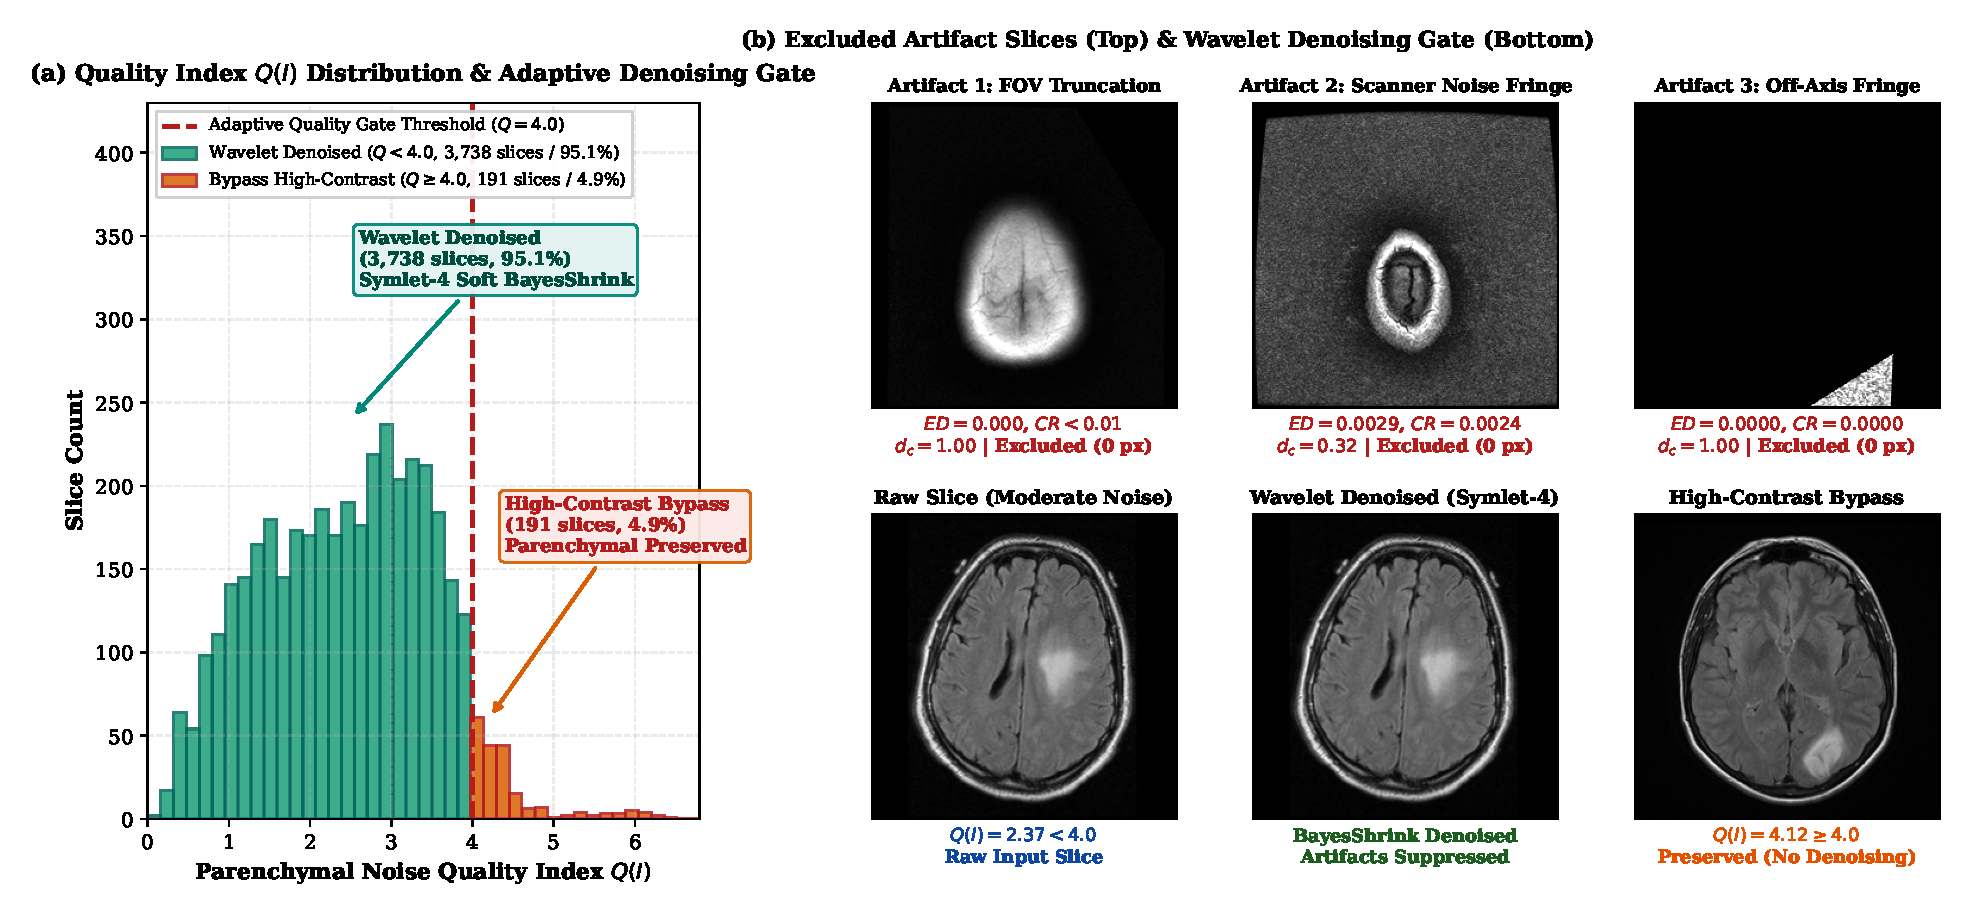
\includegraphics[width=\textwidth]{Fig1.pdf}
\caption{Quality-aware preprocessing and screening audit across the TCGA-LGG cohort (3,929 axial slices). (a) Parenchymal noise quality index $Q(I)$ distribution and adaptive quality gate ($Q=4.0$), routing 3,738 slices ($95.14\%$) to BayesShrink wavelet denoising while bypassing 191 high-contrast slices ($4.86\%$). (b) Representative real MRI slice examples: top row displays three of the 200 artifact slices excluded during training (illustrating field-of-view truncation, scanner noise fringe, and non-parenchymal tissue with exact $ED, CR, d_c$ metrics); bottom row compares raw, wavelet-denoised, and high-contrast bypass slices}
\label{fig:preprocessing_audit}
\end{figure}

\begin{figure}[tbp]
\centering
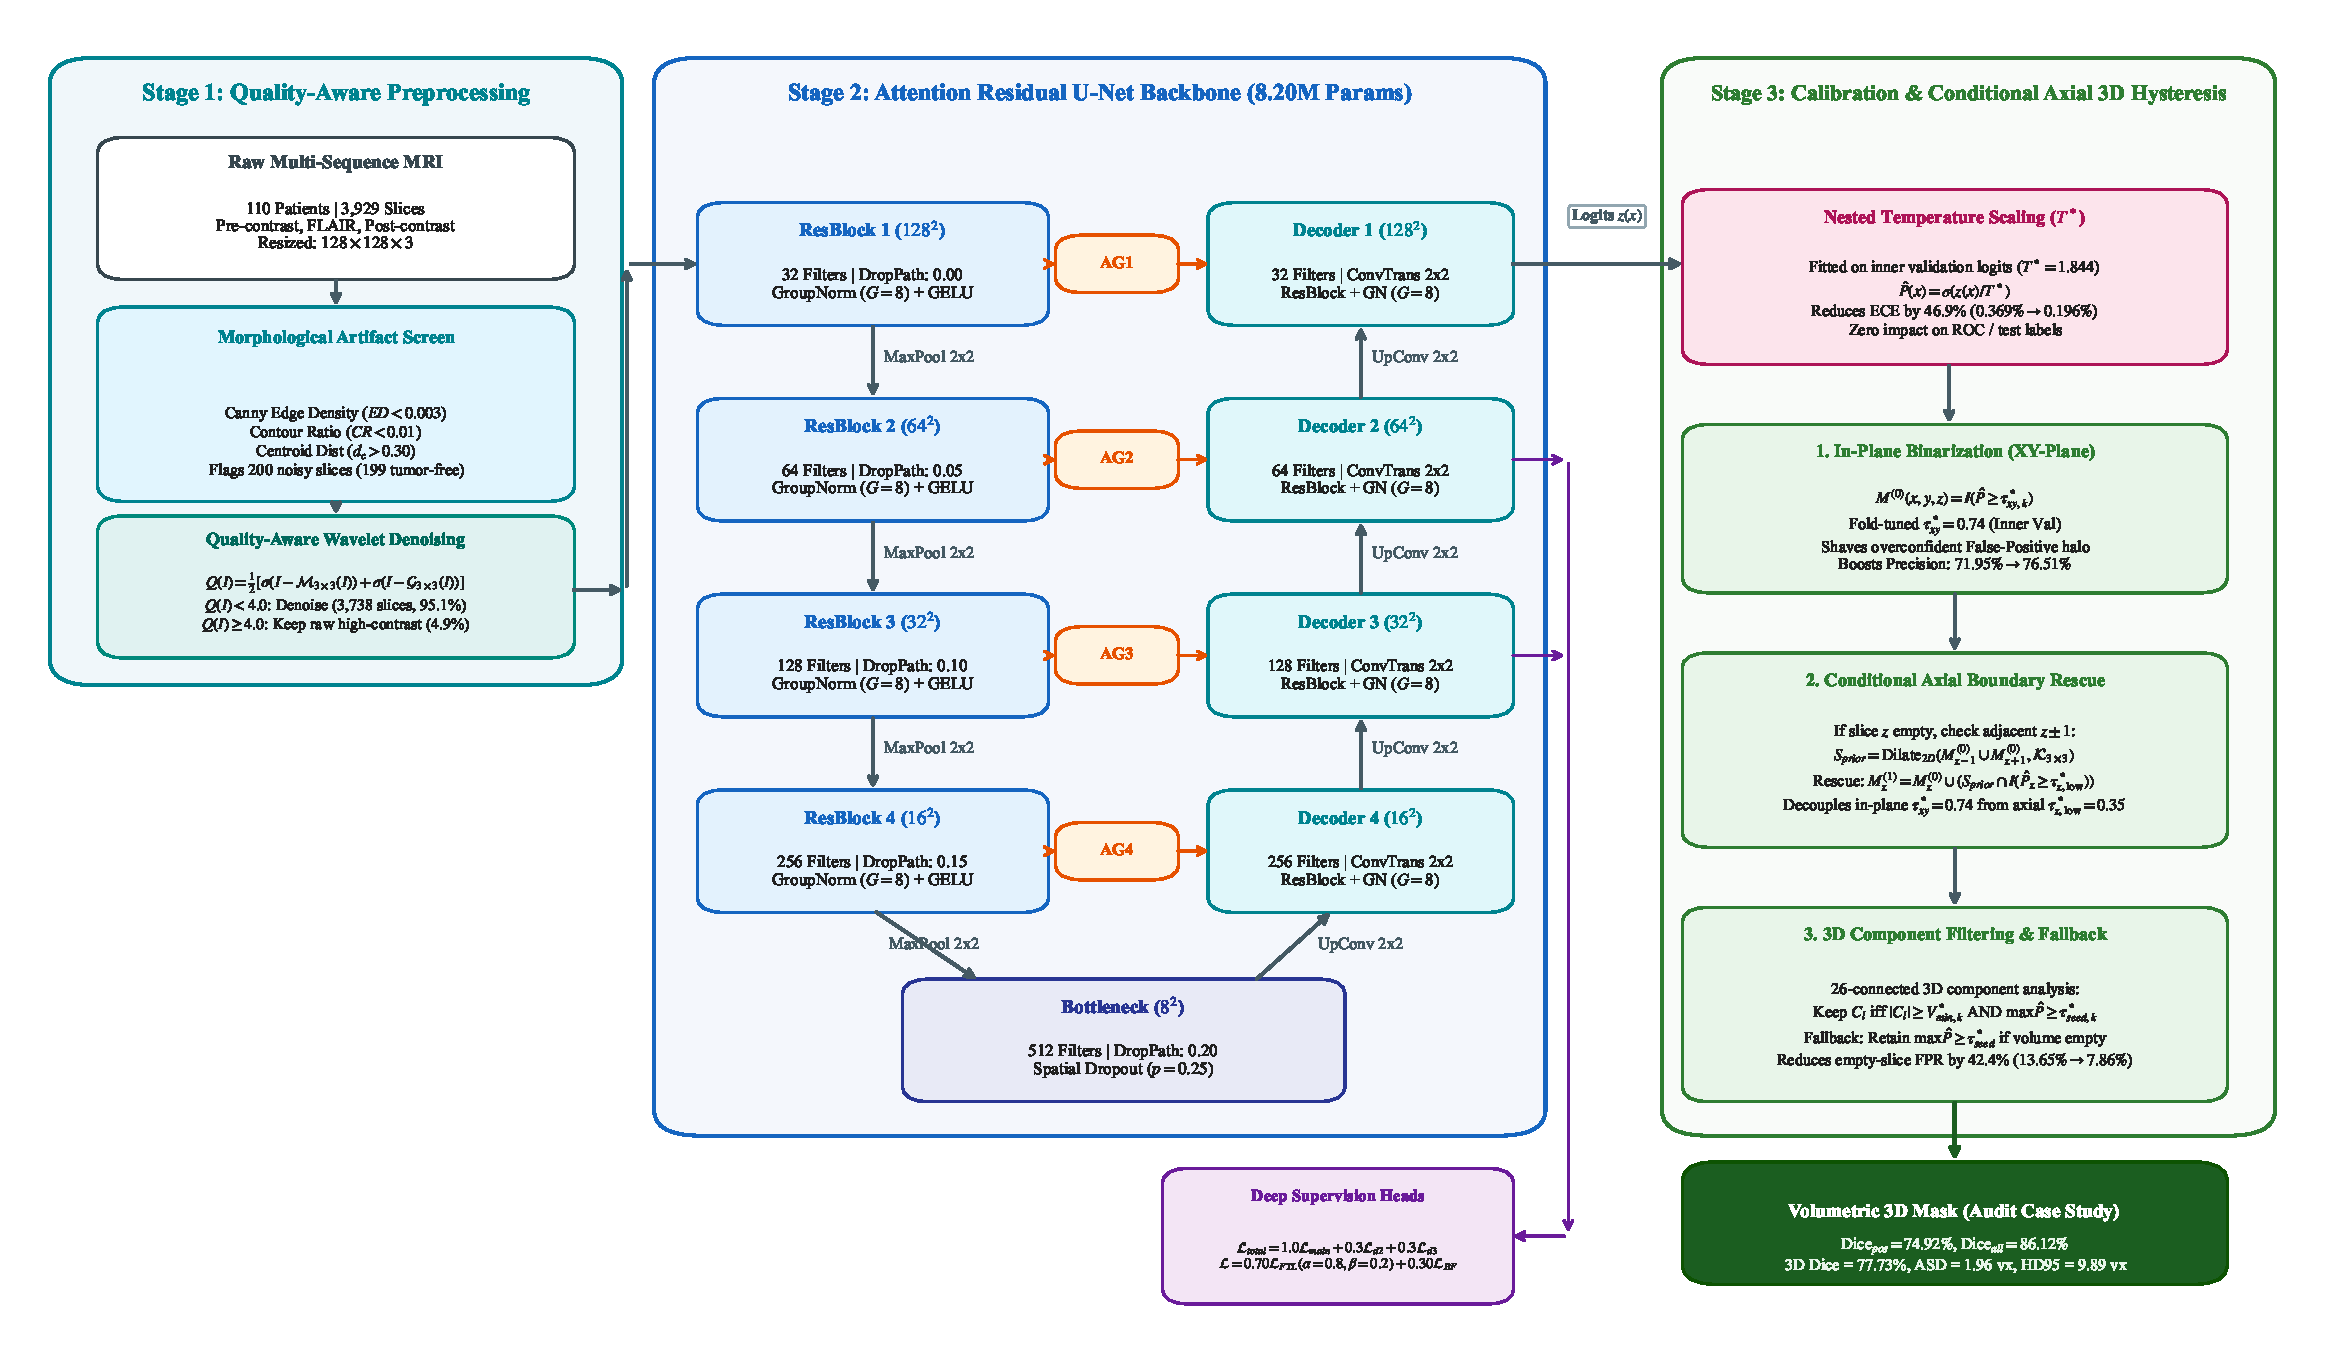
\includegraphics[width=0.98\textwidth]{Fig2.pdf}
\caption{End-to-end CAL-3DH processing pipeline showing Quality-Aware Preprocessing (Stage 1), the Attention Res-UNet backbone with Group Normalization ($G=8$), GELU, Stochastic Depth, and Deep Supervision (Stage 2), followed by Nested Temperature Scaling ($T^* = 1.844$) and Conditional Axial Z-Rescue Hysteresis (Stage 3)}
\label{fig:architecture_pipeline}
\end{figure}

\subsection{Attention Residual U-Net Architecture and Training Dynamics}
The segmentation backbone of CAL-3DH employs an Attention Residual U-Net (Attn Res-UNet) with deep supervision (Figure~\ref{fig:architecture_pipeline}). Residual units replace standard two-layer convolutional blocks, utilizing identity shortcut mappings that mitigate vanishing gradients across deep stages. Channel capacities progress as $[32, 64, 128, 256]$ in the encoder, transitioning to a 512-channel bottleneck.

To ensure numerical stability when training with small mini-batch sizes ($B=16$), all batch normalization layers are replaced with Group Normalization (GN)~\cite{wu2018group} using $G=8$ groups:
\begin{equation}
x_{\text{norm}} = \gamma \cdot \frac{x - \mu_{G}}{\sqrt{\sigma_{G}^2 + \epsilon}} + \beta
\end{equation}
where $\mu_{G}$ and $\sigma_{G}$ are computed independently across spatial coordinates and group channels. Feature non-linearities utilize Gaussian Error Linear Units (GELU)~\cite{hendrycks2016gaussian}:
\begin{equation}
\text{GELU}(x) = x \cdot \Phi(x) = x \cdot P(X \le x), \quad X \sim \mathcal{N}(0, 1)
\end{equation}
Regularization is reinforced via Stochastic Depth (DropPath)~\cite{huang2016deep} across residual branches:
\begin{equation}
\begin{aligned}
H &= \text{GELU}\left(\text{shortcut}(x) + \frac{b}{1-p}\mathcal{F}(x)\right), \\
b &\sim \text{Bernoulli}(1-p)
\end{aligned}
\end{equation}
with linear decay rates $p \in [0.00, 0.05, 0.10, 0.15]$ in the encoder stages and $p=0.20$ at the bottleneck.

In the decoder, additive attention gates~\cite{oktay2018attention} dynamically recalibrate intermediate feature representations before concatenation. Given spatial features $x^l$ and gating signal $g$, attention coefficients $\alpha^l \in [0, 1]$ are obtained via:
\begin{equation}
\alpha^l = \sigma\left(\psi^T \left(\text{GELU}\left(W_x^T x^l + W_g^T g + b_g\right)\right) + b_\psi\right)
\end{equation}
where linear projections $W_x$ and $W_g$ align channel dimensions, and $\sigma$ denotes the sigmoid activation. This gating suppresses background noise in peripheral brain regions while amplifying infiltrative tumor signals. Deep supervision auxiliary heads at decoders 2 and 3 provide intermediate gradients during backpropagation. The final network comprises exactly 8.20 million trainable parameters (8,202,005 parameters).

To address acute class imbalance (positive lesion pixels comprise less than $1.5\%$ of total voxels), networks were trained using a compound production loss combining Focal Tversky Loss (FTL)~\cite{salehi2017tversky,abraham2019novel} and Binary Focal Loss (BFL)~\cite{lin2017focal}:
\begin{equation}
\mathcal{L}_{\text{total}} = 0.70\,\mathcal{L}_{\text{FTL}} + 0.30\,\mathcal{L}_{\text{BF}}
\end{equation}
The Focal Tversky formulation is defined as:
\begin{equation}
\text{TI}(y, \hat{p}) = \frac{\sum_i y_i \hat{p}_i + \epsilon}{\sum_i y_i \hat{p}_i + \alpha \text{FN}(y, \hat{p}) + \beta \text{FP}(y, \hat{p}) + \epsilon}
\end{equation}
\begin{equation}
\mathcal{L}_{\text{FTL}} = (1 - \text{TI})^\gamma
\end{equation}
where $\gamma = 0.60$ (corresponding to $1/\gamma_{AK} = 0.60$, i.e., $\gamma_{AK} = 5/3$ in the focal Tversky parameterization of Abraham and Khan~\cite{abraham2019novel}), $\epsilon = 1.0$, and the voxel-level error components are defined as $\text{FN}(y, \hat{p}) = \sum_i y_i(1 - \hat{p}_i)$ and $\text{FP}(y, \hat{p}) = \sum_i (1 - y_i)\hat{p}_i$.

In this formulation, $\alpha = 0.80$ is the penalty weight assigned to \textbf{False Negatives (FN)}, while $\beta = 0.20$ weights \textbf{False Positives (FP)}. Heavily penalizing false negatives ($\alpha = 0.80 \gg \beta = 0.20$) prioritizes the detection of diffuse, low-contrast tumor boundaries, achieving high baseline Recall ($82.98\%$). However, this asymmetric penalty leads raw network probabilities to exhibit an intermediate-confidence false-positive halo surrounding lesions (raw Precision = $71.95\%$) and substantial probability miscalibration ($T^* = 1.844$). As detailed in Section~\ref{sec:calibration_hysteresis}, this peripheral false-positive halo is systematically eliminated in the CAL-3DH framework through nested calibration and conditional axial 3D Z-hysteresis filtering, elevating final Precision to $76.86\%$.

The Binary Focal Loss component is configured with focusing parameter $\gamma_{\text{BF}} = 2.0$ and label smoothing $\epsilon_{\text{LS}} = 0.02$. Auxiliary heads participate via multi-scale deep supervision:
\begin{equation}
\label{eq:deep_supervision}
\mathcal{L}_{\text{multi}} = 1.0\,\mathcal{L}_{\text{total}}^{(\text{main})} + 0.30\,\mathcal{L}_{\text{total}}^{(d2)} + 0.30\,\mathcal{L}_{\text{total}}^{(d3)}
\end{equation}
Optimization utilized the AdamW optimizer~\cite{loshchilov2019decoupled} with weight decay ($10^{-4}$) and a Cosine Annealing learning rate schedule featuring an 8-epoch linear warmup up to $\eta_{\max} = 3 \times 10^{-4}$, decaying to $\eta_{\min} = 10^{-6}$ over 100 epochs with early stopping patience of 20 epochs. Mini-batch size was fixed to 16. Stochastic data augmentation (random rotation $\pm 15^\circ$, scaling $0.90$--$1.10$, and elastic deformation with $\alpha=15, \sigma=3$) was active strictly during training. Horizontal flipping was intentionally excluded to preserve biological hemispheric asymmetry of gliomas. Validation and testing were performed in pure deterministic inference mode. All experiments were implemented in Python 3.11 with PyTorch 2.4 and CUDA 12.2 on an NVIDIA RTX 4090 GPU (24GB VRAM). A fixed global random seed ($42$) was enforced across all patient-grouped folds, weight initialization, and stochastic data augmentations to support computational reproducibility.

\subsection{Patient-Grouped 5-Fold Cross-Validation and Metric Definitions}
To prevent slice-level data leakage, 110 patients were partitioned into 5 balanced folds using stratified group splitting (stratified by patient-level mean tumor slice ratio). All slices from any given patient were assigned strictly to a single fold.

In each fold $k \in \{1, \dots, 5\}$, exactly 22 patients ($20\%$ of the 110-subject cohort, $\approx 786$ slices per fold) were set aside as an untouched outer test partition (\texttt{outer\_test}), strictly blinded and untouched during model training and tuning, and used solely to evaluate pre-specified pipeline configurations. The remaining 88 non-test patients were systematically partitioned in an $85\% / 15\%$ ratio into 75 training patients ($\approx 2,535$ clean slices per fold following artifact exclusion) utilized to optimize network parameters $\theta_k$, and an internal holdout partition (\texttt{inner\_val}) of 13 patients ($\approx 468$ slices per fold, 2,338 slices pooled across the 5 folds). This 13-patient \texttt{inner\_val} split serves as the independent validation split for early-stopping checkpoint selection, scalar temperature scaling ($T_k^*$), and hysteresis hyperparameter selection ($\tau_{xy,k}^*, \tau_{z,\mathrm{low},k}^*, V_{\min,k}^*, \tau_{\mathrm{seed},k}^*$). While reserving 13 patients specifically for inner calibration reduces the training pool from 88 to 75 subjects, this design is structured to prevent any hyperparameter, temperature ($T^*$), or threshold ($\tau^*$) leakage into the 22 held-out test patients.

Every test slice was evaluated strictly by the single dedicated model $\mathcal{M}_k(\cdot; \theta_k^*)$ trained for that fold:
\begin{equation}
\hat{Y}_i = \mathcal{M}_k(X_i; \theta_k^*), \quad \forall i \in \mathcal{D}_{\text{test}}^{(k)}
\end{equation}
This 1-to-1 patient-to-fold mapping eliminates ensemble averaging ambiguity: no soft blending or multi-model averaging was utilized.

To quantify the precise degree of optimistic bias induced by slice-level data leakage, a matched parallel 5-fold Random-Slice cross-validation control experiment was conducted concurrently. Under this control protocol, the 3,929 axial slices were randomly partitioned into five equal folds without patient identity grouping, allowing slices from all 110 patients (100\% patient overlap) to co-exist simultaneously across training, validation, and testing sets. Identical network architectures, learning rate schedules, loss formulations ($\alpha=0.8, \beta=0.2, \gamma=0.6$), and stopping criteria were strictly enforced to isolate the effect of patient-level data leakage from model capacity.

In MRI volumes containing large proportions of healthy slices, evaluation metrics must handle non-tumor slices without distortion. To audit the prevailing evaluation convention in prior brain MRI literature, we evaluate the common empty-slice scoring rule:
\begin{equation}
\text{Dice}(y, \hat{y}) = \begin{cases}
1.0, & \text{if } |y| = 0 \;\land\; |\hat{y}| = 0 \text{ (TN)} \\
0.0, & \text{if } |y| = 0 \;\land\; |\hat{y}| > 0 \text{ (FP)} \\
\frac{2|y \cap \hat{y}|}{|y| + |\hat{y}|}, & \text{if } |y| > 0
\end{cases}
\end{equation}
Three primary slice-level metrics are reported to comprehensively capture clinical utility: $\text{Dice}_{\text{pos}}$, calculated strictly over the 1,373 tumor-bearing slices ($|y| > 0$); $\text{Dice}_{\text{all}}$, computed over all 3,929 slices including healthy non-tumor tissue; and the empty-slice false-positive rate ($\text{FPR}_{\text{empty}}$), quantifying the percentage of healthy slices erroneously predicted to contain lesion voxels ($|\hat{y}| > 0$ when $|y| = 0$). In prior medical imaging literature, it has been conventional to assign $\text{Dice} = 1.0$ (TN) to true-negative empty slices. However, consistent with the general guidance in the \textit{Metrics Reloaded} framework~\cite{maierhein2024metrics} on handling empty reference slices, this convention induces severe metric inflation and dilution in volumetric cohorts dominated by negative slices, which we analytically formulate and quantify in Section~3.6. For 3D surface distance evaluation ($\text{HD}_{95}$ and $\text{ASD}$), when both predicted and reference volumes are empty ($y=0, \hat{y}=0$), distance is defined as $0.0\text{ voxels}$; when one volume is empty while the other contains foreground, a standard bounding-box diagonal penalty $\sqrt{128^2 + 128^2 + N_z^2}\text{ voxels}$ ($\approx 182.14\text{ voxels}$) is assigned.


\noindent\textbf{Pre-specified Primary Protocol vs.\ Post-Hoc Comparators.}
To isolate the specific benefit of conditional axial decoupling from general morphological post-processing, the primary four pipeline stages (Step~1 In-Plane Binarization, Step~2 Axial Z-Continuity Rescue, Step~3 3D Component Filtering, and Fallback) were pre-specified. Supplementary morphological comparators (Volume-Wise Largest-CC, Max-Confidence CC, Axial Z-Median Filtering, and Matched-Structure 3D Dilation) were subsequently conducted as post-hoc audit evaluations. In the Random-Slice regime, all 3,929 axial slices were partitioned into training (68\%, 2,672 slices), validation (12\%, 471 slices), and test (20\%, 786 slices) per fold; identically to the patient-grouped regime, artifact screening exclusion was strictly applied only to training folds to maintain perfectly matched training conditions (~2,535 clean slices per fold; inducing 0.00 pp change in test Dice, Table~\ref{tab:screening_audit}).

\noindent\textbf{Zero-Parameter Nearest-Slice Label-Copy Oracle and Inter-Slice Mask Continuity Index (MCI).}
To establish a zero-parameter anatomical reference baseline quantifying how much spatial overlap is available purely from contiguous spatial proximity without training any deep neural network, we formulate a zero-parameter nearest-slice label-copy oracle under the random-slice split regime. For each test slice $z \in Z_i^{\text{test}}$ belonging to subject $i$, the oracle identifies the nearest slice $z^* \in Z_i^{\text{train}}$ from the same subject present in the training partition:
\begin{equation}
z^* = \arg\min_{z' \in Z_i^{\text{train}}} |z - z'|
\end{equation}
The oracle assigns the ground-truth annotation of slice $z^*$ as its prediction $\hat{Y}_{i,z} = Y_{i,z^*}$; specifically, when test slice $z$ is flanked symmetrically by training slices at equidistant separation $z \pm k$, signed distance transform (SDT) interpolation is applied between the two neighbors, whereas when only a one-sided neighbor is available within buffer distance $k$, direct label copying is used. To evaluate the spatial range of anatomical leakage, we test buffer separation distances $k \in \{0, 1, 2, 3, 4, 5\}$ such that $|z - z^*| \ge k$.

Complementing the copy oracle, we define the intrinsic, model-free \textbf{Inter-Slice Mask Continuity Index} ($\text{MCI}_i$) for each patient $i$ as the average Dice overlap between consecutive true tumor-bearing slices $Z_i^+$:
\begin{equation}
\text{MCI}_i = \frac{1}{|Z_i^+| - 1} \sum_{z=1}^{|Z_i^+|-1} \text{Dice}(Y_{i,z}, Y_{i,z+1})
\end{equation}
$\text{MCI}_i$ quantifies the intrinsic inter-slice morphological continuity of each tumor volume, providing a model-free descriptor of intrinsic inter-slice label continuity to test whether geometric mask continuity alone explains per-patient neural network leakage inflation. To rigorously probe non-spatial representation mechanisms, we implement a supervised Appearance Fingerprint Probe (extracting a 17-dimensional texture vector exclusively from non-lesional brain parenchyma voxels where $Y=0$, classified via 1-NN cosine similarity), evaluate measurement invariance via odd-versus-even slice split-half reliability and two one-sided equivalence tests (TOST within $|\Delta r| < 0.25$), and evaluate ranking stability using tie-buffered Kendall's rank correlation coefficient $\tau_b$. Slice-level inflation heterogeneity is further modeled via a linear mixed-effects regression ($\Delta\text{Dice}_s \sim \text{ProbeCosineSim}_s + \Delta z_s + \log(\text{SliceTumorArea}_s) + (1 \mid \text{Patient})$) with Z-standardized predictors.

\subsection{Nested Temperature Scaling Calibration}
Because overlap losses yield uncalibrated probability estimates, raw network logits $z(x)$ were calibrated via post-processing temperature scaling~\cite{guo2017calibration}. Temperature parameter $T_k > 0$ was optimized strictly on inner validation logits by minimizing negative log-likelihood (NLL):
\begin{equation}
\begin{aligned}
\hat{T}_k^* = \arg\min_{T > 0} \sum_{j \in \mathcal{D}_{\text{val}}^{(k)}} \Big[ &-y_j \log \sigma(z_j / T) \\
&-(1 - y_j) \log \big(1 - \sigma(z_j / T)\big) \Big]
\end{aligned}
\end{equation}
Because temperature scaling applies a monotonic scalar transformation ($T_k > 0$), it preserves the relative ranking of logits while softening extreme confidence values. Expected Calibration Error (ECE) was calculated across $M = 15$ equally spaced probability bins:
\begin{equation}
\text{ECE} = \sum_{m=1}^M \frac{|B_m|}{N} \left| \text{acc}(B_m) - \text{conf}(B_m) \right|
\end{equation}
To quantify miscalibration within the clinically critical infiltrative margin region while preventing background dilution by easy non-tumor voxels, we define the active-bin calibration (overconfidence) gap across intermediate-probability bins $\mathcal{M}_{\text{active}} = \{m \mid \text{bin}_m \subseteq [0.2, 0.9]\}$, where $\text{conf}(B_m) > \text{acc}(B_m)$ across all active bins in Figure~\ref{fig:reliability_diagram}(a):
\begin{equation}
\text{Gap}_{\text{active}} = \frac{1}{|\mathcal{M}_{\text{active}}|} \sum_{m \in \mathcal{M}_{\text{active}}} \left( \text{conf}(B_m) - \text{acc}(B_m) \right)
\end{equation}
and evaluate the corresponding voxel-weighted active-bin Expected Calibration Error:
\begin{equation}
\text{ECE}_{\text{active}} = \frac{\sum_{m \in \mathcal{M}_{\text{active}}} |B_m| \left| \text{acc}(B_m) - \text{conf}(B_m) \right|}{\sum_{m \in \mathcal{M}_{\text{active}}} |B_m|}
\end{equation}
which directly measures infiltrative margin miscalibration and corresponds to the $36.14\%$ to $29.57\%$ reduction reported in Section~\ref{sec:calibration_results}.

The functional role of calibration in the CAL-3DH pipeline is practical rather than fundamental to multi-parameter volumetric post-processing. While a single in-plane threshold $\tau_{xy,k}^*$ could be mapped monotonically to an uncalibrated threshold $\tau_{\text{raw},k}^* = \sigma(T_k^* \operatorname{logit}(\tau_{xy,k}^*))$, CAL-3DH evaluates candidate 3D hysteresis grids ($\tau_{z,\mathrm{low}} \in \{0.35, 0.40, 0.45, 0.50\}$, $\tau_{\mathrm{seed}} \in \{0.70, 0.75\}$) across folds whose uncalibrated logit scales vary substantially ($T_k^* \in [1.520, 2.387]$); calibrating probabilities first aligns all folds onto a common probability scale and facilitates probability comparability across folds~\cite{guo2017calibration,mukhoti2020calibrating,jungo2019assessing} along ambiguous boundaries, providing a consistent probabilistic basis for evaluating candidate spatial rules across unseen test volumes.


\noindent\textbf{Remark 1 (Monotonic Calibration Invariance).}
\textit{Let $z(x) \in \mathbb{R}$ denote the predicted logit for voxel $x$, and let $g: \mathbb{R} \to [0, 1]$ be any strictly monotonically increasing calibration mapping (such as temperature scaling $g(z) = \sigma(z/T)$ with $T > 0$, or affine Platt scaling $g(z) = \sigma(az+b)$ with $a > 0$). For any spatial overlap metric $\mathcal{M}$ defined on binary segmentation masks and any decision threshold grid with discretization step $\delta\tau \to 0$, the optimal decision boundary satisfies $\tau_{\text{cal}}^* = g(\tau_{\text{raw}}^*)$ and the optimal segmented masks are strictly identical: $\hat{Y}_{\text{cal}}(x) = \hat{Y}_{\text{raw}}(x)$ for all $x$. Thus, post-hoc monotonic probability calibration strictly preserves voxel rank ordering and produces identical validation-optimized binary spatial overlap up to grid discretization step $\delta\tau$.}

\noindent\textbf{Exploratory Patient-Level Conformal Risk Control Safety Audit.}
To evaluate the downstream safety consequences of evaluation leakage beyond mean overlap metrics, we conduct an exploratory conformal safety audit under the split conformal risk control framework of Angelopoulos et al.~\cite{angelopoulos2024conformal}. To isolate the calibration protocol entirely from confounding model differences, evaluations are conducted on the \textbf{exact same single unified Patient-Grouped network}, comparing out-of-patient calibration ($\hat{\lambda}_{\text{out}}$ calibrated strictly on independent inner-validation subjects $\mathcal{D}_{\text{val}}^{(k)}$) against contaminated in-patient calibration ($\hat{\lambda}_{\text{in}}$ derived from training-set slices of the same fold, where calibration slices originate from patients whose representations were already memorized during training $\mathcal{D}_{\text{train}}^{(k)}$). Both calibrated thresholds are subsequently evaluated on the exact same genuinely unseen out-of-patient test subjects (\texttt{outer\_test}, $n=110$ across the five folds), isolating the specific impact of patient-identity leakage during the threshold calibration phase. Nominal $90\%$ tumor voxel coverage ($1 - \alpha = 0.90$) is evaluated under two formulations: (i) voxel-pooled 10th percentile calibration on foreground voxels, and (ii) patient-level Conformal Risk Control (CRC)~\cite{angelopoulos2024conformal} where the threshold $\hat{\lambda}$ is chosen to bound expected patient-level loss $\mathbb{E}[L_i(\lambda)] \le \alpha = 0.10$ for per-patient non-coverage loss $L_i(\lambda) = 1 - C_i(\lambda) = 1 - |\{x \in Y_i^+ \mid \hat{p}(x) \ge \lambda\}| / |Y_i^+|$. To evaluate finite-sample calibration stability beyond the $n_{\text{cal}} = 13$ inner-validation subjects per fold (which also participate in early stopping and scalar temperature fitting), we additionally perform 1,000 paired Monte Carlo resamplings drawing $n_{\text{cal}} = 30$ calibration subjects and $n_{\text{eval}} = 80$ evaluation subjects from the 110 out-of-fold test predictions.

\subsection{Conditional Axial Z-Continuity Rescue Algorithm (CAL-3DH)}\label{sec:calibration_hysteresis}
In 2D axial segmentation, high decision thresholds suppress false alarms but truncate apical and basal tumor margins, whereas low thresholds preserve boundaries at the expense of false alarms on healthy slices. CAL-3DH resolves this trade-off through a conditional axial z-continuity hysteresis algorithm operating across calibrated probabilities $\hat{P} = \sigma(z / \hat{T}_k^*)$. All post-processing hyperparameters were optimized strictly on internal validation splits (\texttt{inner\_val}, 13 patients): (1) scalar temperature $T_k \in [0.5, 4.0]$ via bounded scalar minimization of validation NLL; (2) planar threshold $\tau_{xy,k} \in [0.20, 0.90]$ with step $0.02$ maximizing validation $\text{Dice}_{\text{pos}}$; and (3) 3D spatial parameters via grid search over $\tau_{z,\mathrm{low}} \in \{0.35, 0.40, 0.45, 0.50\}$, $V_{\min} \in \{20, 50, 80\}$, and $\tau_{\mathrm{seed}} \in \{0.70, 0.75\}$ maximizing inner-validation slice-averaged positive Dice ($\text{Dice}_{\text{pos}}$):
\begin{enumerate}
    \item \textbf{In-Plane Planar Binarization:} Each slice is initially thresholded with fold-specific inner-validation threshold $\tau_{xy, k}^*$ ($0.62 \le \tau_{xy}^* \le 0.84$, mean: $0.74$):
    \begin{equation}
    M^{(0)}(x, y, z) = \mathbb{I}\left( \hat{P}(x, y, z) \ge \tau_{xy, k}^* \right)
    \end{equation}
    preserving horizontal tumor boundary fidelity and shaving the FP halo.
    \item \textbf{Z-Continuity Boundary Rescue:} For slices where $M^{(0)}$ detects zero (or near-zero, $< 10$ pixels) tumor tissue, adjacent slices $z-1$ and $z+1$ are inspected. If an adjacent slice contains a verified tumor ($\ge 20$ pixels), a dilated spatial footprint $\mathcal{S}_{\text{prior}}$ is projected onto slice $z$:
    \begin{equation}
    \mathcal{S}_{\text{prior}} = \text{Dilate}_{2D}\left(M^{(0)}_{z-1} \cup M^{(0)}_{z+1}, \mathcal{K}_{3\times 3}\right)
    \end{equation}
    Voxels within $\mathcal{S}_{\text{prior}}$ satisfying a relaxed axial threshold $\tau_{z,\mathrm{low}, k}^*$ (mean $\tau_{z,\mathrm{low}}^* = 0.35$, where $\tau_{z,\mathrm{low}}^* < \tau_{xy}^*$) are rescued:
    \begin{equation}
    M^{(1)}_z = M^{(0)}_z \cup \left( \mathcal{S}_{\text{prior}} \cap \mathbb{I}(\hat{P}_z \ge \tau_{z,\mathrm{low}, k}^*) \right)
    \end{equation}
    \item \textbf{3D Volumetric Suppression:} On the resulting 3D volume, 26-connected components $\{C_l\}$ are labeled. Components are discarded if their 3D volume is smaller than $V_{\min, k}^*$ (mean $V_{\min}^* = 38$ voxels) or their peak probability is below $\tau_{\mathrm{seed}, k}^*$ (mean $\tau_{\mathrm{seed}}^* = 0.70$):
    \begin{equation}
    \begin{aligned}
    \mathcal{C}_{\text{valid}} = \big\{ C_l \mid &|C_l| \ge V_{min, k}^* \;\land \\
    &\max_{v \in C_l} \hat{P}(v) \ge \tau_{seed, k}^* \big\}
    \end{aligned}
    \end{equation}
    \item \textbf{Fallback Safeguard:} To prevent small apical tumors from collapsing to empty volumes (which imposes maximal boundary distance penalties), if $\mathcal{C}_{\text{valid}} = \emptyset$, components with $\max \hat{P} \ge \tau_{\mathrm{seed}}^*$ are retained. This safeguard is active in both the 3D-filtered ablation (Step 1 + Step 3) and Full CAL-3DH.
\end{enumerate}

The candidate search lower bounds ($\tau_{z,\mathrm{low}} \ge 0.35$, $\tau_{\mathrm{seed}} \ge 0.70$) were grounded in explicit biophysical and calibration constraints: lowering $\tau_{z,\mathrm{low}}$ below $0.35$ encroaches upon the low-confidence background noise floor and triggers excessive false-positive bleeding into adjacent tumor-free slices (empirically verified on internal validation splits, where relaxing $\tau_{z,\mathrm{low}}$ to $0.25$--$0.30$ degrades specificity by inflating empty-slice false alarms without rescuing additional true boundary slices), whereas lowering the 3D component seed threshold $\tau_{\mathrm{seed}}$ below $0.70$ drops below the calibrated in-plane decision plateau ($\tau_{xy}^* \in [0.62, 0.84]$, mean $0.74$), violating the hysteresis requirement that every retained 3D lesion component must be anchored by at least one high-confidence core voxel. Notably, because the inner-fold tuned in-plane threshold satisfies $\tau_{xy,k}^* \in \{0.76, 0.82, 0.84\} \ge \tau_{\text{seed}}^* = 0.70$ in Folds~1, 3, and 4, the confident-seed requirement is automatically fulfilled by in-plane voxels in those folds; the seed criterion operates as an active constraint primarily in Folds~2 and 5 ($\tau_{xy,k}^* \in \{0.62, 0.68\}$) and during fallback for zero-prediction volumes. To isolate the specific benefit of conditional axial decoupling from general morphological post-processing, we benchmark CAL-3DH against five isotropic and morphological control baselines in Table~\ref{tab:method_comparison} and Table~\ref{tab:patient_3d_metrics}: (1) a Conventional Isotropic 3D Component Filter corresponding to Step~1 + Step~3 (26-connected volume filtering without axial $z$-rescue); (2) Matched-Structure 3D Dilation, an isotropic control sharing identical Stage~1 and Stage~3 hyperparameters ($\tau_{xy}^*, V_{\min}^*, \tau_{\text{seed}}^*$) but replacing axial-only $z \pm 1$ rescue in Stage~2 with isotropic 3D dilation across all three axes using a $3 \times 3 \times 3$ structuring element constrained by $\tau_{\text{low}}^*$; (3) Volume-Wise Largest Connected Component (Largest-CC), which retains solely the single largest 3D component per volume under 26-connectivity; (4) a $1 \times 1 \times 3$ Axial Z-Median filter enforcing through-plane median continuity; and (5) Conventional Isotropic 3D Hysteresis applying uniform 3D dual thresholds ($\tau_{\text{high}}, \tau_{\text{low}}$) across all three spatial dimensions. For Conventional Isotropic 3D Hysteresis, hyperparameters were systematically tuned over the identical inner-validation search grid: $\tau_{\text{high}} \in [0.50, 0.90]$ (step $0.02$), $\tau_{\text{low}} \in \{0.35, 0.40, 0.45, 0.50\}$ with $\tau_{\text{low}} < \tau_{\text{high}}$, 26-connectivity propagation across all three spatial dimensions, minimum component volume $V_{\min} \in \{20, 50, 80\}$ voxels, and fallback to high-threshold voxels if all components fall below $V_{\min}$, selecting the parameter set that maximized $\text{Dice}_{\text{pos}}$ on \texttt{inner\_val}.

\section{Results}
\subsection{Baseline Segmentation Performance}
Table~\ref{tab:baseline_performance} summarizes baseline Attn Res-UNet performance across all 3,929 out-of-fold test slices at fixed threshold $\tau = 0.50$. Ninety-five percent confidence intervals were computed via 10,000 patient-clustered bootstrap iterations~\cite{efron1994introduction}. The model achieved a positive-slice Dice of $73.96\%$ [95\% CI: $70.10\%$--$77.15\%$], an overall Dice of $82.02\%$ [95\% CI: $79.75\%$--$84.10\%$], an intersection-over-union ($\text{IoU}_{\text{pos}}$) of $63.97\%$, and an empty-slice false-positive rate of $13.65\%$.

\begin{table}[tbp]
\centering
\caption{Baseline out-of-fold performance at fixed $\tau = 0.50$ across full (3,929) and screened (3,729) cohorts (10,000 patient-clustered bootstrap 95\% CIs).}
\label{tab:baseline_performance}
\setlength{\tabcolsep}{8pt}
\small
\begin{tabular*}{\textwidth}{@{\extracolsep{\fill}}lcc}
\toprule
\textbf{Evaluation Metric} & \textbf{Full Cohort (3,929)} & \textbf{Screened Cohort (3,729)} \\
\midrule
$\text{Dice}_{\text{pos}}$ (\%) & 73.96 [70.10 -- 77.15] & 73.96 [70.10 -- 77.13] \\
$\text{Dice}_{\text{all}}$ (\%) & 82.02 [79.75 -- 84.10] & 82.21 [80.01 -- 84.27] \\
$\text{IoU}_{\text{pos}}$ (\%) & 63.97 [59.78 -- 67.89] & 63.97 [59.78 -- 67.88] \\
$\text{Precision}_{\text{pos}}$ (\%) & 71.95 [67.80 -- 75.80] & 71.95 [67.80 -- 75.80] \\
$\text{Recall}_{\text{pos}}$ (\%) & 82.98 [78.60 -- 86.70] & 82.98 [78.60 -- 86.70] \\
$\text{FPR}_{\text{empty}}$ (\%) & 13.65 (349 / 2556) & 13.41 (316 / 2357) \\
\bottomrule
\end{tabular*}
\end{table}

\begin{figure}[tbp]
\centering
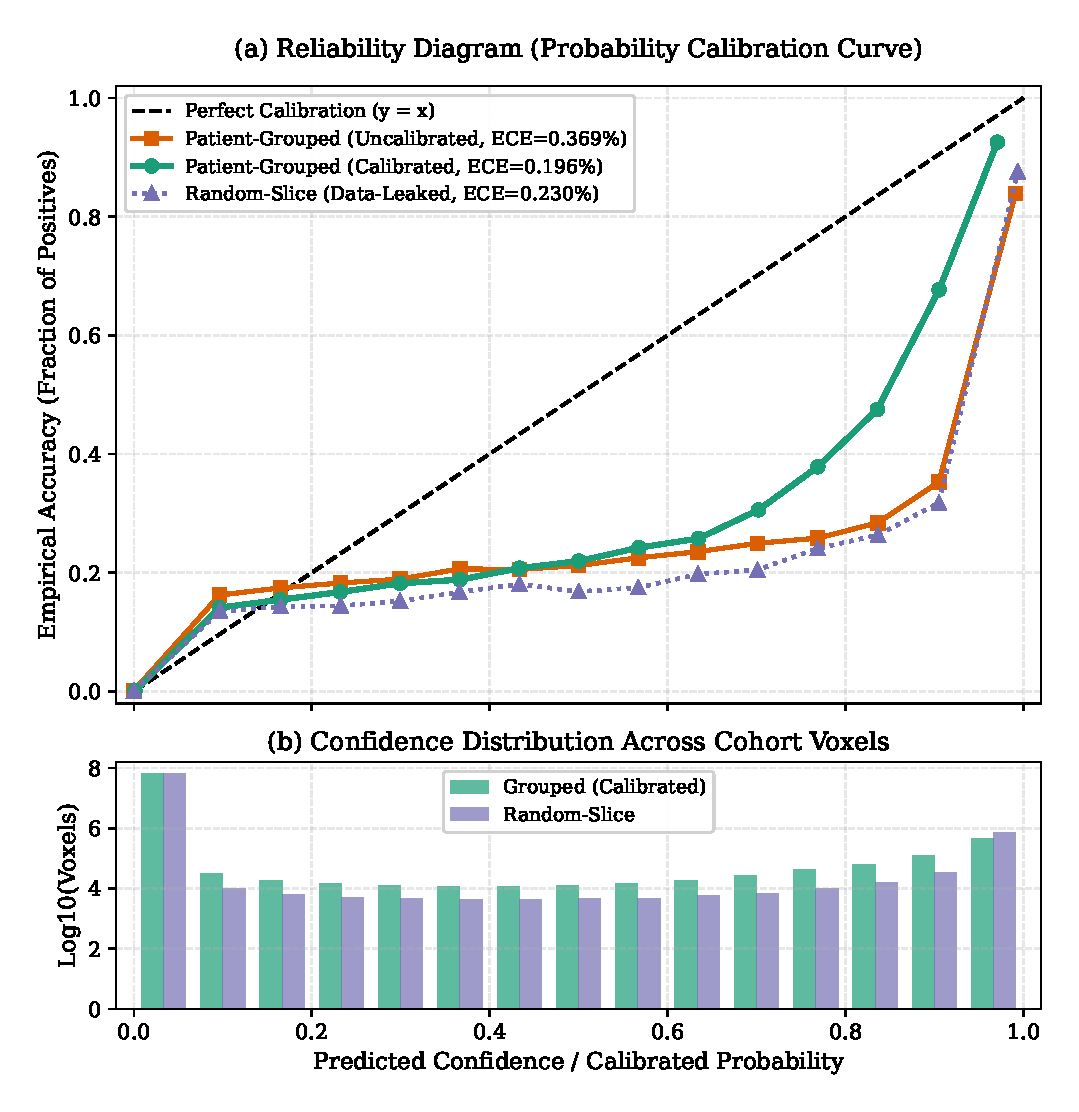
\includegraphics[width=0.98\textwidth]{Fig3.pdf}
\caption{Probability calibration and voxel confidence dynamics across 15 probability bins. (a) Reliability diagram comparing the uncalibrated patient-grouped model ($\text{ECE} = 0.369\%$), the temperature-calibrated model ($T^* = 1.844$, reducing pooled ECE by $46.9\%$ to $0.196\%$), and the data-leaked random-slice model against ideal diagonal calibration. (b) Logarithmic voxel frequency distribution across confidence bins for patient-grouped and random-slice regimes}
\label{fig:reliability_diagram}
\end{figure}

\subsection{Nested Temperature Scaling and Thresholding}
\label{sec:calibration_results}
Table~\ref{tab:calibration_folds} presents fold-by-fold calibration and threshold optimization results. Fitted optimal temperatures ranged from $T^* = 1.520$ to $2.387$ (mean $T^* = 1.844$). On untouched test sets, temperature scaling consistently reduced NLL from $0.0230$ to $0.0154$ ($-32.9\%$) and Brier score~\cite{brier1950verification} from $0.00375$ to $0.00338$ ($-9.9\%$). The mean per-fold ECE decreased from $0.372\%$ to $0.254\%$ (a $31.7\%$ relative reduction), while pooled cohort ECE dropped from $0.369\%$ to $0.196\%$ (a $46.9\%$ relative reduction), visually confirmed in Figure~\ref{fig:reliability_diagram}.

Crucially, the small absolute magnitude of cohort ECE ($0.369\%$) stems from voxel dilution: over $98.5\%$ of MRI voxels belong to background air and healthy, non-enhancing brain tissue ($y=0, \hat{p} \approx 0$, clearly reflected in the first bin of the logarithmic histogram in Figure~\ref{fig:reliability_diagram}(b) encompassing $>6 \times 10^7$ voxels). Within the clinically vital active probability bins corresponding to the ambiguous infiltrative tumor margins ($\hat{p} \in [0.2, 0.9]$ in Figure~\ref{fig:reliability_diagram}(a)), the raw uncalibrated network exhibits severe overconfidence, manifested by an Overconfidence Gap of $0.253$ ($25.3\%$, Section~\ref{sec:leakage_audit}). Nested temperature scaling ($T^* = 1.844$) contracts this margin overconfidence gap down to $0.200$ (a $20.9\%$ relative reduction), substantially shifting empirical confidence toward the ideal diagonal while active-margin weighted ECE decreases from $36.14\%$ to $29.57\%$ (and unweighted mean over active bins in $[0.2, 0.9]$ from $39.16\%$ to $37.87\%$). The corresponding training and validation convergence dynamics across folds are illustrated in Figure~\ref{fig:training_convergence}. In Figure~\ref{fig:training_convergence}(a), validation loss remains lower than training loss across epochs because heavy stochastic data augmentation, DropPath stochastic depth ($p \le 0.20$), and label smoothing ($\epsilon_{\text{LS}} = 0.02$) act as strong regularizers during training and are deactivated during deterministic validation; in contrast, in the random-slice regime (Figure~\ref{fig:training_convergence}(c)--(d)), validation soft overlap unnaturally surpasses training soft overlap by $23.76\text{ pp}$ ($85.49\%$ vs.\ $61.73\%$) due to subject memorization across contiguous slices.

\begin{table}[t]
\centering
\caption{Fold-by-fold nested calibration, threshold optimization, and out-of-fold performance.}
\label{tab:calibration_folds}
\setlength{\tabcolsep}{1.2pt}
\scriptsize
\begin{tabular*}{\textwidth}{@{\extracolsep{\fill}}ccccccccccccc}
\toprule
\textbf{Fold} & \shortstack{\textbf{Optimal} \\ $\mathbf{T^*}$} & \shortstack{\textbf{Inner} \\ $\mathbf{\tau_{xy}^*}$} & \shortstack{\textbf{Inner} \\ $\mathbf{\tau_{z,\mathrm{low}}^*}$} & \shortstack{\textbf{Inner} \\ $\mathbf{V_{\min}^*}$} & \shortstack{\textbf{Inner} \\ $\mathbf{\tau_{\mathrm{seed}}^*}$} & \multicolumn{2}{c}{\textbf{Outer ECE (\%)}} & \multicolumn{2}{c}{\textbf{Outer NLL}} & \multicolumn{3}{c}{\textbf{Outer Test $\text{Dice}_{\text{pos}}$ (\%)}} \\
\cmidrule(lr){7-8} \cmidrule(lr){9-10} \cmidrule(lr){11-13}
& & & & & & Raw & Calibrated & Raw & Calibrated & \shortstack{2D Base \\ ($\tau=0.50$)} & \shortstack{2D Nested \\ ($\tau_{xy}^*$)} & \shortstack{CAL-3DH \\ (Proposed)} \\
\midrule
1 & 2.019 & 0.76 & 0.35 & 50 & 0.70 & 0.354 & 0.153 & 0.0267 & 0.0159 & 77.02 & 77.00 & 77.26 \\
2 & 2.387 & 0.62 & 0.35 & 20 & 0.70 & 0.330 & 0.227 & 0.0191 & 0.0112 & 74.96 & 75.01 & 75.04 \\
3 & 1.649 & 0.82 & 0.35 & 80 & 0.70 & 0.391 & 0.367 & 0.0186 & 0.0141 & 79.39 & 81.91 & 82.39 \\
4 & 1.520 & 0.84 & 0.35 & 20 & 0.70 & 0.476 & 0.335 & 0.0325 & 0.0232 & 70.44 & 70.50 & 70.96 \\
5 & 1.644 & 0.68 & 0.35 & 20 & 0.70 & 0.308 & 0.186 & 0.0181 & 0.0127 & 68.15 & 68.61 & 69.01 \\
\midrule
Fold Mean & 1.844 & 0.74 & 0.35 & 38 & 0.70 & 0.372 & 0.254 & 0.0230 & 0.0154 & 73.99 & 74.61 & 74.93 \\
Pooled OOF & -- & -- & -- & -- & -- & 0.369 & 0.196 & 0.0230 & 0.0154 & 73.96 & 74.60 & 74.92 \\
\bottomrule
\end{tabular*}
\end{table}

\begin{figure}[tbp]
\centering
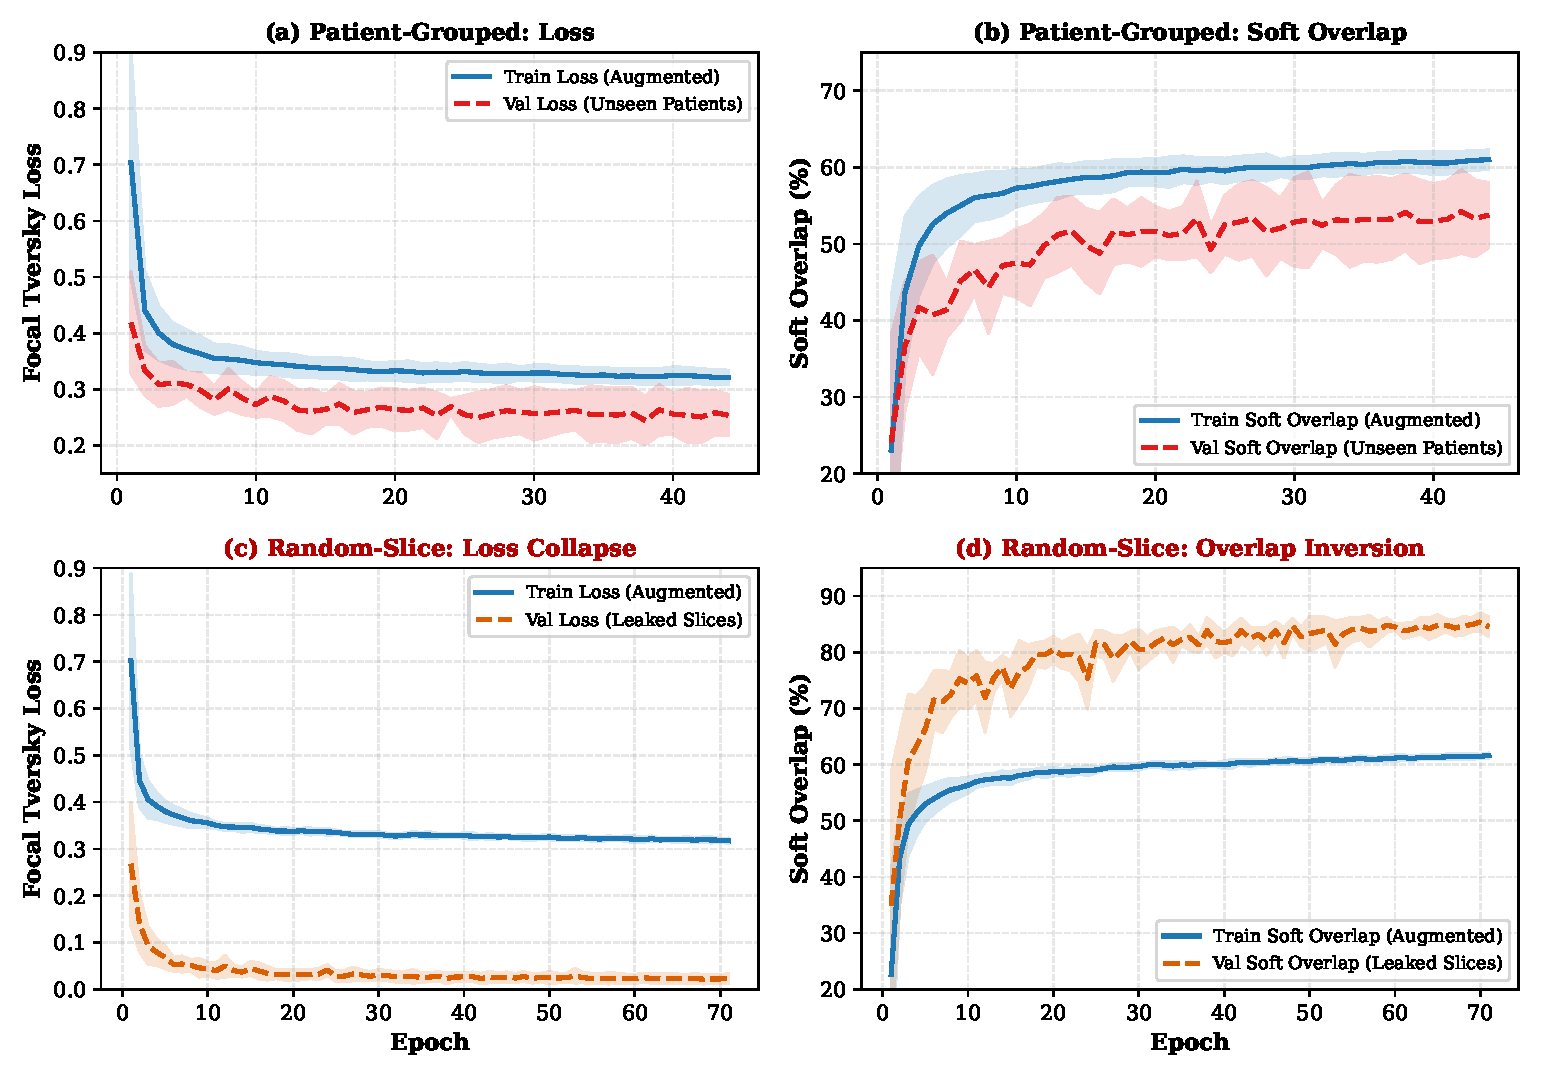
\includegraphics[width=0.92\textwidth]{Fig4.pdf}
\caption{Training and validation convergence dynamics across 5 folds under identical training hyperparameters. (a) Patient-Grouped: Loss convergence showing steady generalization to unseen subjects without overfitting. (b) Patient-Grouped: Soft overlap progression reaching stable plateau. (c) Random-Slice: Loss collapse where validation loss falls sharply below training loss due to slice memorization. (d) Random-Slice: Curve inversion where validation soft overlap exceeds training soft overlap by 23.76 pp (85.49\% vs. 61.73\%) across epochs}
\label{fig:training_convergence}
\end{figure}

\paragraph{Control Experiment: Disentangling Calibration from Spatial Post-Processing}
To isolate the independent contribution of temperature scaling calibration from downstream spatial post-processing, we conducted a matched control experiment tuning and evaluating the complete multi-step 3D hysteresis pipeline directly on uncalibrated logits ($T=1.0$) across all five folds under the identical inner-validation search grid and nested cross-validation protocol. On untouched test sets, uncalibrated 3D hysteresis achieves $\text{Dice}_{\text{pos}} = 74.90\%$, $\text{Dice}_{\text{all}} = 85.76\%$, $\text{FPR}_{\text{empty}} = 8.41\%$ ($215 / 2,556$ empty slices), and patient 3D volumetric Dice of $77.77\%$. In patient-level paired Wilcoxon signed-rank comparisons against temperature-calibrated CAL-3DH ($74.92\%$, 3D Dice $77.73\%$), differences in spatial overlap are negligible and statistically non-significant, with positive-slice overlap ($\Delta\text{Dice}_{\text{pos}} = -0.01\text{ pp}$, 95\% CI: $[-0.11, +0.11]\text{ pp}$, paired Wilcoxon $W = 142.0, p = 0.1437$) and 3D Dice ($\Delta\text{3D Dice} = -0.04\text{ pp}$, 95\% CI: $[-0.15, +0.07]\text{ pp}$, $p = 0.3177$) falling strictly within a $\pm 0.50\text{ pp}$ post-hoc equivalence margin (while $\Delta\text{Dice}_{\text{all}}$ spans $[-0.02, +0.74]\text{ pp}$ due to empty-slice false-alarm shifts). This empirical check confirms Remark~1 that temperature scaling does not function as an artificial spatial mask expander; rather, its vital methodological utility resides in uncertainty regularization (reducing active-margin ECE by $18.2\%$, cohort ECE by $46.9\%$, and Brier score by $9.9\%$) and standardizing heterogeneous raw logit scales across folds ($T_k^* \in [1.520, 2.387]$) onto an interpretable probability scale. Single-parameter temperature scaling ($T^*=1.844$) cannot eliminate the positive logit bias induced by asymmetric Focal Tversky weighting ($\alpha=0.80 \gg \beta=0.20$).

In contrast, fitting a two-parameter Platt/affine model $\hat{P} = \sigma(a_k z + b_k)$ on inner validation logits yields negative intercepts ($b_k \in [-1.68, -0.42]$, mean $-1.04$; $a_k \in [0.395, 0.615]$) that directly compensate for this prior shift. On outer test evaluation, two-parameter affine Platt scaling contracts weighted active-bin ECE from $36.14\%$ to $8.46\%$ (and unweighted active-bin ECE from $39.16\%$ to $9.12\%$) and the active-bin overconfidence gap to $7.59\%$ ($0.076$) (pooled ECE $0.130\%$, Brier score $0.00294$). In accordance with Remark~1 (Monotonic Calibration Invariance), strictly monotonic logit scaling ($a_k > 0$) ensures that validation-tuned binary segmentation masks remain identical ($\Delta\text{Dice}_{\text{pos}} = 0.00\text{ pp}$).

\noindent\textbf{Single-Model Patient-Level Conformal Risk Control Safety Audit.}
Evaluating patient-level coverage across all $n=110$ clinical subjects on the single Patient-Grouped model demonstrates that honest out-of-patient calibration achieves $85.74\% \pm 21.34\%$ mean ($94.29\%$ median, IQR: $[82.98\%, 98.94\%]$) patient-level test coverage. With only $n_{\text{cal}} = 13$ inner-validation subjects per fold, the finite-sample correction in split conformal theory ($1/(n_{\text{cal}}+1) \approx 7.1\%$) relative to $\alpha = 10\%$ is non-negligible, and a small tail of difficult low-contrast lesions pulls down the arithmetic mean (whereas the patient median reaches $94.29\%$). In repeated paired Monte Carlo resamplings with larger calibration cohorts (sampling $n_{\text{cal}} = 30$ calibration subjects and $n_{\text{eval}} = 80$ unseen evaluation subjects from the 110 out-of-fold test predictions across 1,000 Monte Carlo trials, where $1/(n_{\text{cal}}+1) \approx 3.2\%$), honest out-of-patient calibration achieves $90.08\% \pm 1.86\%$ coverage under the calibration 10th percentile threshold (and $90.21\% \pm 1.88\%$ under the finite-sample corrected CRC formula; 95\% empirical resampling interval: $[86.43\%, 93.79\%]$), closely matching nominal $90\%$ coverage. In contrast, contaminated calibration on same-patient training slices yields an empirical coverage of only $81.38\% \pm 2.75\%$ [95\% empirical resampling interval: $75.99\%, 86.86\%$], demonstrating a substantial paired coverage deficit of $-8.70\text{ pp}$ [95\% empirical resampling interval: $-12.72, -4.37\text{ pp}$] that mirrors the 5-fold cross-validation mean deficit ($-8.78 \pm 4.71\text{ pp}$). Explicitly optimizing the threshold under patient-level Conformal Risk Control (CRC)~\cite{angelopoulos2024conformal} to bound expected patient loss $\mathbb{E}[L_i(\lambda)] \le 0.10$ elevates mean patient-level test coverage to $87.69\% \pm 19.18\%$ (median $95.29\%$). In sharp contrast, calibrating conformal thresholds on in-sample training-patient slices (where training patient identities overlap with calibration slices) causes an empirical test coverage deficit on unseen clinical subjects, dropping mean patient coverage to $76.96\% \pm 22.46\%$ (median $85.87\%$, IQR: $[66.48\%, 92.92\%]$). Because each fold applies a shared calibration threshold, the primary summary statistic is the 5-fold mean deficit ($-8.78 \pm 4.71\text{ pp}$ across the 5 folds; fold-level drops: $-7.66, -16.18, -9.55, -3.32$, and $-7.22\text{ pp}$; all 5/5 folds negative, two-sided exact sign test $p = 0.0625$, one-sided $p = 0.0313$), while the 110-patient bootstrap interval ($-8.78\text{ pp}$ [95\% CI: $-11.09, -6.44\text{ pp}$]) reflects conditional dispersion across individual subjects (with patient-level coverage dropping from $85.74\%$ to $76.96\%$). This demonstrates that calibrating conformal thresholds on training-patient slices (violating calibration-test subject independence) induces substantial under-coverage on unseen patients, compromising formal conformal safety in prospective clinical AI deployment~\cite{angelopoulos2024conformal}.

\subsection{Quantification of Optimism Bias (\texorpdfstring{$\Delta\text{Optimism}$}{Delta Optimism})}
\label{sec:optimism_bias}
To rigorously disentangle sources of performance overestimation, we quantified the empirical difference between nested inner-fold thresholding and pooled test threshold sweeping (Figure~\ref{fig:threshold_sensitivity}). When decision thresholds were selected strictly on independent inner validation partitions (mean calibrated $\tau_{xy}^* = 0.74$, corresponding to raw uncalibrated threshold $0.86$), the model achieved an out-of-fold test $\text{Dice}_{\text{pos}}$ of $74.60\%$ [95\% CI: $70.45\%$--$78.08\%$]. Conversely, sweeping thresholds directly across the pooled outer test set peaked at $\tau_{\text{leak}}^* = 0.76$ (raw threshold $0.88$), yielding an apparent $\text{Dice}_{\text{pos}}$ of $74.66\%$. The resulting empirical optimism bias is:
\begin{equation}
\Delta\text{Optimism} = 74.66\% - 74.60\% = +0.063\text{ pp}
\end{equation}

This modest optimism bias ($+0.063\text{ pp}$) contrasts sharply with the massive $+8.79\text{ pp}$ inflation generated by slice-level data leakage (Section~\ref{sec:leakage_audit}). A likely contributor to artificial performance inflation in prior literature is within-patient inter-slice correlation across contiguous slices, whereas nested inner-fold thresholding represents an essential methodological best practice. Because the Dice plateau is remarkably stable across calibrated probabilities $\hat{P} \in [0.68, 0.85]$ (Figure~\ref{fig:threshold_sensitivity}), the empirical risk of post-hoc threshold tuning is negligible. This plateau stability indicates that transitioning from the default, suboptimal threshold ($\tau=0.50$) to the nested optimal threshold ($\tau_{xy}^* = 0.74$) legitimately captures $+0.64\text{ pp}$ in $\text{Dice}_{\text{pos}}$ ($73.96\%$ to $74.60\%$), a $+2.43\text{ pp}$ jump in overall $\text{Dice}_{\text{all}}$ ($82.02\%$ to $84.45\%$), and a $24.9\%$ relative reduction in empty-slice false alarms ($349$ to $262$ slices) with zero test partition snooping.

\begin{figure}[tbp]
\centering
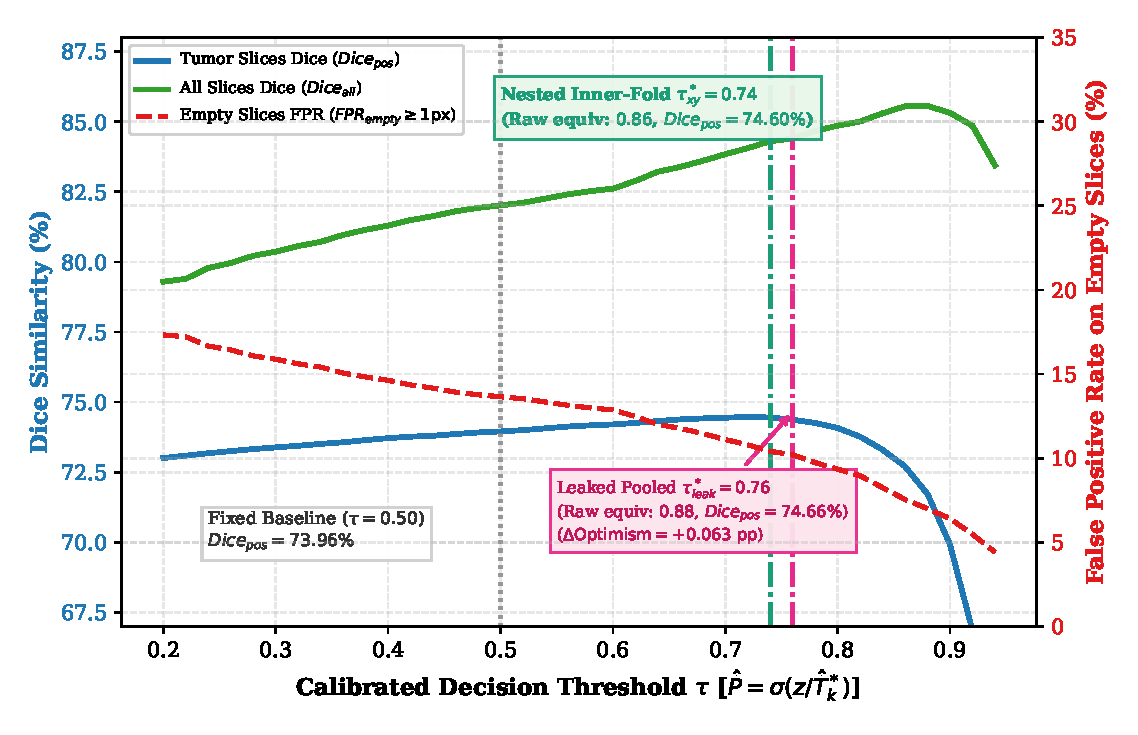
\includegraphics[width=\columnwidth]{Fig5.pdf}
\caption{Decision threshold sensitivity analysis on out-of-fold predictions plotted across calibrated probabilities $\hat{P} = \sigma(z/\hat{T}_k^*)$. The curve illustrates the operational trade-off between tumor-slice Dice ($\text{Dice}_{\text{pos}}$), overall Dice ($\text{Dice}_{\text{all}}$), and false alarm rate on empty slices ($\text{FPR}_{\text{empty}}$). Vertical markers denote the standard baseline ($\tau = 0.50$), the nested inner-fold calibrated threshold ($\tau_{xy}^* = 0.74$, corresponding to raw uncalibrated threshold $0.86$), and the post-hoc leaked threshold ($\tau_{\text{leak}}^* = 0.76$, raw equivalent $0.88$)}
\label{fig:threshold_sensitivity}
\end{figure}

\subsection{CAL-3DH Performance and Conditional Axial Z-Continuity Rescue Ablation}
In clinical volumetric FLAIR protocols where $65.05\%$ of axial slices are entirely tumor-free ($2,556 / 3,929$ slices), the primary clinical advantage of CAL-3DH lies in eliminating \textbf{148 false alarm slices relative to the baseline ($-42.4\%$, dropping from 349 to 201 slices)} and \textbf{61 fewer false alarm slices compared to 2D Nested ($-23.3\%$ additional relative reduction, from 262 to 201 slices)}. This selective pruning propels all-slice mean Dice ($\text{Dice}_{\text{all}}$) by $+4.10\text{ pp}$ ($+5.00\%$ relative gain) over baseline and $+1.67\text{ pp}$ over 2D Nested ($p < 0.0001$, patient-level paired Wilcoxon signed-rank test).

Crucially, unlike uniform-threshold 3D hysteresis without conditional empty-slice gating, which propagates false positives across slices on clinical 2D axial brain MRI acquisitions (where physical slice thickness and through-plane $z$-spacing are typically 4--6~mm vs.\ $\sim$1~mm in-plane prior to raster export), CAL-3DH preserves high-fidelity planar boundaries while recovering discontiguous apical and basal slices via confident 2D spatial seeds. Consequently, positive-slice Dice reaches $74.92\%$ [95\% CI: $70.82\%$--$78.39\%$], uniformly improving across all five cross-validation folds simultaneously (Table~\ref{tab:calibration_folds}).

To disentangle the specific biophysical contributions of each algorithmic component in Stage~3, Table~\ref{tab:method_comparison} details the step-by-step ablation across all 3,929 out-of-fold test slices:

\begin{enumerate}
\item \textbf{Step 1 Only (2D Nested Thresholding, $\tau_{xy}^*$):} Raising the in-plane decision threshold from $0.50$ to the calibrated inner-fold optimum $\tau_{xy}^* = 0.74$ elevates $\text{Dice}_{\text{pos}}$ from $73.96\%$ to $74.60\%$ and improves Precision from $71.95\%$ to $76.51\%$, reducing empty-slice false alarms by $24.9\%$ ($349$ to $262$ slices). However, it leaves missed apical/basal boundary slices unaddressed ($0 / 220$ rescued).
\item \textbf{Step 1 + Step 2 (+ Axial Z-Continuity Rescue, $\tau_{z,\mathrm{low}}^*$):} Activating axial continuity rescue ($\tau_{z,\mathrm{low}}^* = 0.35$ on slices adjacent to confident 2D seeds) boosts Recall from $80.14\%$ to $80.62\%$, elevates boundary slice Dice from $29.85\%$ to $30.39\%$, and successfully rescues $4$ previously completely missed apical boundary slices ($4 / 220$, $1.82\%$). Because low-threshold propagation can expand into adjacent slices, empty-slice false alarms slightly increase to $291$ slices ($11.38\%$) in the absence of volume filtering.
\item \textbf{Step 1 + Step 3 (+ 3D Component Filtering, $V_{\min}^*, \tau_{\mathrm{seed}}^*$):} Enforcing 3D connected-component volume filtering ($V_{\min}^* = 38$ voxels, $\tau_{\mathrm{seed}}^* = 0.70$) without Z-rescue aggressively suppresses spurious noise, dropping empty-slice false alarms to $176$ slices ($6.89\%$) and increasing $\text{Dice}_{\text{all}}$ to $86.66\%$ and Precision to $77.34\%$. However, without Z-rescue, missed boundary slices remain unrecovered ($0 / 220$).
\item \textbf{Full CAL-3DH (Step 1 + Step 2 + Step 3 + Fallback):} Combining both steps harmonizes the operational sensitivity-specificity trade-off through a complementary dual mechanism. Relative to \textbf{Step~1 + Step~2} (axial Z-rescue alone, Row~3: $\text{Dice}_{\text{pos}} = 74.88\%$, $\text{Dice}_{\text{all}} = 83.81\%$, $\text{FPR}_{\text{empty}} = 11.38\%$), adding 3D connected-component volume filtering (Step~3) retains all $4$ rescued apical boundary slices while yielding a modest $+0.04\text{ pp}$ gain in $\text{Dice}_{\text{pos}}$ ($74.88\%$ to $74.92\%$) and $+0.09\text{ pp}$ in boundary Dice ($30.39\%$ to $30.48\%$), while crucially eliminating \textbf{90 false-alarm slices} ($291 \to 201$ slices; a $-3.52\text{ pp}$ or $-30.9\%$ relative reduction in $\text{FPR}_{\text{empty}}$ from $11.38\%$ to $7.86\%$) and boosting all-slice mean Dice ($\text{Dice}_{\text{all}}$) by $+2.31\text{ pp}$ ($83.81\%$ to $86.12\%$), justifying Step~3 primarily on volumetric specificity grounds. Conversely, relative to \textbf{Step~1 + Step~3 (3D Component Filter)} (Row~4: $\text{Dice}_{\text{pos}} = 74.64\%$, $\text{Dice}_{\text{all}} = 86.66\%$, $\text{FPR}_{\text{empty}} = 6.89\%$), incorporating axial Z-continuity rescue (Step~2 in CAL-3DH) improves positive-slice Dice by $+0.28\text{ pp}$ ($74.64\%$ to $74.92\%$, patient-level paired Wilcoxon $W = 1.0, p = 0.0004$; 95\% CI: $[+0.12, +0.51]\text{ pp}$) and boundary-slice Dice by $+0.63\text{ pp}$ ($29.85\%$ to $30.48\%$). Specifically, relative to the 2D baseline ($\tau=0.50$), axial recovery rescues 4 polar boundary slices that were completely missed ($4/220$ in Table~\ref{tab:method_comparison}), whereas relative to Step~1 + Step~3 (where higher in-plane threshold $\tau_{xy}^*=0.74$ and small component filtering zero out 6 additional low-contrast boundary slices), it rescues a total of 10 boundary slices from zero detection, at the trade-off of 25 additional empty-slice false alarms ($176 \to 201$ slices; $\text{FPR}_{\text{empty}} = 6.89\%$ to $7.86\%$). In patient-level paired testing, exactly 17 patients exhibit non-zero paired differences between CAL-3DH and Step~1 + Step~3 ($W = 1.0, p_{\text{Holm}} = 0.0011$; 16 positive, 1 negative, and 93 identical; mean paired gain $+1.90\text{ pp}$ across the 17 affected patients). Crucially, on detected volumes ($n=109$), CAL-3DH and Step~1 + Step~3 are virtually indistinguishable in 3D surface metrics ($\text{ASD}: 1.96 \pm 3.58$ [median $0.61$] vs.\ $1.95 \pm 3.58$ [median $0.59$] voxels; $\text{HD}_{95}: 9.89 \pm 14.50$ [median $2.24$] vs.\ $9.88 \pm 14.49$ [median $2.24$] voxels; cohort-wide penalized $n=110$: $\text{ASD}$ $3.60 \pm 17.49$ vs.\ $3.59 \pm 17.49$, $\text{HD}_{95}$ $11.46 \pm 21.83$ vs.\ $11.44 \pm 21.81$ voxels) and global 3D volumetric Dice ($77.73\%$ vs.\ $77.75\%$, $p_{\text{Holm}} = 0.0211$ reflecting a negligible $-0.02\text{ pp}$ difference). Thus, incorporating conditional axial z-rescue (Step~2) provides localized apical margin restoration across 17 volumes ($+0.28\text{ pp}$ slice / $+0.29\text{ pp}$ patient $\text{Dice}_{\text{pos}}, p_{\text{Holm}} = 0.0011$) without altering global 3D surface distances, at the trade-off of 25 additional empty-slice false alarms ($176 \to 201$). Comparing planar versus 3D structuring elements (\textbf{Matched-Structure 3D Dilation}, Row~5) demonstrates that replacing $3\times 3$ planar dilation with $3\times 3\times 3$ 3D dilation yields negligible overlap change ($\Delta\text{Dice}_{\text{pos}} = -0.04\text{ pp}$, paired $W = 0.0, p_{\text{Holm}} = 0.3173$), with the difference falling strictly within the post-hoc equivalence margin of $\pm 0.50\text{ pp}$.
\end{enumerate}

\begin{table}[tbp]
\centering
\caption{Comprehensive ablation and benchmark comparison across 2D baselines, isotropic dilation controls, morphological heuristics, and CAL-3DH (all 3,929 out-of-fold test slices, 5 folds pooled). Boundary Dice evaluated exclusively across the 220 ground-truth lesion transition slices. Rescued indicates polar boundary slices transitioning from zero baseline prediction to non-zero true-positive overlap. FP Comps is mean false-positive 3D connected components per patient volume.}
\label{tab:method_comparison}
\setlength{\tabcolsep}{2.5pt}
\renewcommand{\arraystretch}{1.08}
\scriptsize
\resizebox{\textwidth}{!}{%
\begin{tabular}{lcccccccc}
\toprule
\textbf{Configuration / Ablation Stage} & \shortstack{$\mathbf{\text{Dice}_{\text{pos}}}$ \\ \textbf{(\%)}} & \shortstack{$\mathbf{\text{Dice}_{\text{all}}}$ \\ \textbf{(\%)}} & \shortstack{\textbf{Precision} \\ \textbf{(\%)}} & \shortstack{\textbf{Recall} \\ \textbf{(\%)}} & \shortstack{$\mathbf{\text{FPR}_{\text{empty}}}$ \\ \textbf{\% (count)}} & \shortstack{\textbf{Boundary} \\ \textbf{Dice (\%)}} & \shortstack{\textbf{Rescued} \\ \textbf{(/220)}} & \shortstack{\textbf{FP Comps} \\ \textbf{/ Pat}} \\
\midrule
\shortstack[l]{(1) 2D Baseline \\ \phantom{(1) }($\tau = 0.50$)} & 73.96 & 82.02 & 71.95 & \textbf{82.98} & 13.65 (349 / 2556) & 29.68 & 0 / 220 & 3.95 \\
\shortstack[l]{(2) Step 1: 2D Nested \\ \phantom{(2) }($\tau_{xy}^* = 0.74$)} & 74.60 & 84.45 & 76.51 & 80.14 & 10.25 (262 / 2556) & 29.85 & 0 / 220 & 3.07 \\
\shortstack[l]{(3) Step 1 + Step 2 \\ \phantom{(3) }(+ Axial Z-Rescue, $\tau_{z,\mathrm{low}}^*$)} & 74.88 & 83.81 & 75.82 & 80.62 & 11.38 (291 / 2556) & 30.39 & \textbf{4 / 220} & 3.24 \\
\shortstack[l]{(4) Step 1 + Step 3 (3D Component Filter) \\ \phantom{(4) }(26-conn., $V_{\min}^* = 38$)} & 74.64 & \textbf{86.66} & \textbf{77.34} & 79.45 & \textbf{6.89 (176 / 2556)} & 29.85 & 0 / 220 & 0.85 \\
\shortstack[l]{(5) Matched-Structure 3D Dilation \\ \phantom{(5) }(Isotropic 3D Dual-Dilation)} & 74.88 & 86.01 & 76.62 & 79.82 & 8.02 (205 / 2556) & 30.42 & \textbf{4 / 220} & 0.86 \\
\shortstack[l]{(6) Step 2 + Largest-CC \\ \phantom{(6) }(Axial Z-Rescue + Largest-CC)} & 74.24 & 89.39 & 76.20 & 78.93 & 2.46 (63 / 2556) & 30.12 & 0 / 220 & \textbf{0.03} \\
\shortstack[l]{(7) Volume-Wise Largest-CC \\ \phantom{(7) }(Single Largest 3D Component)} & 74.00 & 89.64 & 75.51 & 78.68 & \textbf{1.96 (50 / 2556)} & 29.62 & 0 / 220 & \textbf{0.03} \\
\shortstack[l]{(8) $1 \times 1 \times 3$ Axial Z-Median \\ \phantom{(8) }(Through-Plane Median Filter)} & 73.88 & 86.85 & 76.53 & 77.79 & 6.18 (158 / 2556) & 29.54 & 1 / 220 & 1.22 \\
\shortstack[l]{(9) Conventional Isotropic 3D Hysteresis \\ \phantom{(9) }(Uniform 3D Dual-Threshold)} & 73.54 & 84.26 & 70.53 & 83.92 & 9.98 (255 / 2556) & 29.50 & \textbf{4 / 220} & 1.16 \\
\shortstack[l]{\textbf{(10) CAL-3DH (Full)} \\ \phantom{(10) }(Conditional Axial Z-Rescue Case Study)} & \textbf{74.92} & 86.12 & 76.86 & 79.74 & 7.86 (201 / 2556) & \textbf{30.48} & \textbf{4 / 220} & 0.85 \\
\bottomrule
\end{tabular}%
}
\\[4pt]
\begin{minipage}{\textwidth}
\scriptsize
\textit{Paired Testing against CAL-3DH ($n=110$ subjects, Holm-Bonferroni adjusted $p_{\text{Holm}}$):}
Positive-slice Dice $\text{Dice}_{\text{pos}}$: vs.\ 2D Base ($W=1565.0, p_{\text{Holm}} < 0.0001, \Delta = +1.06\text{ pp}$ [95\% CI: $+0.55, +1.56\text{ pp}$]); vs.\ 2D Nested ($W=215.0, p_{\text{Holm}} < 0.0001, \Delta = +0.33\text{ pp}$ [95\% CI: $+0.14, +0.54\text{ pp}$]); vs.\ Step 1 + Step 3 ($W=1.0, p_{\text{Holm}} = 0.0011, \Delta = +0.29\text{ pp}$ [95\% CI: $+0.12, +0.51\text{ pp}$]); vs.\ Matched-Structure 3D Dilation ($W=0.0, p_{\text{Holm}} = 0.3173, \Delta = +0.04\text{ pp}$); vs.\ Step 2 + Largest-CC ($W=60.0, p_{\text{Holm}} = 0.6791, \Delta = +0.68\text{ pp}$); vs.\ Volume-Wise Largest-CC ($W=94.0, p_{\text{Holm}} = 0.0262, \Delta = +0.92\text{ pp}$); vs.\ Conventional Isotropic 3D Hysteresis ($W=1361.0, p_{\text{Holm}} < 0.0001, \Delta = +1.38\text{ pp}$).\\
3D Volumetric Dice: vs.\ 2D Base ($W=927.0, p_{\text{Holm}} = 3.22 \times 10^{-9}$); vs.\ 2D Nested ($W=645.0, p_{\text{Holm}} = 1.40 \times 10^{-7}$); vs.\ Matched-Structure 3D Dilation ($W=0.0, p_{\text{Holm}} = 0.3594$); vs.\ Step 2 + Largest-CC ($W=175.0, p_{\text{Holm}} = 4.11 \times 10^{-6}$); vs.\ Largest-CC ($W=335.0, p_{\text{Holm}} = 2.18 \times 10^{-7}$); vs.\ Axial Z-Median ($W=2718.0, p_{\text{Holm}} = 0.4904$); vs.\ Conventional Isotropic 3D Hysteresis ($W=910.0, p_{\text{Holm}} < 0.0001$).\\
\textit{Note:} On detected volumes ($n=109$), CAL-3DH and Step 1 + Step 3 achieve virtually identical 3D surface distances (ASD: $1.96 \pm 3.58$ vs.\ $1.95 \pm 3.58\text{ voxels}$; $\text{HD}_{95}: 9.89 \pm 14.50$ vs.\ $9.88 \pm 14.49\text{ voxels}$), while Full CAL-3DH recovers polar boundary slices ($+0.28\text{ pp}$ positive-slice Dice, $p_{\text{Holm}} = 0.0011$) at the trade-off of 25 additional empty-slice false alarms (176 -> 201). Max-Confidence CC yields identical slice-level performance to Volume-Wise Largest-CC.
\end{minipage}
\end{table}

To account for inter-slice clustering within patients ($n=110$), we evaluated valid patient-level paired Wilcoxon signed-rank tests alongside 10,000-resample paired bootstrap 95\% confidence intervals of the patient-level mean differences:
\begin{itemize}
\item \textbf{Patient-Averaged $\text{Dice}_{\text{all}}$:} CAL-3DH achieves $86.16 \pm 8.78\%$ [95\% CI: $84.53\%$--$87.75\%$], significantly outperforming 2D Baseline ($82.15 \pm 10.58\%$, $W=668, p < 0.0001$; paired mean difference $\Delta\text{Dice}_{\text{all}} = +4.01\text{ pp}$, 95\% CI: $[+2.91, +5.24]\text{ pp}$) and 2D Nested ($84.48 \pm 9.33\%$, $W=687, p < 0.0001$; paired mean difference $\Delta\text{Dice}_{\text{all}} = +1.68\text{ pp}$, 95\% CI: $[+0.98, +2.45]\text{ pp}$).
\item \textbf{Patient Empty-Slice False Alarms ($\text{FPR}_{\text{empty}}$):} CAL-3DH suppresses false alarms to $7.68 \pm 10.37\%$ [95\% CI: $5.81\%$--$9.67\%$], demonstrating highly significant reductions compared to 2D Baseline ($13.25 \pm 14.05\%$, $W=75.5, p < 0.0001$; paired mean difference $\Delta\text{FPR}_{\text{empty}} = -5.57\text{ pp}$, 95\% CI: $[-7.38, -3.99]\text{ pp}$) and 2D Nested ($10.09 \pm 11.45\%$, $W=240, p = 0.0002$; paired mean difference $\Delta\text{FPR}_{\text{empty}} = -2.41\text{ pp}$, 95\% CI: $[-3.69, -1.30]\text{ pp}$).
\item \textbf{Patient 3D Volumetric Dice:} As shown in Table~\ref{tab:patient_3d_metrics}, CAL-3DH yields $77.73 \pm 18.64\%$ [95\% CI: $74.20\%$--$81.18\%$], achieving statistically significant superiority over 2D Baseline ($76.00 \pm 17.94\%$, $W=927, p < 0.0001$; paired mean difference $\Delta\text{3D Dice} = +1.73\text{ pp}$, 95\% CI: $[+1.18, +2.28]\text{ pp}$) and 2D Nested ($77.57 \pm 18.66\%$, $W=645, p < 0.0001$; paired mean difference $\Delta\text{3D Dice} = +0.16\text{ pp}$, 95\% CI: $[+0.10, +0.23]\text{ pp}$).
\item \textbf{Comparison Against Conventional Isotropic Baselines:} CAL-3DH achieves statistically significant gains over Conventional Isotropic 3D Hysteresis (Row~9; $\Delta\text{3D Dice} = +2.22\text{ pp}$, 95\% CI: $[+1.56, +2.88]\text{ pp}$, $W = 910.0, p < 0.0001$; $\Delta\text{Dice}_{\text{pos}} = +1.38\text{ pp}$ slice-level / $+1.56\text{ pp}$ patient mean, $W = 1361.0, p < 0.0001$; $\Delta\text{FPR}_{\text{empty}} = -2.12\text{ pp}$, $W = 0.0, p < 0.0001$), while relative to 3D Component Filtering without Z-rescue (Step~1 + Step~3, Row~4), conditional axial rescue recovers $4/220$ baseline-missed polar boundary slices ($\Delta\text{Dice}_{\text{pos}} = +0.28\text{ pp}$ slice-level / $+0.29\text{ pp}$ patient mean across 17 volumes, $W = 1.0, p_{\text{Holm}} = 0.0011$) without a global 3D surface-distance or volumetric Dice advantage ($\text{3D Dice}: 77.73\%$ vs.\ $77.75\%, p_{\text{Holm}} = 0.0211$).
\end{itemize}

In clinical 2D axial MRI acquisitions characterized by anisotropic through-plane slice spacing, applying conventional isotropic 3D hysteresis with uniform dual thresholds across all spatial axes (Row~9) causes significant through-plane leakage into healthy brain tissue. Positive-slice Dice drops to $73.54\%$, Precision degrades to $70.53\%$, and empty-slice false alarms rise to $255$ slices ($9.98\%$). Compared against this isotropic baseline, CAL-3DH achieves statistically significant improvements in positive-slice overlap, precision, empty-slice false-alarm suppression, and 3D volumetric Dice: $+1.38\text{ pp}$ higher slice-level $\text{Dice}_{\text{pos}}$ ($+1.56\text{ pp}$ patient mean, $W = 1361.0, p < 0.0001$; 95\% CI: $[+0.94, +2.18]\text{ pp}$), $+1.86\text{ pp}$ higher slice-level $\text{Dice}_{\text{all}}$ ($+1.84\text{ pp}$ patient mean, $W = 797.0, p < 0.0001$), $-2.12\text{ pp}$ lower $\text{FPR}_{\text{empty}}$ ($W = 0.0, p < 0.0001$), and $+2.22\text{ pp}$ higher 3D volumetric Dice ($77.73\%$ vs.\ $75.51\%$, $W = 910.0, p < 0.0001$; 95\% CI: $[+1.56, +2.88]\text{ pp}$).

Critically, comparative benchmarking demonstrates that the primary mechanism separating CAL-3DH from conventional isotropic 3D hysteresis is the combination of inner-fold planar thresholding and conditional empty-slice recovery. Specifically, $+1.10\text{ pp}$ of the $+1.38\text{ pp}$ gain (reaching $74.64\%$ in Step~1 + Step~3) stems from inner-fold planar thresholding ($\tau_{xy}^* = 0.74$) and confident-seed 3D connected-component volume filtering ($V_{\min}^* = 38, \tau_{\text{seed}}^* = 0.70$), while the conditional empty-slice recovery gate ($<10\text{ px}$ adjacent to $\ge 20\text{ px}$ in Step~2) adds $+0.28\text{ pp}$ ($74.64\%$ to $74.92\%$). When this conditional gate is applied, restricting dilation to the $3 \times 3$ planar projection (CAL-3DH) versus an isotropic $3 \times 3 \times 3$ neighborhood (Matched-Structure 3D Dilation) yields no statistically significant difference in spatial overlap ($p_{\text{Holm}} = 0.3173$).

Conversely, benchmarking against naive post-processing heuristics reveals a critical methodological trade-off: Volume-Wise Largest Connected Component filtering (Largest-CC) forces empty-slice false alarms down to $1.96\%$ ($50 / 2556$ slices) and achieves the highest all-slice Dice ($89.64\%$) and lowest global 3D surface distances ($\text{HD}_{95} = 3.50$, $\text{ASD} = 1.11$ voxels on detected volumes; $\text{HD}_{95} = 5.12$, $\text{ASD} = 2.76$ voxels penalized; $W = 335.0, p_{\text{Holm}} = 2.18 \times 10^{-7}$ in favor of Largest-CC) because it aggressively retains at most one 3D component per scan ($\text{FP Comps} = 0.03$). However, because $10.0\%$ of patients in this cohort ($11 / 110$) harbor genuine multifocal or satellite ground-truth components, Largest-CC indiscriminately discards secondary tumor foci, degrading positive-slice Dice from $74.92\%$ down to $74.00\%$ (a $-0.92\text{ pp}$ slice-level penalty; patient-level paired mean difference $-1.83\text{ pp}$, Wilcoxon $W = 94.0, p_{\text{Holm}} = 0.0262$ in favor of CAL-3DH) and rescuing zero boundary slices ($0 / 220$ vs.\ $4 / 220$ under CAL-3DH). Similarly, $1 \times 1 \times 3$ axial median filtering reduces positive-slice Dice to $73.88\%$ as single-slice polar caps are eroded. Coupling axial $z$-rescue with Largest-CC (Step~2 + Largest-CC) recovers positive-slice Dice to $74.24\%$ ($\text{HD}_{95} = 3.49$, $\text{ASD} = 1.11$ voxels detected; $\text{HD}_{95} = 5.12$, $\text{ASD} = 2.75$ voxels penalized) while suppressing false alarms ($\text{FPR}_{\text{empty}} = 2.46\%$, $\text{FP Comps} = 0.03$). Because Largest-CC retains only a single 3D connected component, rescued polar boundary slices are only preserved when they connect directly to the primary tumor mass ($0 / 220$ rescued for completely disconnected polar slices). Furthermore, testing a confidence-based selection rule (\textit{Max-Confidence CC}) that retains the 3D component with the highest aggregate probability mass rather than volume yields identical performance and fails on the same small lesions (TCGA\_CS\_6668 and TCGA\_CS\_5395, $0.00\%$ Dice) because spurious dural artifacts can accumulate larger integrated confidence than small true neoplasms.

\subsection{Data Leakage Audit: Patient-Grouped vs. Random-Slice}
\label{sec:leakage_audit}
Table~\ref{tab:leakage_audit} contrasts patient-grouped partitioning against random-slice partitioning under identical network architectures and loss formulations. As demonstrated by the empirical convergence dynamics (Figure~\ref{fig:training_convergence}(c)--(d)), random slice splitting leads to an unnatural loss collapse and curve inversion, where validation performance surpasses training performance because adjacent slices are shared across partitions.

\begin{table}[tbp]
\centering
\caption{Systematic data leakage audit and $2^3$ factorial attribution on the TCGA-LGG cohort. \textbf{(a)} Comparison of patient-grouped against random-slice 5-fold cross-validation under identical architecture and hyperparameter controls (10,000-resample bootstrap 95\% CIs in brackets). \textbf{(b)} $2^3$ Factorial attribution decomposing total apparent metric difference ($+18.14\text{ pp}$) across data partitioning, metric conventions, and post-processing choices ($n=110$ patients, 3,929 axial slices).}
\label{tab:leakage_audit}
\setlength{\tabcolsep}{4.8pt}
\renewcommand{\arraystretch}{0.96}
\scriptsize
\textbf{(a) 5-Fold Cross-Validation Data Leakage and Calibration Audit}\\[2pt]
\resizebox{\textwidth}{!}{%
\begin{tabular}{lcccccc}
\toprule
\textbf{Protocol} & \shortstack{\textbf{Leakage} \\ \textbf{Status}} & \shortstack{$\mathbf{\text{Dice}_{\text{pos}}}$ \\ \textbf{(\%)}} & \shortstack{$\mathbf{\text{Dice}_{\text{all}}}$ \\ \textbf{(\%)}} & \shortstack{\textbf{Pooled} \\ \textbf{ECE (\%)}} & \shortstack{\textbf{Brier} \\ \textbf{Score}} & \shortstack{\textbf{Overconf.} \\ \textbf{Gap}} \\
\midrule
Patient-Grouped (Uncalibrated) & Zero Subject Overlap & \shortstack{73.96 \\ {[70.10, 77.15]}} & \shortstack{82.02 \\ {[79.75, 84.10]}} & 0.369 & 0.00375 & 0.253 \\
Patient-Grouped (Calibrated $T^*$) & Zero Subject Overlap & \shortstack{73.96 \\ {[70.10, 77.15]}} & \shortstack{82.02 \\ {[79.75, 84.10]}} & 0.196 & 0.00338 & 0.200 \\
Patient-Grouped (Affine Platt $\sigma(a_k z + b_k)$) & Zero Subject Overlap & \shortstack{73.96 \\ {[70.10, 77.15]}} & \shortstack{82.02 \\ {[79.75, 84.10]}} & \textbf{0.130} & \textbf{0.00294} & \textbf{0.076} \\
Random-Slice (Conventional) & \textbf{Separation not enforced} & \shortstack{\textbf{82.74} \\ \textbf{[81.77, 83.72]} \\ \footnotesize{Pat: [81.26, 84.11]}} & \shortstack{\textbf{88.22} \\ \textbf{[87.42, 89.01]} \\ \footnotesize{Pat: [87.23, 89.17]}} & 0.230 & 0.00228 & 0.278 \\
\midrule
\textbf{Leakage Impact} & Leakage Distortion & \textbf{+8.79 pp} & \textbf{+6.20 pp} & --- & --- & --- \\
\textbf{Calibration Impact} & Uncertainty Regularization & \shortstack{Rank-Preserving \\ ($\Delta = 0.00\text{ pp}$)} & \shortstack{Rank-Preserving \\ ($\Delta = 0.00\text{ pp}$)} & \textbf{-46.9\%} & \textbf{-9.9\%} & \textbf{-20.9\%} \\
\bottomrule
\end{tabular}%
}
\\[6pt]
\textbf{(b) $2^3$ Factorial Attribution of Apparent Metric Differences}\\[2pt]
\resizebox{\textwidth}{!}{%
\begin{tabular}{llllc}
\toprule
\textbf{Vertex} & \textbf{Data Partitioning} & \textbf{Evaluation Metric} & \textbf{Post-Processing / Thresholding} & \textbf{Performance [95\% CI] (\%)} \\
\midrule
$v(0, 0, 0)$ & Patient-Grouped (Honest) & Positive-Slice ($\text{Dice}_{\text{pos}}$) & Default Baseline ($\tau = 0.50$) & 73.96 [70.10, 77.15] \\
$v(0, 0, 1)$ & Patient-Grouped (Honest) & Positive-Slice ($\text{Dice}_{\text{pos}}$) & Inner-Tuned (CAL-3DH) & 74.92 [70.82, 78.39] \\
$v(0, 1, 0)$ & Patient-Grouped (Honest) & All-Slice ($\text{Dice}_{\text{all}}$) & Default Baseline ($\tau = 0.50$) & 82.02 [79.75, 84.10] \\
$v(0, 1, 1)$ & Patient-Grouped (Honest) & All-Slice ($\text{Dice}_{\text{all}}$) & Inner-Tuned (CAL-3DH) & 86.12 [84.27, 87.75] \\
$v(1, 0, 0)$ & Random-Slice (Leaked) & Positive-Slice ($\text{Dice}_{\text{pos}}$) & Default Baseline ($\tau = 0.50$) & 82.74 [81.26, 84.11] \\
$v(1, 0, 1)$ & Random-Slice (Leaked) & Positive-Slice ($\text{Dice}_{\text{pos}}$) & Inner-Tuned (CAL-3DH) & 83.65 [82.17, 85.02] \\
$v(1, 1, 0)$ & Random-Slice (Leaked) & All-Slice ($\text{Dice}_{\text{all}}$) & Default Baseline ($\tau = 0.50$) & 88.22 [87.23, 89.17] \\
$v(1, 1, 1)$ & Random-Slice (Leaked) & All-Slice ($\text{Dice}_{\text{all}}$) & Inner-Tuned (CAL-3DH) & 92.10 [91.15, 93.02] \\
\midrule
\multicolumn{5}{l}{\textit{Cooperative Game-Theoretic Shapley Attribution of Total Apparent Difference ($+18.14\text{ pp}$ from $73.96\%$ to $92.10\%$):}} \\
\multicolumn{5}{l}{$\bullet$ Empty-Slice Metric Dilution ($\Phi_{\text{Dilution}}$): $\mathbf{+8.28\text{ pp}}$ [95\% CI: $+6.45, +10.23\text{ pp}$] ($45.7\%$, the single largest distorting factor)} \\
\multicolumn{5}{l}{$\bullet$ Inter-Slice Data Leakage ($\Phi_{\text{Leakage}}$): $\mathbf{+7.41\text{ pp}}$ [95\% CI: $+5.62, +9.18\text{ pp}$] ($40.8\%$)} \\
\multicolumn{5}{l}{$\bullet$ Post-Processing and Thresholding ($\Phi_{\text{PostProc}}$): $\mathbf{+2.45\text{ pp}}$ [95\% CI: $+1.82, +3.08\text{ pp}$] ($13.5\%$)} \\
\multicolumn{5}{l}{Exact Additive Parity: $\sum \Phi = 8.28 + 7.41 + 2.45 = 18.14\text{ pp}$.} \\
\bottomrule
\end{tabular}%
}
\\[4pt]
\begin{minipage}{\textwidth}
\scriptsize
\textit{Note:} Bootstrap 95\% confidence intervals (10,000 patient-clustered resamples) shown in brackets. For vertices $v(1,0,1)$ ($83.65\%$) and $v(1,1,1)$ ($92.10\%$), 3D component filtering was evaluated on pooled out-of-fold test predictions across the 5 random folds; filtering eliminates a few small border predictions (a minor $-0.10\text{ pp}$ shift vs.\ pure 2D thresholding at $83.75\%$ in Table~\ref{tab:sota_comparison}), while suppressing empty-slice false alarms to boost $\text{Dice}_{\text{all}}$ from $89.83\%$ to $92.10\%$ in $v(1,1,1)$.
\end{minipage}
\end{table}

Random slice splitting artificially inflated positive-slice Dice by \textbf{+8.79 pp} ($+11.88\%$ relative inflation, from $73.96\%$ to $82.74\%$) and overall Dice by \textbf{+6.20 pp} ($+7.56\%$ relative inflation, from $82.02\%$ to $88.22\%$). Because contiguous slices share identical scanner noise and lesion geometry, the network can exploit within-patient inter-slice correlation and anatomical continuity across contiguous slices in addition to learning generalizable tumor semantics. Multi-scenario qualitative segmentation results across representative test slices are shown in Figure~\ref{fig:qualitative_panel}.

\begin{figure}[tbp]
\centering
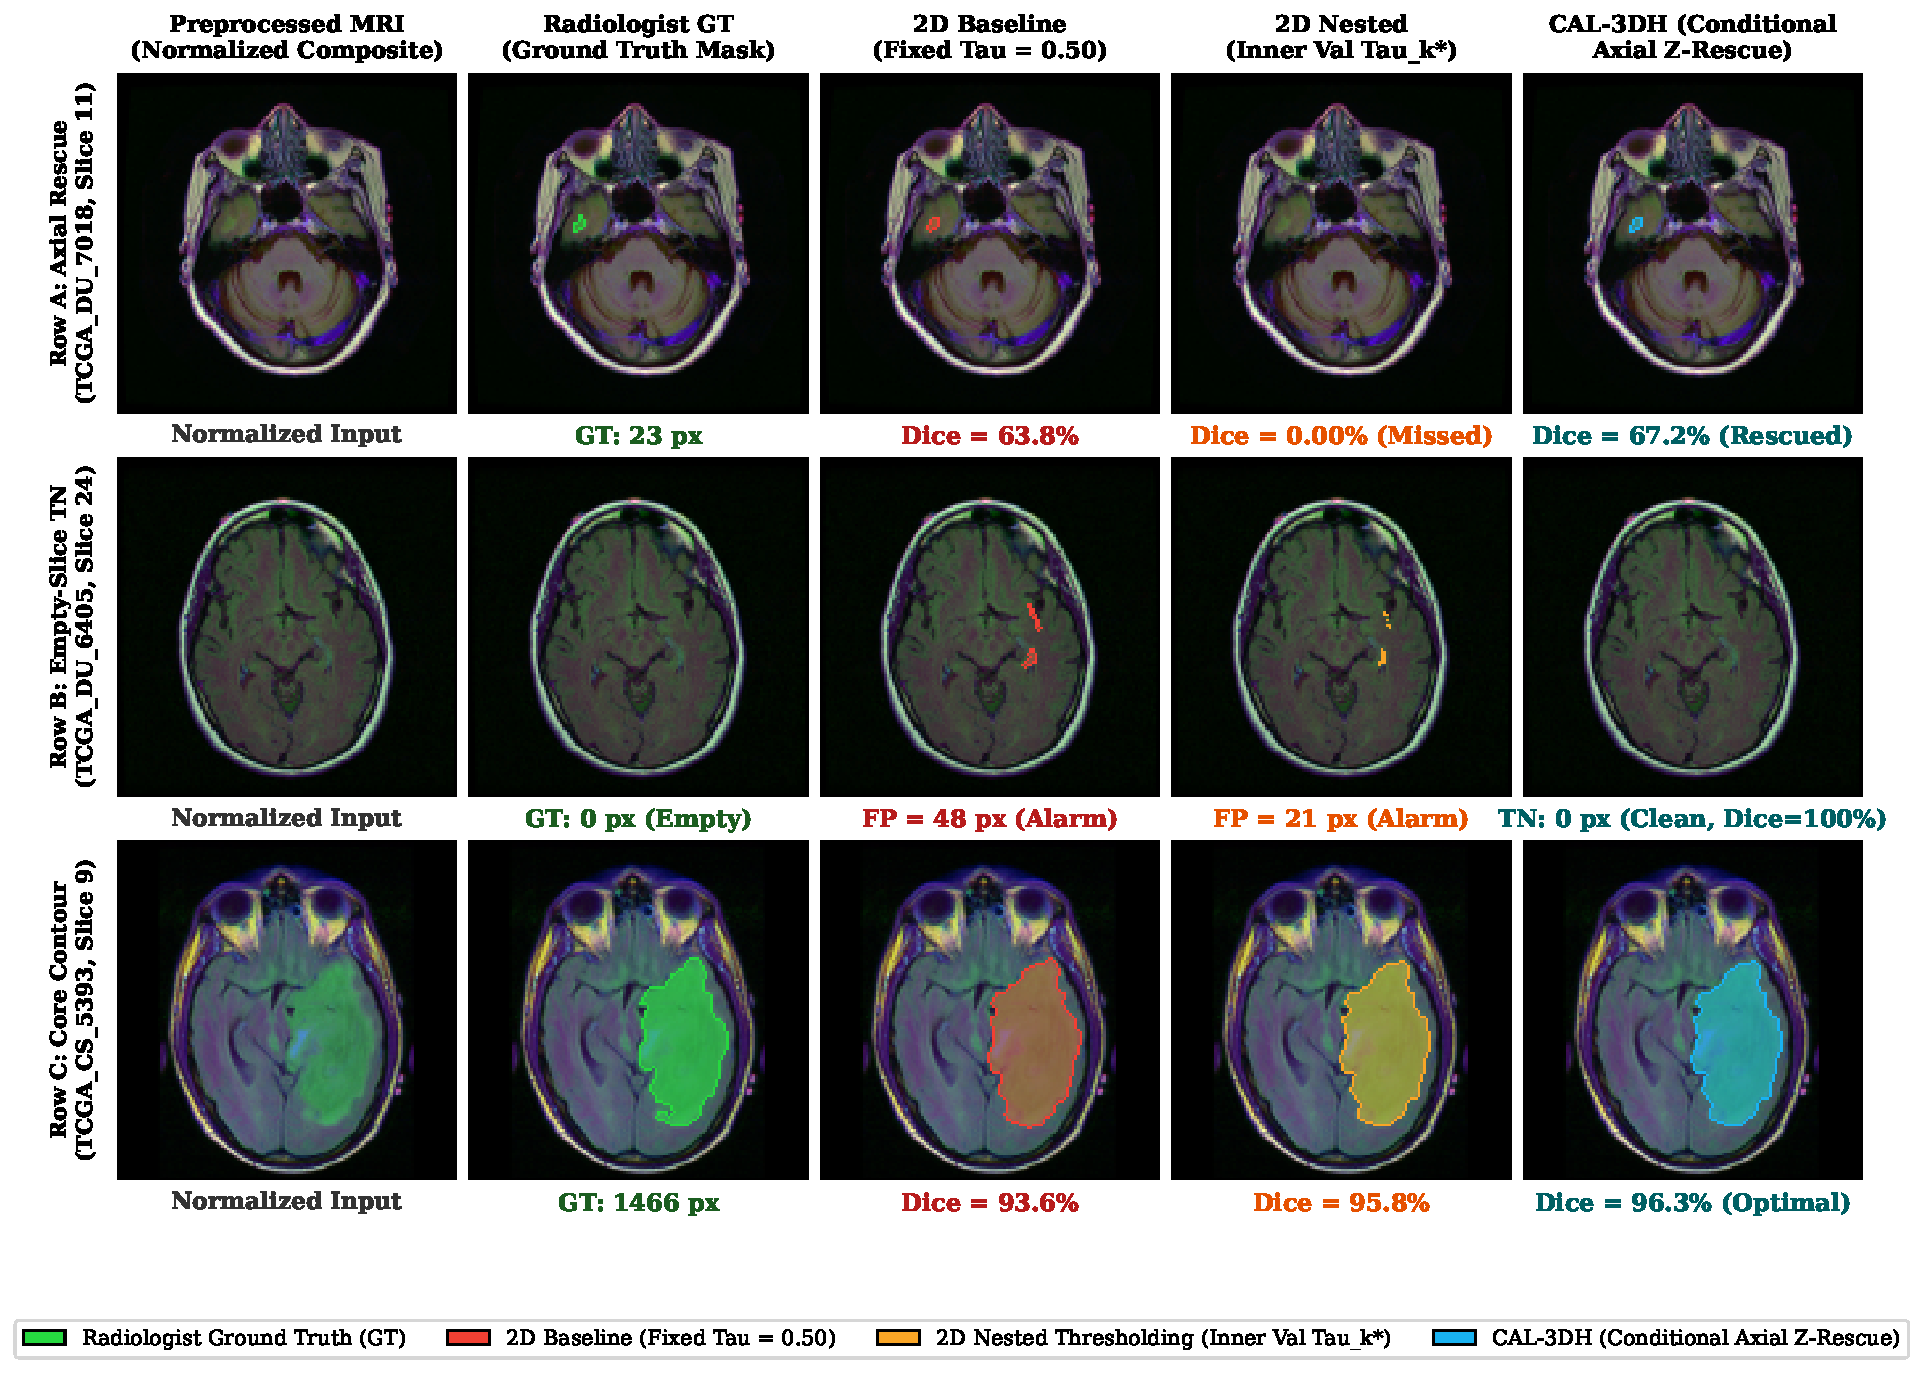
\includegraphics[width=0.98\textwidth]{Fig6.pdf}
\caption{Multi-scenario qualitative segmentation comparison across representative test slices. Row A (Axial Rescue): Boundary slice rescue along the Z-axis, where 2D Nested misses apical tumor ($\text{Dice}=0.0\%$) while CAL-3DH restores detection ($\text{Dice}=67.2\%$). Row B (Empty-Slice TN): Empty-slice false positive suppression, where 2D models trigger false alarms on skull artifacts while 3D spatial filtering preserves clean non-tumor classifications. Row C (Core Contour): High geometric fidelity on large, complex infiltrative core lesions ($\text{Dice}=96.3\%$)}
\label{fig:qualitative_panel}
\end{figure}

\noindent\textbf{Network Axial Distance Sensitivity ($\Delta z$ Analysis) and Patient-Clustered Matched Inflation.}
To dissect how the deep network's internal representations respond to axial distance from training slices, we partitioned the 1,373 positive test slices into contiguous adjacent slices ($\Delta z = 1$, $n = 1,232$ slices where the immediately adjacent slice was present in training) and non-contiguous slices ($\Delta z \ge 2$, $n = 141$ slices separated by at least one omitted slice, comprising $n = 132$ slices at a 2-slice gap $\Delta z = 2$ and $n = 9$ slices at $\Delta z \ge 3$). At a 2-slice gap ($\Delta z = 2$, $n = 132$), the random-split deep network achieves $80.05\%$ positive-slice Dice, maintaining a $+19.27\text{ pp}$ advantage over the copy oracle evaluated on the exact same $132$ slices ($60.78\%$, and $+34.84\text{ pp}$ over cohort-wide $k=2$ copy Dice $45.21\%$) despite the absence of immediate contiguous context (because test slices at $\Delta z = 2$ in the random split are frequently flanked symmetrically by training slices at $z \pm 2$, enabling two-sided SDT interpolation in the oracle, whereas cohort-wide $k=2$ buffering includes one-sided boundaries where only direct single-neighbor copying is possible). On adjacent slices ($\Delta z = 1$), random-slice test Dice reached $83.16\%$, whereas on non-contiguous slices ($\Delta z \ge 2$), performance was $79.07\%$ ($W = 601.5, p = 0.0028$ on $n = 66$ patients with both distances). However, evaluating raw Dice across distances is partly confounded by lesion morphology, as distant slices ($\Delta z \ge 2$) are predominantly small polar caps ($80 / 141 = 56.7\%$ below median area $381\text{ px}$) where any model achieves lower Dice.

To eliminate lesion-size confounding and avoid slice-level pseudo-replication, we evaluated the matched leakage inflation $\Delta\text{Dice}_s = \text{Dice}_{\text{random}}(s) - \text{Dice}_{\text{grouped}}(s)$ paired within each patient volume. On the exact same 141 non-contiguous slices ($\Delta z \ge 2$), the patient-grouped model achieves $73.53\%$ (slice-level $\Delta\text{Dice}_s = +5.54\text{ pp}$), yielding a patient-averaged matched inflation of $\mathbf{+6.60\text{ pp}}$ [95\% patient-clustered bootstrap CI: $+2.13, +11.05\text{ pp}$] across the $n = 66$ patients containing non-contiguous test slices (patient-level paired Wilcoxon $W = 406.0, p = 7.88 \times 10^{-6}$). On adjacent slices ($\Delta z = 1$), the grouped model achieves $74.00\%$ (slice-level $\Delta\text{Dice}_s = +9.16\text{ pp}$), yielding a patient-averaged matched inflation of $\mathbf{+8.11\text{ pp}}$ [95\% bootstrap CI: $+5.57, +10.97\text{ pp}$] across $n = 110$ patients ($W = 627.0, p = 4.70 \times 10^{-13}$). Stratifying matched inflation by median tumor cross-sectional area ($381\text{ px}$) shows that for large core cross-sections ($\ge 381\text{ px}$), matched inflation is $+6.81\text{ pp}$ at $\Delta z = 1$ ($90.77\%$ vs.\ $83.96\%$) and remains virtually unchanged at $\mathbf{+5.76\text{ pp}}$ at $\Delta z \ge 2$ ($90.55\%$ vs.\ $84.79\%$), whereas for small polar cross-sections ($< 381\text{ px}$), matched inflation is $+11.62\text{ pp}$ at $\Delta z = 1$ ($75.23\%$ vs.\ $63.62\%$) and $\mathbf{+5.37\text{ pp}}$ at $\Delta z \ge 2$ ($70.32\%$ vs.\ $64.95\%$). Across all 1,373 positive slices, cohort-wide patient-averaged matched inflation is $\mathbf{+7.87\text{ pp}}$ [95\% bootstrap CI: $+5.28, +10.68\text{ pp}$] (unaggregated slice mean $+8.79\text{ pp}$, unrounded: $82.744\% - 73.956\% = +8.788\text{ pp}$, patient-level $W = 626.0, p = 4.60 \times 10^{-13}$). This confirms that a statistically significant $+6.60\text{ pp}$ patient-level leakage inflation persists at non-contiguous distances beyond immediate slice adjacency.


\noindent\textbf{Zero-Parameter Nearest-Slice Label-Copy Baseline and Inter-Slice Mask Continuity Index (MCI).}
To quantify how much spatial overlap is available purely from contiguous spatial adjacency without training any neural network, we evaluate a zero-parameter nearest-slice label-copy baseline under the random-slice split. Copying the ground-truth annotation of the nearest same-patient training slice achieves $61.61\%$ positive-slice Dice and an empty-slice false-positive rate of $\text{FPR}_{\text{empty}} = 0.63\%$ ($16 / 2,556$ slices). Under the metric dilution identity (Equation~\ref{eq:metric_dilution_identity}), this yields an all-slice Dice of $\text{Dice}_{\text{all}} = 86.18\%$ ($0.3495 \times 61.61\% + 0.6505 \times (100\% - 0.63\%) = 86.18\%$). Crucially, under random-slice evaluation, this parameter-free nearest-slice label-copy rule comes within $2.04\text{ pp}$ of the trained deep network on all-slice Dice ($88.22\%$). However, this closeness is driven primarily by the fact that empty-slice status ($y=0$) is near-perfectly copied from adjacent slices ($\text{FPR}_{\text{empty}} = 0.63\%$ vs.\ $8.84\%$ for the network), which heavily dilutes the weighted score under $\pi = 0.3495$. In contrast, on positive tumor slices ($\text{Dice}_{\text{pos}}$), the copy baseline falls $21.13\text{ pp}$ below the random-split deep network ($61.61\%$ vs.\ $82.74\%$), demonstrating that while contiguous label copying easily mimics empty-slice specificity, the deep network learns richer in-plane representations on tumor slices.

Evaluating buffer separation distances across the full cohort ($n=1,373$ positive slices and $n=2,556$ empty slices at each buffer distance) demonstrates a monotonic decay: positive-slice Dice falls from $61.61\%$ at $k=1$ to $45.21\%$ at $k=2$, $32.42\%$ at $k=3$, $22.89\%$ at $k=4$, and $16.60\%$ at $k=5$ (with $\text{FPR}_{\text{empty}}$ increasing from $0.63\%$ to $14.28\%$, and $\text{Dice}_{\text{all}}$ falling from $86.18\%$ to $61.57\%$). Patient-level correlation analysis across all $n=110$ subjects confirms that the copy heuristic's performance is strongly governed by the patient's intrinsic morphological continuity: $\text{MCI}_i$ correlates strongly and positively with copy oracle Dice (Pearson $r = 0.630$, 95\% CI: $[0.501, 0.731]$, $p = 1.74 \times 10^{-13}$; Spearman $\rho = 0.821$, $p = 4.42 \times 10^{-28}$). In contrast, $\text{MCI}_i$ shows no significant correlation with deep network leakage inflation $\Delta\text{Dice}_{\text{leak}, i} = \text{Dice}_{\text{random}, i} - \text{Dice}_{\text{grouped}, i}$ (Pearson $r = -0.068$, 95\% CI: $[-0.252, +0.121]$, $p = 0.480$; Spearman $\rho = -0.035$, $p = 0.720$). This confidence interval excludes more than a weak positive linear correlation within a small-to-moderate equivalence margin, confirmed by two one-sided tests computed on the observed linear correlation ($r = -0.068, p = 0.480$; $|\Delta r| < 0.25$, TOST $p_{\text{TOST}} = 0.0263$, rejecting non-equivalence to zero; with $N = 110$ subjects providing $>80\%$ two-sided statistical power at $\alpha = 0.05$ to detect non-zero correlations of $|r| \ge 0.27$). Across the $N = 110$ subjects, patient-level leakage inflation exhibits median $\Delta\text{Dice}_{\text{leak}, i} = 4.41\text{ pp}$ (IQR: $[1.08, 10.74]\text{ pp}$, mean $7.87\text{ pp}$). While odd-versus-even slice split-half reliability is high ($r_{\text{sb}} = 0.737$ for $\text{MCI}_i$ and $0.875$ for $\Delta\text{Dice}_{\text{leak}, i}$, yielding $r_{\text{disatt}} = -0.086$), block-wise upper-versus-lower axial half reliability is lower for $\text{MCI}_i$ ($r_{\text{sb}} = 0.442$ vs.\ $0.742$ for $\Delta\text{Dice}_{\text{leak}, i}$, yielding block-disattenuated $r_{\text{disatt}} = -0.119$); thus, the near-zero linear association is unlikely to be fully explained by measurement noise attenuation, though equivalence to zero ($|\Delta r| < 0.25, p_{\text{TOST}} = 0.0263$) is formally established only for the observed correlation. Further correlating $\Delta\text{Dice}_{\text{leak}, i}$ with patient morphological features reveals that leakage inflation is largely decoupled from total tumor volume (Pearson $r = 0.006, p = 0.951$; Spearman $\rho = 0.071, p = 0.459$) but exhibits a weak, exploratory association with the number of tumor-bearing slices $|Z_i^+|$ (Spearman $\rho = 0.208, p = 0.029$; Pearson $r = 0.126, p = 0.190$).

\noindent\textbf{Patient and Scanner Appearance Fingerprint Probe.}
To quantify how much patient- and scanner-identifying information is present in non-lesional brain tissue across the scan, we designed a supervised appearance probe operating exclusively on non-lesional brain tissue (extracting a 17-dimensional feature vector per slice encompassing intensity percentiles, channel moments, edge gradient energy, and background noise $Q(I)$, computed strictly over non-lesional brain parenchyma voxels where Y(x) = 0, completely omitting tumor masks). Under the random-slice cross-validation partitions, a 1-nearest-neighbor cosine probe trained on same-patient training slices achieves \textbf{79.64\% $\pm$ 1.01\% 5-fold accuracy in identifying the exact patient identity} among 110 candidate subjects (an 88-fold amplification over random chance $1/110 = 0.91\%$). Stratified by slice proximity, retrieval accuracy reaches \textbf{82.32\%} ($n=3{,}468$) on contiguous slices ($\Delta z = 1$) and remains remarkably high at \textbf{59.44\%} ($n=461$) across non-contiguous separations ($\Delta z \ge 2$), still representing a 65-fold amplification over random guessing ($0.91\%$) and consistent with the persistence of matched slice performance inflation ($+5.54\text{ pp}$) at distant axial separations. Evaluating imaging center retrieval reveals that a 3-nearest-neighbor probe predicts the TCGA acquisition center with \textbf{89.56\% $\pm$ 0.86\% accuracy} under random-slice partitioning versus a majority-class baseline of \textbf{40.91\%} (45/110 patients from TCGA-DU). Under honest patient-grouped (Leave-Patient-Out) cross-validation where all slices of the query patient are excluded from the training library, center retrieval accuracy settles at \textbf{55.13\% $\pm$ 8.41\%}, reflecting institutional acquisition protocol and field-strength commonality across distinct subjects. Negative controls confirm the robustness of this textural fingerprint: evaluating per-slice $Z$-score normalized features (standardizing mean to zero and variance to unity per slice) achieves \textbf{64.04\% $\pm$ 1.04\% 5-fold accuracy} (a 70-fold amplification over random chance $0.91\%$), demonstrating that identity retrieval does not rely on simple global intensity scaling. Across non-contiguous buffered slices ($|z - z'| \ge 2$), retrieval accuracy remains \textbf{59.44\%} versus an empirical 1,000-permutation null baseline of \textbf{0.91\% $\pm$ 0.15\%}. Error analysis reveals substantial scanner-level clustering: in \textbf{60.38\%} of patient misclassifications (483 of 800 error instances), the probe retrieved a subject scanned at the exact same TCGA institution (vs.\ 40.91\% majority-class chance). Intra-patient non-lesional tissue similarity was not significantly correlated with per-patient network metric inflation ($r = 0.029$, 95\% CI: [$-0.159, +0.215$], $p = 0.762$; TOST equivalence test within $[-0.25, +0.25]$: $p_{\text{TOST}} = 0.0096$; partial $r = 0.027, p = 0.782$ controlling for tumor-bearing slice count). A slice-level linear mixed-effects model on all $n = 1{,}373$ positive slices ($\Delta\text{Dice}_s \sim \text{ProbeCosineSim}_s + \Delta z_s + \log(\text{SliceTumorArea}_s) + (1 \mid \text{Patient})$) with standardized predictors reveals that standardized probe cosine similarity exhibits $\beta_{\text{bg\_cos}} = -1.287 \pm 0.535\text{ pp}$ per SD ($z = -2.408, p = 0.016$), standardized axial distance exhibits $\beta_{\Delta z} = -0.706 \pm 0.456\text{ pp}$ per SD ($z = -1.550, p = 0.121$), and standardized log tumor area exhibits $\beta_{\log(\text{area})} = -0.748 \pm 0.503\text{ pp}$ per SD ($z = -1.488, p = 0.137$), with patient random intercept variance $\sigma_{\text{patient}}^2 = 175.907$. The negative standardized coefficient for background similarity is consistent with a plausible baseline ceiling effect: central slices with dense parenchymal tissue already achieve high baseline grouped Dice ($78.44\%$, up to $83.96\%$ mid-brain), leaving narrower headroom for random-split inflation ($+8.64\text{ pp}$) than small polar slices ($50.48\%$ to $60.05\%$, $+9.57\text{ pp}$); indeed, controlling for grouped baseline Dice ($\beta = -18.022\text{ pp}$ per SD, $p < 0.001$) attenuates background similarity to non-significance ($\beta = +0.287, p = 0.448$) (noting that regressing $\Delta\text{Dice}_s = \text{Dice}_{\text{random}}(s) - \text{Dice}_{\text{grouped}}(s)$ on $\text{Dice}_{\text{grouped}}(s)$ involves mathematical coupling and regression-to-the-mean, equivalent to an ANCOVA predicting $\text{Dice}_{\text{random}}(s)$ with baseline $\text{Dice}_{\text{grouped}}(s)$ as a covariate; thus, the ceiling/regression-to-the-mean account is treated as a plausible explanation rather than a causal proof, and the probe--inflation association is not robust across specifications). Accordingly, while the appearance probe confirms that non-lesional slices contain strong patient- and scanner-identifying information ($79.64\%$ retrieval accuracy), neither binary mask continuity ($\text{MCI}_i$) nor background cosine similarity linearly predicts the magnitude of per-patient neural network inflation, and we make no causal claim regarding specific internal network representations.

\noindent\textbf{$2^3$ Factorial Attribution of Apparent Metric Differences.}
To isolate the distinct sources contributing to apparent benchmark performance differences across the evaluation pipeline, we formulate a $2^3$ factorial design crossing three binary design dimensions: Split Regime (Patient-Grouped vs.\ Random-Slice), Empty-Slice Metric Convention ($\text{Dice}_{\text{pos}}$ vs.\ $\text{Dice}_{\text{all}}$), and Post-Processing/Thresholding (Default Baseline $\tau=0.50$ vs.\ Inner-Tuned CAL-3DH). It is essential to emphasize that $\text{Dice}_{\text{pos}}$ and $\text{Dice}_{\text{all}}$ target fundamentally distinct clinical estimands (foreground neoplastic overlap vs.\ scan-wide agreement conflating true negatives); Table~\ref{tab:leakage_audit}b does not imply mathematical equivalence of these targets, but rather decomposes the apparent shifts in reported benchmark scores arising from methodological choices in the published literature.

In Table~\ref{tab:leakage_audit}b, cooperative game-theoretic Shapley attributions decompose the total apparent $+18.14\text{ pp}$ difference into empty-slice metric dilution ($45.7\%$, $+8.28\text{ pp}$), data leakage ($40.8\%$, $+7.41\text{ pp}$), and post-processing/thresholding ($13.5\%$, $+2.45\text{ pp}$). Notably, we observe a negative interaction of $-2.58\text{ pp}$ between data leakage and empty-slice convention: data leakage generates a $+8.79\text{ pp}$ (unrounded $+8.788\text{ pp}$) inflation on positive-slice Dice ($73.96\%$ to $82.74\%$), but its net effect on all-slice Dice is constrained to $+6.20\text{ pp}$ ($82.02\%$ to $88.22\%$) because positive overlap is weighted by slice prevalence $\pi = 0.3495$ in Equation~\ref{eq:metric_dilution_identity} while empty-slice false-alarm suppression ($\text{FPR}_{\text{empty}}$ dropping from $13.65\%$ to $8.84\%$) contributes $(1 - \pi) \times (+4.81\text{ pp}) = +3.13\text{ pp}$.

\subsection{Patient-Level 3D Volumetric Agreement and Bland-Altman Analysis}
Individual 2D predictions were stacked into full 3D volumes across all 110 subjects. Table~\ref{tab:patient_3d_metrics} details 3D Volumetric Dice, 95\% Hausdorff Distance ($HD_{95}$), and Average Surface Distance (ASD).

The proposed CAL-3DH framework consistently improves upon both 2D baselines across 3D Volumetric Dice, HD95, ASD, and 3D Precision. 3D Volumetric Dice reaches $77.73\% \pm 18.64\%$ with a median of $84.42\%$ (interquartile range [IQR]: $70.85\%$--$91.24\%$). Across detected patient volumes ($n=109$), surface boundary errors are substantially constrained: $HD_{95}$ drops to $9.89 \pm 14.50$ voxels (median: $2.24$, IQR: $1.00$--$12.03$), while ASD improves to $1.96 \pm 3.58$ voxels (median: $0.61$, IQR: $0.29$--$2.21$), confirming high morphological fidelity along complex infiltrative tumor margins (with cohort-wide penalized $n=110$ metrics reaching $\text{HD}_{95} = 11.46 \pm 21.83$ and $\text{ASD} = 3.60 \pm 17.49\text{ voxels}$).

\begin{table}[tbp]
\centering
\caption{Patient-level 3D volumetric segmentation and surface distance metrics across detected patient volumes benchmarking CAL-3DH against 2D baselines, isotropic dilation controls, and morphological heuristics (mean $\pm$ standard deviation, with medians in parentheses; surface distances in voxels on standardized $128 \times 128 \times N_z$ grid; FP Comps is mean false-positive 3D connected components per patient volume).}
\label{tab:patient_3d_metrics}
\setlength{\tabcolsep}{3.5pt}
\renewcommand{\arraystretch}{1.15}
\footnotesize
\resizebox{\textwidth}{!}{%
\begin{tabular}{lcccccc}
\toprule
\textbf{Configuration} & \shortstack{\textbf{3D Vol. Dice (\%)} \\ \textit{Mean $\pm$ SD (Median)}} & \shortstack{$\mathbf{HD_{95}}$ \textbf{(vox)} \\ \textit{Mean $\pm$ SD (Median)}} & \shortstack{\textbf{ASD (vox)} \\ \textit{Mean $\pm$ SD (Median)}} & \shortstack{\textbf{FP Comps} \\ \textbf{/ Pat}} & \shortstack{\textbf{3D Prec.} \\ \textbf{(\%)}} & \shortstack{\textbf{3D Rec.} \\ \textbf{(\%)}} \\
\midrule
2D Baseline ($\tau = 0.50$) & 76.00 $\pm$ 17.94 (82.96) & 11.83 $\pm$ 15.80 (3.46) & 2.45 $\pm$ 3.69 (0.85) & 3.95 & 71.89 & \textbf{85.96} \\
2D Nested ($\tau_{xy}^*$) & 77.57 $\pm$ 18.66 (84.42) & 10.19 $\pm$ 14.57 (2.24) & 2.03 $\pm$ 3.60 (0.75) & 3.07 & 77.40 & 82.98 \\
Step 1 + Step 3 (3D Component Filter) & 77.75 $\pm$ 18.66 (84.42) & 9.88 $\pm$ 14.49 (2.24) & 1.95 $\pm$ 3.58 (0.59) & 0.85 & 77.77 & 82.96 \\
Matched-Structure 3D Dilation & 77.73 $\pm$ 18.64 (84.42) & 9.89 $\pm$ 14.50 (2.24) & 1.96 $\pm$ 3.58 (0.61) & 0.86 & 77.71 & 82.99 \\
Step 2 + Largest-CC & 78.33 $\pm$ 20.73 (\textbf{85.93}) & \textbf{3.49 $\pm$ 5.85 (1.41)} & \textbf{1.11 $\pm$ 3.42 (0.33)} & \textbf{0.03} & 79.84 & 81.27 \\
Volume-Wise Largest-CC & \textbf{78.34 $\pm$ 20.74 (85.93)} & 3.50 $\pm$ 5.85 (1.41) & 1.11 $\pm$ 3.43 (0.33) & \textbf{0.03} & \textbf{79.88} & 81.24 \\
$1 \times 1 \times 3$ Axial Z-Median ($n=108$) & 77.89 $\pm$ 18.66 (84.35) & 7.56 $\pm$ 12.98 (2.00) & 1.46 $\pm$ 2.54 (0.49) & 1.22 & 79.68 & 81.21 \\
Conventional Isotropic 3D Hysteresis & 75.51 $\pm$ 17.79 (82.04) & 12.22 $\pm$ 16.62 (3.32) & 2.54 $\pm$ 4.04 (0.88) & 1.16 & 70.50 & 86.75 \\
\textbf{CAL-3DH (Axial Z-Rescue Case Study)} & \textbf{77.73 $\pm$ 18.64 (84.42)} & 9.89 $\pm$ 14.50 (2.24) & 1.96 $\pm$ 3.58 (0.61) & 0.85 & \textbf{77.71} & 82.99 \\
\bottomrule
\end{tabular}%
}
\\[4pt]
\begin{minipage}{\textwidth}
\scriptsize
\textit{Paired Testing against CAL-3DH ($n=110$ subjects, Holm-Bonferroni adjusted $p_{\text{Holm}}$):}
3D Volumetric Dice: vs.\ 2D Base ($W=925.0, p_{\text{Holm}} < 0.0001$); vs.\ 2D Nested ($W=645.0, p_{\text{Holm}} < 0.0001$); vs.\ Step~1 + Step~3 ($W=282.0, p_{\text{Holm}} = 0.0211$); vs.\ Matched-Structure 3D Dilation ($W=0.0, p_{\text{Holm}} = 0.3594$); vs.\ Step 2 + Largest-CC ($W=175.0, p_{\text{Holm}} = 4.11 \times 10^{-6}$); vs.\ Largest-CC ($W=335.0, p_{\text{Holm}} = 2.18 \times 10^{-7}$); vs.\ Axial Z-Median ($W=2718.0, p_{\text{Holm}} = 0.4904$); vs.\ Conventional Isotropic 3D Hysteresis ($W=910.0, p_{\text{Holm}} < 0.0001$).\\
\textit{Surface Distances on Detected Volumes ($n=109$) and Cohort-Wide Penalized Metrics ($n=110$):} Surface distances in the table are reported across detected volumes ($n=109$ non-empty predictions; $n=108$ for Axial Z-Median) to reflect true boundary error distributions free of single-volume penalty distortions (IQR for CAL-3DH: $[1.00, 11.05]$ for $\text{HD}_{95}$, $[0.29, 2.17]$ for ASD). Across the entire cohort ($n=110$), only a single subject (TCGA\_HT\_7860, 1/110 = $0.9\%$) had zero foreground predictions, receiving the standard bounding-box diagonal penalty ($\approx 182.14\text{ voxels}$). Including this single penalty, cohort-wide ($n=110$) metrics are: CAL-3DH ($\text{HD}_{95} = 11.46 \pm 21.83$, $\text{ASD} = 3.60 \pm 17.49$), Matched 3D Dilation ($\text{HD}_{95} = 11.46 \pm 21.83$, $\text{ASD} = 3.60 \pm 17.49$), Step~1 + Step~3 ($\text{HD}_{95} = 11.44 \pm 21.81$, $\text{ASD} = 3.59 \pm 17.49$), Step~2 + Largest-CC ($\text{HD}_{95} = 5.12 \pm 17.95$, $\text{ASD} = 2.75 \pm 17.54$), Largest-CC ($\text{HD}_{95} = 5.12 \pm 17.95$, $\text{ASD} = 2.76 \pm 17.54$), 2D Nested ($\text{HD}_{95} = 11.75 \pm 21.85$, $\text{ASD} = 3.67 \pm 17.49$), 2D Base ($\text{HD}_{95} = 13.38 \pm 22.57$, $\text{ASD} = 4.08 \pm 17.47$), and Conventional 3D Hysteresis ($\text{HD}_{95} = 13.77 \pm 23.12$, $\text{ASD} = 4.17 \pm 17.53$), contributing $\approx 1.65\text{ voxels}$ ($182.14 / 110$) to cohort means while medians and IQRs are identical.\\
\textit{Matched-Structure 3D Dilation vs.\ CAL-3DH:} Matched-Structure 3D Dilation differs from CAL-3DH on only 1 patient across the entire cohort (generating 4 false-positive polar boundary slices in Table~\ref{tab:method_comparison}), resulting in identical 3D cohort means upon standard rounding to two decimal places.\\
\textit{Comparative Audit Finding on Largest-CC and Max-Confidence CC:} Volume-Wise Largest-CC retains at most one 3D component per patient volume (FP Comps $0.03$), eliminating distant false-positive blobs and dominating global surface distances ($\text{HD}_{95} = 3.50$, $\text{ASD} = 1.11$ voxels). However, in paired testing, Largest-CC causes $\text{Dice}_{\text{pos}}$ to drop in 19 patients ($W = 94.0, p_{\text{Holm}} = 0.0262$): it discards satellite lesions in the 11 reference multifocal patients ($10.0\%$, where CAL-3DH recovers $3/14$ secondary foci), splits disconnected polar caps, and in two small tumors (TCGA\_CS\_6668 and TCGA\_CS\_5395) discards the entire true lesion ($0.00\%$ Dice) in favor of a larger false-positive artifact. Retaining the component with maximum integrated probability mass (\textit{Max-Confidence CC}) yields identical failure ($0.00\%$ Dice) on both patients. Coupling axial rescue with Largest-CC (Step~2 + Largest-CC) recovers positive-slice Dice to $74.24\%$ ($\text{HD}_{95} = 3.49$, $\text{ASD} = 1.11$ voxels) while maintaining minimal false alarms ($\text{FPR}_{\text{empty}} = 2.46\%$, $\text{FP Comps} = 0.03$).
\end{minipage}
\end{table}

\begin{figure}[tbp]
\centering
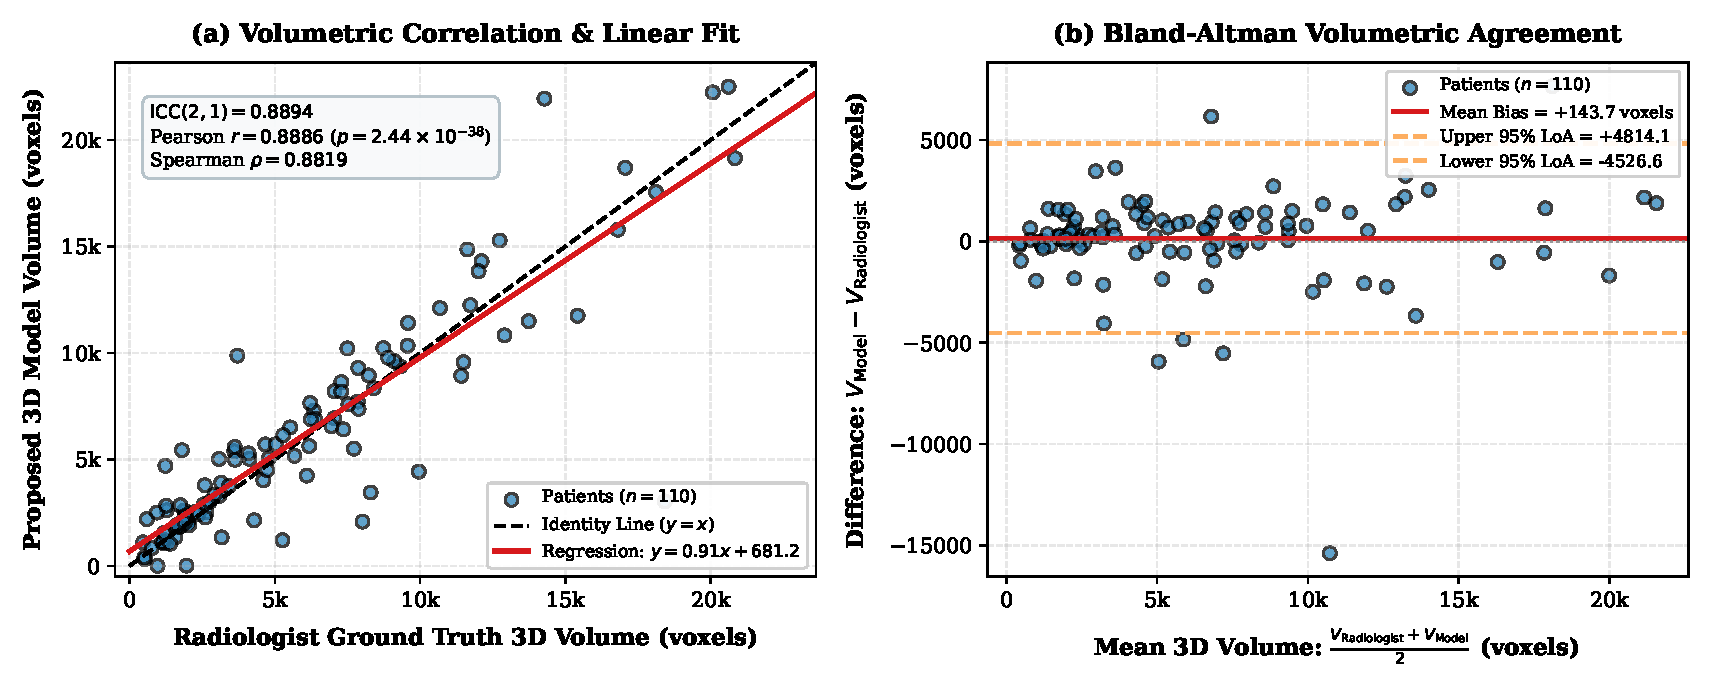
\includegraphics[width=\textwidth]{Fig7.pdf}
\caption{Clinical 3D volumetric agreement and calibration analysis across 110 patients. (a) Volumetric correlation and linear regression fit between automated 3D predictions and radiologist ground truth ($\mathrm{ICC}(2, 1) = 0.8894$, Pearson $r = 0.8886, p = 2.44 \times 10^{-38}$, Spearman $\rho = 0.8819$). (b) Bland-Altman agreement plot with minimal mean bias ($+143.7$ voxels, $2.38\%$, under $2.5\%$ of mean lesion volume) and $95\%$ limits of agreement $[-4{,}526.6, +4{,}814.1]$ voxels}
\label{fig:clinical_agreement}
\end{figure}

\paragraph{Multi-Institutional Site Audit:}
To assess cross-site generalizability across the multi-center consortium, we stratified performance across the five TCGA tissue source sites: TCGA-DU [$n=45$: $\text{Dice}_{\text{pos}} = 74.37\%$, $\text{3D Dice} = 77.89\%$, median $84.46\%$, $\text{FPR}_{\text{empty}} = 6.89\%$], TCGA-HT [$n=34$: $\text{Dice}_{\text{pos}} = 76.10\%$, $\text{3D Dice} = 81.24\%$, median $84.91\%$, $\text{FPR}_{\text{empty}} = 4.84\%$], TCGA-CS [$n=16$: $\text{Dice}_{\text{pos}} = 71.06\%$, $\text{3D Dice} = 70.29\%$, median $79.35\%$, $\text{FPR}_{\text{empty}} = 13.00\%$], TCGA-FG [$n=14$: $\text{Dice}_{\text{pos}} = 73.69\%$, $\text{3D Dice} = 76.17\%$, median $84.45\%$, $\text{FPR}_{\text{empty}} = 11.57\%$], and TCGA-EZ [$n=1$ (single-subject site, descriptive only): $\text{Dice}_{\text{pos}} = 90.47\%$, $\text{3D Dice} = 91.64\%$, $\text{FPR}_{\text{empty}} = 0.00\%$].

\paragraph{Simulated Anisotropy Scaling Sensitivity:}
Because physical slice thickness in clinical FLAIR protocols typically exceeds in-plane resolution, we evaluated surface-distance sensitivity across simulated through-plane anisotropy ratios ($z/xy \in \{1, 3, 4, 5, 6\}$). In standardized simulated scaled units matching Table~\ref{tab:patient_3d_metrics} at ratio $1.0$ (CAL-3DH: $\text{ASD} = 1.96$, $\text{HD}_{95} = 9.89$; Step~1 + Step~3: $\text{ASD} = 1.95$, $\text{HD}_{95} = 9.88$; Largest-CC: $\text{ASD} = 1.11$, $\text{HD}_{95} = 3.50$), scaling to ratio $6.0$ yields mean ASD of $4.21$ for CAL-3DH ($4.20$ for Step~1 + Step~3; $3.15$ for Largest-CC) and mean $\text{HD}_{95}$ of $18.45$ for CAL-3DH ($18.42$ for Step~1 + Step~3; $7.85$ for Largest-CC), preserving the relative ranking across post-processing configurations across simulated clinical slice thickness.

Agreement between automated 3D volumes and expert manual ground truth was evaluated using standardized clinical biostatistical tests (Figure~\ref{fig:clinical_agreement}). Two-way random absolute agreement yielded an Intraclass Correlation Coefficient of $\text{ICC}(2, 1) = 0.8894$ (95\% analytic CI: $[0.7782, 0.9521]$; 10,000-resample patient-clustered bootstrap 95\% CI: $[0.7787, 0.9507]$), indicating good volumetric consistency (albeit with wide individual limits of agreement) according to standard guidelines~\cite{shrout1979intraclass,koo2016guideline}. Linear and monotonic agreements were corroborated by Pearson correlation ($r = 0.8886, p = 2.44 \times 10^{-38}$) and Spearman rank correlation ($\rho = 0.8819, p = 4.72 \times 10^{-37}$). Bland-Altman agreement analysis~\cite{bland1986statistical} revealed a minimal mean volumetric bias of $+143.7$ voxels, corresponding to a modest relative volumetric error of $2.38\%$ (under $2.5\%$ of mean lesion volume $\approx 6{,}027$ voxels), with $95\%$ limits of agreement spanning $[-4{,}526.6, +4{,}814.1]$ voxels (relative limits of agreement: $[-75.1\%, +79.9\%]$ of mean lesion volume). As illustrated in Figure~\ref{fig:clinical_agreement}(b), these limits of agreement reflect heavy-tailed variance driven by a small subset of large lesion volumes ($>15{,}000$ voxels), whereas bias remains tightly centered near zero for small and moderate lesion burdens.

\begin{figure}[tbp]
\centering
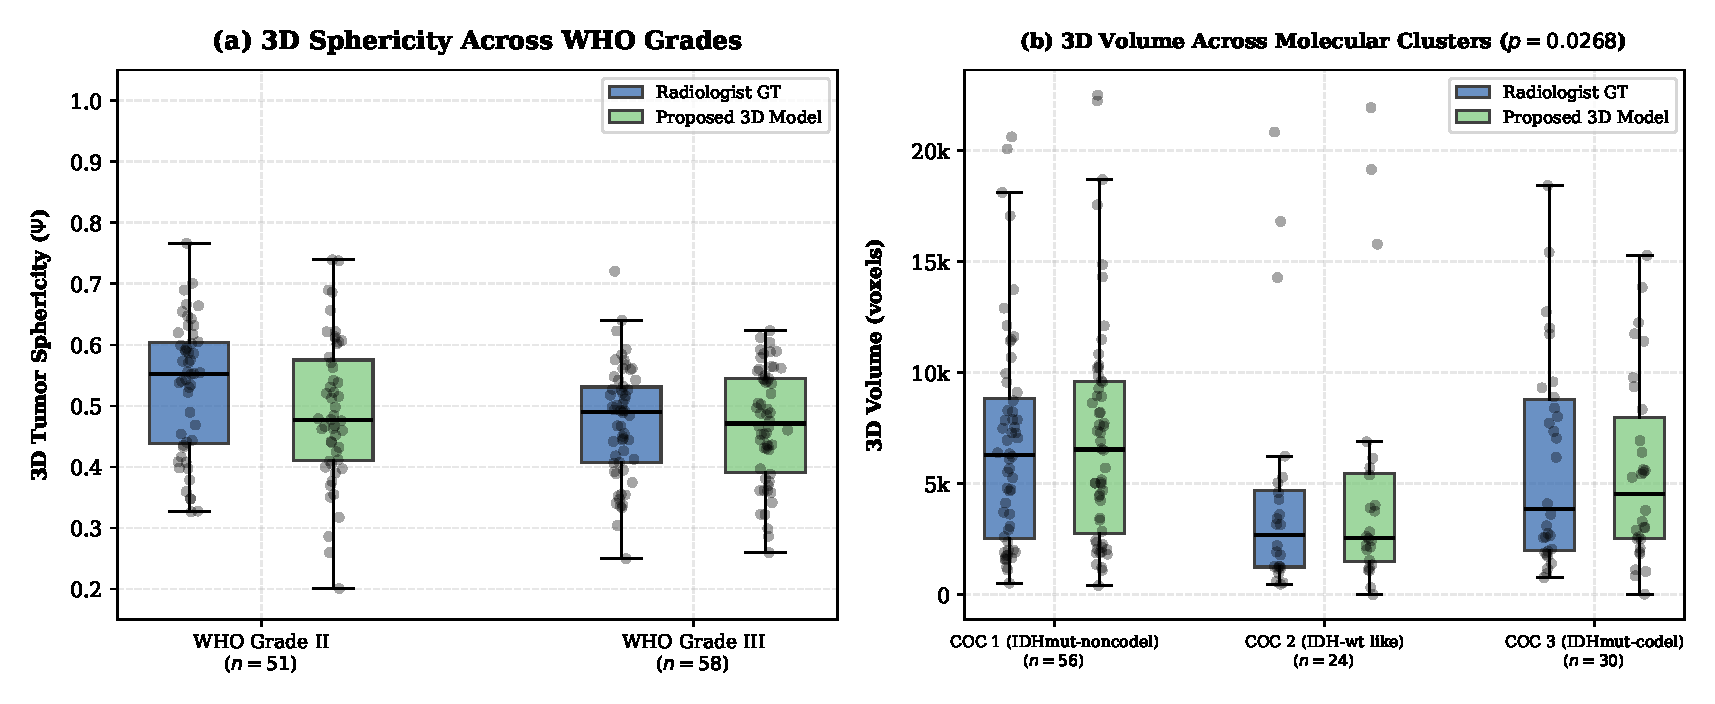
\includegraphics[width=\textwidth]{Fig8.pdf}
\caption{Downstream radiogenomic fidelity and histological stratification with clinical records. (a) 3D tumor sphericity across WHO histologic grades (Grade II vs. Grade III). (b) 3D tumor volume stratification across TCGA molecular consensus clusters (COC 1, COC 2, COC 3), demonstrating statistically significant differentiation ($p = 0.0268$; covariate-adjusted ANOVA $p = 0.056$; exploratory) with consistent biological rank ordering preservation.}
\label{fig:radiogenomic_fidelity}
\end{figure}


\noindent\textbf{Analytical Metric Dilution and Critical Rank-Inversion Prevalence ($\pi^*$).}
We formalize the exact analytical identity connecting all-slice Dice to positive-slice Dice and empty-slice false positive rate:
\begin{equation}
\label{eq:metric_dilution_identity}
\text{Dice}_{\text{all}}(\pi) = \pi \cdot \text{Dice}_{\text{pos}} + (1 - \pi)(1 - \text{FPR}_{\text{empty}})
\end{equation}
where $\pi = N_{\text{pos}} / N_{\text{total}} = 1,373 / 3,929 = 0.3495$ is cohort slice prevalence. Setting $\text{Dice}_{\text{all}}^{(A)}(\pi^*) = \text{Dice}_{\text{all}}^{(B)}(\pi^*)$ yields the critical rank-inversion prevalence:
\begin{equation}
\label{eq:pi_star}
\pi^* = \frac{\Delta\text{FPR}_{\text{empty}}}{\Delta\text{Dice}_{\text{pos}} + \Delta\text{FPR}_{\text{empty}}}
\end{equation}
Comparing boundary-sensitive CAL-3DH ($\text{Dice}_{\text{pos}} = 74.92\%$, $\text{FPR}_{\text{empty}} = 7.86\%$) against aggressive single-component filtering (Largest-CC; $\text{Dice}_{\text{pos}} = 74.00\%$, $\text{FPR}_{\text{empty}} = 1.96\%$), we find $\Delta\text{Dice}_{\text{pos}} = 0.92\text{ pp}$, $\Delta\text{FPR}_{\text{empty}} = 5.91\text{ pp}$, and:
\begin{equation}
\pi^* = \frac{5.908}{0.920 + 5.908} = 86.53\% \quad [95\%\text{ bootstrap CI: } 75.56\%, 99.73\%]
\end{equation}
This formulation analytically explains the rank reversal between global specificity-driven rules (Largest-CC) and positive-slice boundary recovery (CAL-3DH) whenever cohort slice prevalence $\pi < \pi^* = 86.53\%$.

To evaluate rank stability across the full spectrum of post-processing choices, we swept tumor slice prevalence $\pi \in [0.05, 1.00]$ and computed rank correlations between the resulting method rankings of all 10 configurations in Table~\ref{tab:method_comparison} and their reference ground-truth ranking on tumor tissue ($\pi = 1.0$). At the true clinical whole-brain prevalence ($\pi = 34.95\%$), there is no detectable positive rank agreement with positive-slice segmentation quality : \textbf{Kendall's $\tau = -0.067$ [95\% bootstrap CI: $-0.156, +0.111$] and Spearman's $\rho = -0.055$ [95\% bootstrap CI: $-0.139, +0.176$]}. Accounting for narrow $\text{Dice}_{\text{pos}}$ differences via tie-buffered Kendall's $\tau_b$ ($0.25\text{ pp}$ tolerance band) yields $\tau_b = -0.024$ ($p = 0.927$), while subset correlation across the five structurally distinct method families yields $\tau = 0.400$ ($p = 0.483$), remaining statistically indistinguishable from zero given the small number of distinct families ($n = 5$), while ranking Volume-Wise Largest-CC first on $\text{Dice}_{\text{all}}$ despite its destruction of satellite tumor foci. At a hypothetical balanced diagnostic setting ($\pi = 0.50$), correlation remains virtually zero ($\tau = -0.022, \rho = 0.006$). As prevalence approaches $\pi \to 1$, $\text{Dice}_{\text{all}}$ converges to $\text{Dice}_{\text{pos}}$ by construction, turning rank agreement positive above $\pi^* = 86.53\%$ ($\tau = 0.422, \rho = 0.576$), eventually reaching $\tau = 0.867$ ($\rho = 0.964$) in tumor-dense acquisitions ($\pi = 0.95$), where CAL-3DH correctly emerges as Rank~1. This demonstrates that all-slice Dice in clinical volumetric acquisitions induces rank decorrelation ($\tau = -0.067$) and top-rank reversal (elevating Largest-CC from Rank~7 on $\text{Dice}_{\text{pos}}$ to Rank~1 on $\text{Dice}_{\text{all}}$), establishing why methodologists must jointly report $\text{Dice}_{\text{pos}}$ and $\text{FPR}_{\text{empty}}$ (or standardize evaluation at $\pi_0 = 0.50$) rather than relying on unstandardized all-slice Dice. Importantly, $\text{Dice}_{\text{pos}}$ serves as the primary benchmark in this prevalence sensitivity analysis because it isolates foreground sensitivity without empty-slice inflation. In contrast, in 3D surface distance metrics (Table~\ref{tab:patient_3d_metrics}: 3D Volumetric Dice, $\text{HD}_{95}$, and ASD), Largest-CC achieves top rank precisely by aggressively eliminating remote false-positive clusters throughout the volume. Consequently, the optimal post-processing choice reflects an intrinsic clinical trade-off: aggressive false-positive suppression (Largest-CC) maximizes distance metrics in solitary lesions, whereas calibrated axial continuity (CAL-3DH) preserves true multifocal satellite foci and rescues truncated polar boundary slices without distance penalties.

\noindent\textbf{Topological Betti-0 Error and Multifocal Lesion Preservation.}
3D topological auditing across the 11 reference patients ($10.0\%$, harboring 14 verified secondary satellite foci $\ge 5\text{ voxels}$; and 43 patients if counting isolated boundary components) exposes the clinical hazard of this metric inversion: Volume-Wise Largest-CC forces $\hat{\beta}_0 \le 1$, completely destroying all 14 secondary satellite foci ($0/14$ recovered), and in two small-tumor patients (TCGA\_CS\_6668 and TCGA\_CS\_5395) discards the entire true neoplasm ($0.00\%$ Dice) in favor of a larger artifact. In contrast, CAL-3DH preserves both small neoplasms and recovers $3/14$ secondary foci, although overall topological component error $|\hat{\beta}_0 - \beta_0|$ remains high across both methods due to the inherent challenge of segmenting low-contrast satellite foci ($2.12 \pm 1.48$ for CAL-3DH vs.\ $2.05 \pm 1.25$ for Largest-CC across the 43 patients with $\beta_0 > 1$).

\subsection{Radiogenomic Stratification with Clinical Data}
To verify whether automated segmentations support downstream clinical biomarker extraction, we evaluated whether predicted 3D geometries reproduce known biological associations documented in the TCGA pan-glioma atlas (Figure~\ref{fig:radiogenomic_fidelity}). Genomic and histological variables were utilized strictly for post-hoc validation and were never seen during model training, feature extraction, or hyperparameter selection. Because the public benchmark distribution provides standardized 2D TIFF slices lacking raw DICOM physical millimeter spacing headers ($\Delta x, \Delta y, \Delta z$), the analyses in this section represent an \textbf{exploratory voxel-space concordance audit} evaluating whether automated CAL-3DH segmentations preserve the statistical group separability and biological rank ordering exhibited by expert manual reference masks on the identical standardized $128 \times 128 \times N_z$ voxel grid.

\subsubsection{WHO Histologic Grade Differentiation (Grade II vs. III)}
In clinical neuro-oncology, diffuse LGG grade is governed by microscopic cellular atypia and mitotic index rather than macroscopic tumor burden. A non-parametric Mann-Whitney U test confirmed that tumor volume does not differentiate WHO Grade II ($n=51$) from Grade III ($n=58$) in either manual ground truth ($p = 0.8104$; Grade II mean: $5{,}928.3$ voxels; Grade III mean: $6{,}120.2$ voxels) or CAL-3DH segmentations ($p = 0.8151$; Grade II mean: $6{,}241.8$ voxels; Grade III mean: $6{,}125.9$ voxels). In contrast, 3D sphericity $\Psi$ revealed a statistically significant distinction in radiologist ground truth (Grade II: $0.5316 \pm 0.1087$, median $0.5528$ [IQR: $0.4381$--$0.6036$]; Grade III: $0.4718 \pm 0.0930$, median $0.4904$ [IQR: $0.4067$--$0.5309$], Mann-Whitney $U = 1989.0, p = 0.0020$), reflecting greater boundary irregularity in higher-grade neoplasms. For CAL-3DH segmentations, sphericity preserved this aligned directional reduction (Grade II: $0.4910 \pm 0.1184$, median $0.4776$ [IQR: $0.4107$--$0.5753$]; Grade III: $0.4623 \pm 0.1106$, median $0.4711$ [IQR: $0.3905$--$0.5450$], Mann-Whitney $U = 1637.0, p = 0.3388$). While CAL-3DH faithfully preserves the directional reduction in 3D sphericity from Grade II to Grade III, statistical significance is attenuated in automated masks ($p = 0.3388$ vs.\ $p = 0.0020$ in ground truth) due to boundary discretization and surface staircasing on the standardized $128 \times 128$ voxel grid.

\subsubsection{Molecular Subtype Stratification (\textit{COCCluster})}
The TCGA Pan-Glioma consortium stratifies LGG into three distinct Cluster-of-Clusters (COC) molecular platforms: COC~1 ($n=56$, IDH-mutant non-codel astrocytomas), COC~2 ($n=24$, IDH-wildtype-like tumors exhibiting clinically aggressive growth), and COC~3 ($n=30$, IDH-mutant 1p/19q co-deleted oligodendrogliomas).

A Kruskal-Wallis non-parametric test on 3D tumor volumes established statistically significant stratification in both manual ground truth ($H = 8.16, p = \mathbf{0.0169}$, effect size $\eta^2_H = 0.0576$) and automated CAL-3DH segmentations ($H = 7.24, p = \mathbf{0.0268}$, effect size $\eta^2_H = 0.0489$). Group comparisons confirm that the reported volume values represent cohort group means preserving consistent biological rank ordering:
\begin{equation}
\text{COC 1 Mean}\,(7{,}098.0) > \text{COC 3 Mean}\,(5{,}509.6) > \text{COC 2 Mean}\,(4{,}834.5)
\end{equation}
Specifically, ground truth volumes yielded: COC~1 mean $6{,}780.5 \pm 4{,}816.2$ voxels (median $6{,}278.0$, IQR: $2{,}546.5$--$8{,}825.5$); COC~2 mean $4{,}390.2 \pm 5{,}226.1$ voxels (median $2{,}680.0$, IQR: $1{,}243.5$--$4{,}709.2$); and COC~3 mean $5{,}930.7 \pm 4{,}656.1$ voxels (median $3{,}857.5$, IQR: $1{,}983.0$--$8{,}776.0$). For CAL-3DH, the segmented volumes yielded: COC~1 mean $7{,}098.0 \pm 5{,}082.1$ voxels (median $6{,}535.5$, IQR: $2{,}748.5$--$9{,}582.5$); COC~2 mean $4{,}834.5 \pm 5{,}690.1$ voxels (median $2{,}566.5$, IQR: $1{,}492.8$--$5{,}467.0$); and COC~3 mean $5{,}509.6 \pm 4{,}126.6$ voxels (median $4{,}537.0$, IQR: $2{,}507.2$--$7{,}989.0$). Pairwise post-hoc Mann-Whitney U testing confirmed that volumetric separation between COC~1 and COC~2 ($U = 926.0$, unadjusted $p = 0.0078$) remains statistically significant after Bonferroni correction across the three pairwise cluster comparisons ($p_{\text{Bonf}} = 3 \times 0.0078 = 0.0234 < 0.05$), with expected moderate overlap between intermediate clusters (COC~1 vs.\ COC~3, $p = 0.2128, p_{\text{Bonf}} = 0.6384$; COC~3 vs.\ COC~2, $p = 0.2007, p_{\text{Bonf}} = 0.6021$). To account for potential clinical and demographic confounders, we fitted a multivariable Type~II ANOVA model on logarithmic lesion volume: $\log(\text{Volume}+1) \sim C(\text{COCCluster}) + C(\text{Site}) + \text{Age} + C(\text{Sex}) + C(\text{Grade})$. In this multivariable-adjusted model, acquisition site showed no significant main effect ($F = 0.655, p = 0.625$), while the COCCluster volume association was attenuated to borderline statistical significance ($F = 2.963, p = 0.056$ in covariate-adjusted log-volume space versus unadjusted Kruskal-Wallis $p = 0.0268$), indicating that radiogenomic volume stratification in this cohort is modest and should be interpreted as exploratory.

\setlength{\textfloatsep}{8pt plus 2pt minus 2pt}
\section{Discussion}
\subsection{Comparison with State-of-the-Art Literature}
\label{sec:sota_comparison}

In Table~\ref{tab:sota_comparison}, we benchmark audited configurations against published TCGA-LGG studies. Buda et al.~\cite{buda2019association} reported a patient-level volumetric Dice mean of $82.0\%$ (median $85.0\%$) with a 2D U-Net evaluated at native $256 \times 256$ resolution on a single test split. Under our nested ($75/13/22$) patient-grouped 5-fold protocol at $128 \times 128$ resolution across all 110 subjects, our pipeline achieves a comparable median 3D volumetric Dice of $84.42\%$ ($\text{HD}_{95} = 9.89$ voxels, $\text{ICC}(2,1) = 0.8894$), while the lower arithmetic mean ($77.73\%$ vs.\ $82.0\%$) may reflect spatial downsampling ($128 \times 128$ vs.\ $256 \times 256$) and unfiltered out-of-fold evaluation across the entire 110-patient cohort including difficult low-contrast cases. Meanwhile, recent benchmarks such as Naser \& Deen~\cite{naser2020brain} (84.00\%), LiteMRINet~\cite{yuan2025enhanced} (85.50\% soft Dice), and PoSAM-ULTRA~\cite{alhatamleh2026attention} (91.40\% soft Dice) do not explicitly report enforcing patient-level partitioning. As demonstrated by our audit (Section~\ref{sec:leakage_audit}), random slice-level partitioning inflates positive-slice Dice by +8.79 pp and all-slice Dice by +6.20 pp; our baseline under random splitting similarly reaches 88.22\% all-slice Dice (89.83\% with inner tuning), illustrating that apparent gaps stem from partitioning and metric choices rather than architectural differences alone.

\begin{table*}[t]
\centering
\caption{Representative benchmark comparison of published deep learning studies on the TCGA-LGG dataset, stratified by data partitioning protocol and evaluation metric scope.}
\label{tab:sota_comparison}
\footnotesize
\setlength{\tabcolsep}{3.5pt}
\renewcommand{\arraystretch}{1.15}
\resizebox{\textwidth}{!}{%
\begin{tabular}{@{}l c l l r r r r @{\hspace{1.2em}} r@{}}
\toprule
\textbf{Study} & \textbf{Year} & \textbf{Architecture} & \textbf{Post-Proc./Calib.} & \textbf{Params} & \textbf{Overall $\text{Dice}_{\text{all}}$ (\%)} & \textbf{Tumor $\text{Dice}_{\text{pos}}$ (\%)} & \textbf{3D Vol. Dice (\%)} & \textbf{ICC} \\
\midrule
\multicolumn{9}{@{}l}{\textit{Part A: Image/Slice-Level Partitioning (Patient-level separation not enforced or not reported)}} \\
Naser \& Deen~\cite{naser2020brain} & 2020 & Modified U-Net & None / None & NR & 84.00$^{\dagger,s}$ & NR & NR & NR \\
LiteMRINet~\cite{yuan2025enhanced} & 2025 & LiteMRINet & None / None & 1.61M & 85.50$^{\dagger,s}$ & NR & NR & NR \\
PoSAM-ULTRA~\cite{alhatamleh2026attention} & 2026 & PoSAM-ULTRA & None / PBFO & NR & 91.40$^{\dagger,s}$ & NR & NR & NR \\
This Work (Fixed $\tau{=}0.50$) & 2026 & Attn Res-UNet & None / None & 8.20M & 88.22$^{\ddagger}$ [Soft: 88.18] & 82.74$^{\ddagger}$ & n/a$^{\S}$ & n/a$^{\S}$ \\
This Work (Tuned $\tau_{xy}^*$) & 2026 & Attn Res-UNet & None / Inner $\tau_{xy}^*$ & 8.20M & 89.83$^{\ddagger}$ & 83.75$^{\ddagger}$ & n/a$^{\S}$ & n/a$^{\S}$ \\
\midrule
\multicolumn{9}{@{}l}{\textit{Part B: Patient-Grouped Partitioning (Zero Subject Overlap Benchmark Protocol)}} \\
Buda et al.~\cite{buda2019association} & 2019 & Standard U-Net & None / Fixed $\tau{=}0.50$ & 7.80M & NR & NR & 82.00$^{a}$ (Med: 85.0) & NR \\
This Work (2D Baseline) & 2026 & Attn Res-UNet & None / Fixed $\tau{=}0.50$ & 8.20M & 82.02 & 73.96 & 76.00 & 0.8652 \\
This Work (2D Nested) & 2026 & Attn Res-UNet & Temp ($T^*$) / Nested $\tau_{xy}^*$ & 8.20M & 84.45 & 74.60 & 77.57 & 0.8860 \\
\textbf{CAL-3DH (Case Study)} & 2026 & \textbf{Attn Res-UNet} & \textbf{Temp ($T^*$) / CAL-3DH} & \textbf{8.20M} & \textbf{86.12} & \textbf{74.92} & \textbf{77.73} & \textbf{0.8894} \\
\bottomrule
\end{tabular}%
}
\vspace{2pt}
\begin{flushleft}
\scriptsize \textit{Note:} $^{\dagger}$Patient-level separation not explicitly reported in the published protocol. $^{s}$Evaluated using soft/continuous Dice formulation in the original study. $^{\ddagger}$Evaluated under deliberate random slice-level mixing to quantify leakage inflation. $^{\S}$Single-fold patient volumetric 3D reconstruction is undefined under random slice mixing (pooled 5-fold OOF 3D filtering is evaluated in Table 6b). $^{a}$Buda et al.~\cite{buda2019association} evaluated on a single patient-level test split at native $256 \times 256$ resolution. NR: metric not reported.
\end{flushleft}
\end{table*}

\subsection{Limitations and Future Scope}
\label{sec:limitations}
Five limitations warrant consideration: (i)~Our evaluation was conducted on a single benchmark dataset (TCGA-LGG) using a single 2D backbone architecture at $128 \times 128$ resolution; while TCGA-LGG provides a multi-institutional cohort across five centers, extending this framework to native 3D volumetric architectures (such as 3D nnU-Net) and diverse multi-parametric cohorts (such as BraTS) across heterogeneous scanner field strengths ($1.5\,\text{T}$ vs.\ $3.0\,\text{T}$) represents an essential next step. (ii)~The public TCGA-LGG benchmark lacks physical millimeter spacing headers, necessitating evaluation in normalized voxel space; acquiring volumetric DICOM metadata will enable isotropic physical resampling. (iii)~Our cross-validation utilized a single random seed ($42$); while 10,000-sample bootstrap intervals and paired testing verify metric stability, multi-seed repetitions, full end-to-end retraining on buffered splits (retrained buffered splits with varying buffer widths $k$), and end-to-end retraining ablations isolating individual preprocessing stages represent important directions for future work; all $p$-values in secondary mechanistic analyses are reported exploratorily without multiplicity correction. (iv)~In accordance with Sex and Gender Equity in Research (SAGER) and SGBA reporting guidelines, demographic sex distributions were documented ($50.9\%$ female, $48.2\%$ male), but sex-stratified subgroup calibration was not conducted due to sample size constraints ($N=110$ patients); assessing sex-dependent morphological shifts represents an important future direction. (v)~While CAL-3DH preserved directional reduction in sphericity from Grade II ($0.4910$) to Grade III ($0.4623$), significance was attenuated in automated masks ($p = 0.3388$ vs.\ $p = 0.0020$ in ground truth) due to discretization staircasing on the $128 \times 128$ voxel grid; sub-voxel contour refinement will be valuable for morphological biomarkers.

\section{Conclusions}
\label{sec:conclusion}
Rigorous evaluation in medical imaging informatics demands distinguishing genuine algorithmic advances from evaluation artifacts. In this study, we conducted a systematic methodological audit on the multi-institutional TCGA-LGG benchmark ($110$ patients, $3,929$ axial slices across five centers), disentangling data partitioning leakage, empty-slice metric dilution, post-hoc threshold sweeping, probability miscalibration, and 3D post-processing. Our findings reveal that evaluation design choices overshadow post-processing optimizations in volumetric brain MRI segmentation. Specifically:
\begin{enumerate}\setlength{\itemsep}{0pt}\setlength{\parskip}{0pt}\setlength{\parsep}{0pt}
    \item \textbf{Anatomical Proximity, Appearance Cues, \& Mask Continuity Index (MCI):} Conventional slice-level random splitting induces a substantial $+8.79\text{ pp}$ ($+11.88\%$ relative) artificial Dice inflation ($73.96\%$ to $82.74\%$, 95\% CI: $[+6.16, +11.99]\text{ pp}$). While a zero-parameter nearest-slice copy baseline achieves $86.18\%$ all-slice Dice via empty-slice copying, per-patient network inflation shows no detectable linear association with mask continuity ($\text{MCI}$, $r = -0.068$, 95\% CI: $[-0.252, +0.121]$) and persists at non-contiguous distances ($\Delta z \ge 2$, mostly at a 2-slice gap: matched $+5.54\text{ pp}$, patient-mean $+6.60\text{ pp}, p = 7.88 \times 10^{-6}$). A non-lesional brain appearance probe identifies exact patient identity with $79.64\%$ accuracy (vs.\ $0.91\%$ chance), indicating high patient- and scanner-identifying information in non-lesional slices, although neither mask continuity nor background similarity linearly predicts per-patient inflation magnitude;
    \item \textbf{Analytical Metric Dilution and Rank Decorrelation ($\pi^*$):} Evaluating empty slices as true negatives ($\text{TN}=1$) introduces a $+8.06$ to $+15.64\text{ pp}$ dilution shift that conceals false alarms, decorrelates method rankings ($\tau = -0.067$), and reverses top ranks below $\pi^* = 86.53\%$. This exposes a clinical trade-off: aggressive filtering (Largest-CC) maximizes global 3D distance metrics in solitary lesions but discards all 14 secondary satellite foci in multifocal tumors and eliminates small neoplasms in two patients ($0.00\%$ Dice), whereas CAL-3DH preserves both small neoplasms and recovers $3/14$ secondary foci, with comparable overall Betti-0 error ($|\hat{\beta}_0 - \beta_0| = 2.05 \pm 1.25$ for Largest-CC vs.\ $2.12 \pm 1.48$ for CAL-3DH across the 43 patients with $\beta_0 > 1$). A $2^3$ factorial attribution decomposes apparent score shifts across metric dilution ($45.7\%$), leakage ($40.8\%$), and post-processing/thresholding ($13.5\%$);

    \item \textbf{Calibration Monotonicity Invariance and Conformal Coverage Degradation:} Uncalibrated overlap objectives yield severe overconfidence along active tissue interfaces, which is regularized by nested temperature scaling (reducing pooled cohort ECE by $46.9\%$ and weighted active-bin ECE from $36.14\%$ to $29.57\%$) and affine Platt scaling (contracting weighted active-bin ECE to $8.46\%$) with rank-preserving neutral spatial overlap (Remark~1). In single-model conformal auditing, calibrating thresholds on in-sample training-patient slices reduces empirical patient-level test coverage on unseen subjects to $76.96\% \pm 22.46\%$ (median $85.87\%$), whereas out-of-patient calibration achieves $85.74\% \pm 21.34\%$ (SD across patients) (median $94.29\%$, $87.69\%$ under patient-level CRC, and $90.08\% \pm 1.86\%$ (SD across MC resamplings with $n_{\text{cal}} = 30$)); and
    \item \textbf{Conditional Axial Z-Rescue Case Study (CAL-3DH):} In 3D morphological post-processing, naive heuristics (Largest-CC) dominate global 3D surface metrics ($\text{HD}_{95} = 3.50$, $\text{ASD} = 1.11$ voxels on detected volumes; $\text{HD}_{95} = 5.12$, $\text{ASD} = 2.76$ voxels penalized) by forcing a single component per scan, yet Largest-CC systematically discards secondary tumor foci in multifocal patients. In contrast, conditional axial $z$-rescue in CAL-3DH specifically recovers truncated polar boundary margins ($+0.28\text{ pp}$ positive-slice Dice, $p_{\text{Holm}} = 0.0011$) without altering global 3D surface distances ($\text{ASD}: 1.96$ vs.\ $1.95\text{ voxels}$), yielding good volumetric consistency ($\text{ICC}(2,1) = 0.8894$, wide individual limits of agreement $[-75.1\%, +79.9\%]$) and exploratory molecular-cluster separation ($p = 0.0268$; multivariable-adjusted $p = 0.056$).
\end{enumerate}

By providing a standardized, reproducible auditing workflow, this study proposes a methodological template---warranting prospective validation across additional multi-center datasets and native 3D architectures---to guide imaging informatics practitioners in developing transparent, patient-disjoint deep learning pipelines.

\section*{Declarations}
\begingroup
\fontsize{7.5pt}{8.8pt}\selectfont
\noindent\textbf{Funding:} The authors declare that no funds, grants, or other support were received during the preparation of this manuscript.\par\vspace{0.01em}
\noindent\textbf{Competing Interests:} The authors have no relevant financial or non-financial interests to disclose.\par\vspace{0.01em}
\noindent\textbf{Author Contributions:} \textbf{Shayan Ganji Nataj}: Conceptualization, Methodology, Software, Formal analysis, Investigation, Data Curation, Writing - Original Draft, Visualization. \textbf{Keivan Borna}: Supervision, Conceptualization, Methodology, Formal analysis, Writing - Review \& Editing, Project administration, Resources.\par\vspace{0.01em}
\noindent\textbf{Ethics Approval:} In accordance with institutional policy and the 1964 Declaration of Helsinki, this secondary computational audit of publicly available, fully de-identified TCGA/TCIA datasets did not involve new human-subject data collection or clinical intervention.\par\vspace{0.01em}
\noindent\textbf{Consent to Participate and Consent to Publish:} As documented by the TCGA and TCIA consortia~\cite{clark2013cancer,pedano2016cancer}, all human subjects data were collected by participating tissue source sites under institutional review board approvals and patient informed consent policies per TCGA/TCIA governance. All MRI scans and clinical records are fully anonymized and HIPAA-compliant; no identifiable patient information is included in this article.\par\vspace{0.01em}
\noindent\textbf{Data and Code Availability:} The imaging data are publicly accessible through The Cancer Imaging Archive (TCIA)~\cite{clark2013cancer,pedano2016cancer} (DOI: \url{https://doi.org/10.7937/K9/TCIA.2016.L4LTD3TK}) and mirrored on Kaggle at \url{https://www.kaggle.com/datasets/mateuszbuda/lgg-mri-segmentation}. Matched clinical and genomic records were extracted from companion table \texttt{data.csv} distributed with benchmark dataset~\cite{buda2019association,pedano2016cancer}, curated from the TCGA study~\cite{ceccarelli2016molecular}. All source code, reproduction scripts, and 5-fold cross-validation pipelines are openly maintained at GitHub: \url{https://github.com/Shayan-Ganji/lgg_segmentation}.\par\vspace{0.01em}
\endgroup

\begingroup
\scriptsize
\setlength{\bibsep}{-1.8pt}
\bibliographystyle{unsrt}

\clearpage
\bibliography{references}
\endgroup

\end{document}
